\documentclass[a4paper, titlepage, 12pt]{article}

% ------------------------------------------------------------
% LATEX SETUP
% ------------------------------------------------------------
% padding
\usepackage[left=3cm, right=3cm, top=3cm, bottom=3cm]{geometry}

% input packages
\usepackage[utf8]{inputenc}
\usepackage[T1]{fontenc}
\usepackage{blindtext}
\usepackage{nameref} % cross-referencing sections by name

% layout of ToC & appendix
\usepackage[toc,titletoc,title]{appendix}

% better tables
\usepackage{booktabs}
\usepackage{multirow}

\usepackage{printlen}

% math stuff
\usepackage{amsmath}
\usepackage{amssymb}
\usepackage{derivative}

% hyphenation, highlighting, URLs, spacing
\usepackage{setspace}
\usepackage{soul}
\usepackage{enumitem}
\usepackage{array}
\usepackage{makecell}
\usepackage[hidelinks]{hyperref}
\usepackage{adjustbox}
\usepackage{csquotes}

% Graphics and TikZ stuff
\usepackage{color}
\usepackage{graphicx}
\usepackage{tikz}
\usetikzlibrary{arrows}
\usetikzlibrary{arrows.meta,positioning}

% better captioning
\usepackage{caption}
\usepackage{subcaption}
% \usetikzlibrary{calc}

% TikZ settings
\usetikzlibrary{intersections}
\tikzset{>=latex}
\tikzstyle{curve}=[very thick,line cap=round]
\pgfdeclarelayer{back} % to draw on background
\pgfsetlayers{back,main} % set order
\usepackage{ifthen}
\usetikzlibrary{shapes.geometric}

% set up captions the way I like
\captionsetup[figure]{font=small, labelfont=bf, labelsep=period}
\captionsetup[table]{font=small, labelfont=bf, labelsep=period}
% \newcommand{\bcaption}[2]{\caption{\textbf{#1} #2}}
\newcommand{\bcaption}[2]{\caption[#1]{\textbf{#1} #2}}

% define custom SIR colours
\definecolor{s-color}{HTML}{41949A}
\definecolor{i-color}{HTML}{E56E5A}
\definecolor{r-color}{HTML}{7384BB}

% prefer roman numeral subfigures
\renewcommand\thesubfigure{\roman{subfigure}}

% TODO notes stuff
\setlength {\marginparwidth}{2cm}
\usepackage[textwidth=2.5cm]{todonotes} % add argument 'disable' to disable

% redefine the \todo command to always have small text and 0.5 spacing
\makeatletter
\renewcommand{\todo}[2][]{%
    \@todo[size=small, caption={#2}, #1]{\begin{spacing}{0.5}#2\end{spacing}}%
} 
\makeatother 

% enable highlighting of specific words with notes
\makeatletter
 \if@todonotes@disabled
 \newcommand{\hlnote}[2]{#1}
 \else
 \newcommand{\hlnote}[2]{\todo{#2}\texthl{#1}}
 \fi
\makeatother

% stop texcount from counting the words in todonotes.
%TC:macro \todo 1
%TC:macro \hlnote 2

% configure references
\usepackage[bibstyle=ieee, citestyle=numeric-comp, url=false]{biblatex}
\newcommand{\citet}{\textcite}
\addbibresource{refs.bib}
\renewcommand*{\bibfont}{\small}

% use microtype for better formatting (apparently)
\AtBeginEnvironment{quote}{\par\singlespacing\small}
\usepackage{microtype}

% create macro for quotations
\newcommand{\q}[1]{``#1''}

% create macro for ODD protocol
\newcommand{\odd}[1]{
\vspace{.5cm}
\textit{#1}
\vspace{.5cm}
}

% present objectives nicely
\newlist{objectives}{enumerate}{2}
\setlist[objectives,1]{label=\textbf{Objective \arabic*.},ref=\arabic*}
\setlist[objectives,2]{label=(\alph*),ref=\thequestionsi(\alph*)}

% use 1.5 line spacing as outlined in rubric
\onehalfspacing


% ------------------------------------------------------------
% DOCUMENT SETUP
% ------------------------------------------------------------
% title
\newcommand{\thesisTitle}{Simulating the Effects of Human Behaviour on Vector-borne Disease Spread with Agent-based Modelling}

% name
\newcommand{\name}{Jack Oliver}

% school
\newcommand{\timeFrame}{School of Computing and Information Systems}
\newcommand{\school}{The University of Melbourne}

% supervisors
\newcommand{\supervisor}{Associate Professor Nic Geard}
\newcommand{\advisor}{Dr Cameron Zachreson}

% ------------------------------------------------------------
% TITLE PAGE
% ------------------------------------------------------------
\begin{document}

%TC:ignore
\begin{singlespace} % single spacing for the cover page
\begin{titlepage}
\begin{center}
\vspace*{1.5cm}

\Large{\textbf{\thesisTitle}}
\vspace{2.5cm}

\large{by \name { }(1389498)} \\
\vspace{2cm}

\large{A final report submitted for the Master of Computer Science minor thesis component \\}
\vspace{.5cm}

\large{in the} \\
\large{\timeFrame} \\ 
\large{\textbf{\school}}
\vspace{2cm}

\large{\textbf{Primary Supervisor}}\\
\supervisor\\
\vspace{1.5cm}

\textbf{Co-Supervisor}\\
\advisor\\
\end{center}
\end{titlepage}
\end{singlespace}

% ------------------------------------------------------------
% FRONT MATTER
% ------------------------------------------------------------
\pagenumbering{roman}

\section*{Abstract}
\addcontentsline{toc}{section}{Abstract}

Vector-borne diseases (VBDs) such as malaria and dengue represent approximately 17\% of all infectious diseases globally. While traditional mathematical models are useful for predicting disease spread, these models often neglect individual risk perceptions and behavioural attitudes that influence preventive measure use, and consequently, infection dynamics. Computational techniques such as agent-based models (ABMs) have emerged to more accurately capture heterogeneous factors of VBD spread, yet most ABMs still employ simple representations of behaviour, despite a wealth of psychological literature on how individuals change their behaviour in disease contexts. 

Although prior work has implemented conceptual behaviour change theories (BCTs) into ABMs, the methodological implications of their integration into VBD models remain unclear, and no studies have compared the effects of implementing different BCTs. This thesis addresses this research gap by investigating how incorporating different BCTs within ABMs of VBD spread can influence the dynamics of preventive behaviours and disease spread.

In this work, I extend an ABM of VBD spread with preventive measures, and I parameterise the model to a real-world setting. Drawing on existing mathematical formulations, I implement two psychological BCTs and simulate hypothetical scenarios to assess their impacts on preventive behaviours, infection dynamics, and the model's alignment to real-world observations. I show that integrating BCTs into ABMs can lead to nuanced representations of behaviour that enable mechanistic explanations for preventive measure use, and I demonstrate how this could be useful for designing health interventions. However, I also show that different BCTs can yield distinct results within the same model, and that their computational implementations can be highly sensitive to small variations in their inputs and formulations.

Overall, this thesis illustrates the methodological implications of integrating different BCTs into models of disease spread, and contributes a foundational model of VBD spread that captures complex patterns of preventive behaviours which can inform future work.

% Vector-borne diseases (VBDs) such as malaria and dengue remain global health concerns, representing approximately 17\% of all infectious diseases. Mathematical models have emerged as useful tools to anticipate and understand the spread of such diseases, guiding policy and responses to disease outbreaks. However, these models have historically neglected important heterogeneous factors of risk perception and behavioural attitudes that influence the preventive behaviours of at-risk individuals. To address this, computational techniques such as agent-based models (ABMs) have been used to incorporate heterogenous factors of disease spread.

% Although ABMs have become widely adopted in the field of VBD modelling, most models use simple representations of human behaviour, despite a wealth of literature from psychology describing how individuals change their behaviour when at risk of disease. While prior work has integrated behaviour change theories into ABMs, the methodological implications of integrating such theories into models in VBD contexts is not clear, and little attention has been paid to the effects of using two different behaviour change theories. Evidently, there exists a gap in understanding around how computationally implementations of conceptual behaviour change theories within ABMs of VBD spread can influence the dynamics of preventive behaviours, and consequently, disease spread.

% To address this, I extend a general ABM of VBD spread with preventive measures, I parameterise the model to a real-world setting, and I implement two psychological behaviour change theories. I simulate hypothetical scenarios to assess the model's alignment to real-world observations, in addition to how incorporating behaviour change theories influences preventive behaviours and infection dynamics. I show that integrating behaviour change theories into ABMs can lead to nuanced representations of behaviour that enable mechanistic explanations for preventive measure use within at-risk populations. I demonstrate how this could be useful for designing health interventions. However, I also show that different behaviour change theories can lead to different results in the same base model, and that the computational implementations of such theories can be highly sensitive to small changes in behavioural dynamics.

% Overall, this thesis demonstrates the methodological implications of integrating behaviour change theories into models of disease spread, and . This thesis lays the groundwork of a general framework for modelling VBD spread with integrated behaviour change theories and preventive measures that can be extended in future work.

\clearpage

\section*{Declaration}
\addcontentsline{toc}{section}{Declaration}

I, Jack Oliver, on the 27th of October 2024, certify that:
\begin{itemize}
    \item this thesis does not incorporate, without acknowledgement, any material previously submitted for a degree or diploma in any university; and that to the best of my knowledge and belief it does not contain any material previously published or written by another person where due reference is not made in the text.
    \item no clearance from the University's Ethics Committee was necessary to carry out this research.
    \item the thesis is 22,923 words in length (excluding text in images, table, bibliographies and appendices).
\end{itemize}

\clearpage

\section*{Acknowledgements}
\addcontentsline{toc}{section}{Acknowledgements}

I extend my sincere gratitude to my supervisors Associate Professor Nic Geard and Dr Cameron Zachreson for their incredibly valuable and well-informed advice, surprising responsiveness to emails, witty and tasteful humour, persistent encouragement, and willingness to defend (and critique) my work. I thank them for somehow finding time each week to discuss my project while managing a multitude of other commitments. \\

\noindent I am incredibly fortunate to have been financially supported entirely throughout this degree by the Airwallex Excellence in Technology Masters Scholarship and the University of Melbourne Graduate Scholarship. I am also in a place of privilege to be supported by my parents, both personally and financially. \\

\noindent I am greatly indebted to my friends, coworkers, and loved ones for their continuous guidance, support, advice, and extended patience with me as I attempted to juggle full-time work and school.

\clearpage

\begin{spacing}{1.25} % custom-spaced ToC; adjust as necessary
    \tableofcontents
\end{spacing}
\clearpage

{
\footnotesize
\listoftables
}
\clearpage

{
\footnotesize
\listoffigures
}
\clearpage


% ------------------------------------------------------------
% MAIN MATTER
% ------------------------------------------------------------
\pagenumbering{arabic}
%TC:endignore

\section{Introduction}\label{sec:introduction}

%Vector-borne diseases (VBDs) such as malaria, dengue, and chikungunya are major public health concerns, representing approximately 17\% of all infectious diseases and causing over 700,000 deaths annually \cite{world_health_organisation_who_vector-borne_2020}.  While vector control methods such as mosquito repellents and insecticide-treated bed nets effectively reduce disease transmission, these methods rely primarily on self-participation and voluntary adoption, which are driven by individuals' perceived risk of infection and personal behavioural attitudes. Mathematical models have become increasingly popular to help health practitioners anticipate downward pressure on health infrastructure and guide policy decisions for outbreak responses \cite{reiner_systematic_2013}. However, these models assume homogeneity of populations and thus cannot incorporate heterogeneous human behavioural attitudes that influence participation in vector control. Individual- or agent-based modelling is a computational technique that simulates the individual components (\textit{agents}) of a system to generate complex phenomena indirectly \cite{epstein_growing_1996}, offering a solution for directly encoding human behaviour. Despite the existing success of agent-based models in VBD applications, however, there is a lack of research investigating the dynamics between VBD spread and behaviours towards the use of preventive vector control tools.

Vector-borne diseases (VBDs) such as malaria, dengue, and chikungunya are major public health concerns, representing approximately 17\% of all infectious diseases worldwide \cite{world_health_organisation_who_vector-borne_2020}. While preventive measures such as mosquito repellent and insecticide-treated bed nets can effectively reduce disease transmission, these methods rely primarily on self-participation, which is driven by individuals' perceived risk of infection and personal behavioural attitudes. Mathematical models have become increasingly popular to anticipate downward pressure on health infrastructure and guide policy decisions for outbreak responses \cite{reiner_systematic_2013}. However, these models assume homogeneous populations, and thus cannot incorporate heterogeneous human behavioural attitudes that influence preventive measure adoption. Agent-based models (ABMs) are computational tools that simulate the individual components (\textit{agents}) of a system to generate complex phenomena indirectly \cite{epstein_growing_1996}, offering a solution for directly encoding human behaviour. Despite the existing success of ABMs in VBD applications, however, most of these models neglect this component and instead opt for simple models of human behaviour. While there is a wealth of literature from psychology and sociology to inform mechanisms of behaviour change in ABMs, there remains a lack of research that investigates how computationally encoding conceptual theories of behaviour in such models can capture complex patterns of preventive measure adoption and VBD spread.%Overall, there is a lack of research that investigates whether drawing on theories of behaviour from psychology and sociology can inform mechanisms of decision-making in ABMs of VBDs, capture complex patterns of preventive measure adoption and disease spread.

With more than 80\% of the global population living in areas vulnerable to at least one VBD \cite{golding_integrating_2015}, these diseases are major threats to worldwide public health infrastructure. Not only do VBDs result in epidemics which place large burdens on health institutions, but they can also stunt the economic development of communities, disproportionately affecting poorer nations \cite{lum_cost_2009, degroote_interventions_2018}. To curb the spread of VBDs, health officials employ \textit{vector control} to limit disease transmission from arthropods (such as mosquitoes, sandflies, and ticks) to humans. These chemical and non-chemical interventions such as mosquito repellent, insecticide-treated bed nets, and long-sleeved clothing are the primary---and often \textit{only}---strategy for reducing VBD spread due to a lack of a vaccine or preventive drug \cite{wilson_importance_2020}.

Although modern-day vector control methods can effectively reduce disease transmission, they primarily rely on self-participation and voluntary adoption of preventive measures, which are influenced by individuals' perceived risk of infection and personal behavioural attitudes \cite{winch_effectiveness_1992, brewer_risk_2004, raude_public_2012, lopes-rafegas_contribution_2023}. Risk perception and \textit{preventive behaviours} (behaviours that involve the use of preventive measures) are often recognised as profoundly important for understanding VBD spread, yet remain an understudied area \cite{williams_role_2010}. With additional issues surrounding vector control such as rising mosquito resistance to insecticides \cite{chala_emerging_2021, hemingway_averting_2016}, labour and funding disputes \cite{winch_effectiveness_1992}, and insufficient coverage and access within communities \cite{okumu_what_2022}, understanding how to motivate at-risk populations to adopt vector control tools for protection is an important public health concern. \\

To help health practitioners address VBD spread, mathematical models have become increasingly popular to guide policy and interventions by modelling the interactions between vector and human populations. These are equation-based models (EBMs), which express the dynamics of systems holistically through relationships in system variables \cite{van_dyke_parunak_agent-based_1998}, and provide utility in their tractable specification and analytical nature. In such models, however, risk perception and preventive behaviours have historically been neglected, despite their significance. This is largely due to the assumption of EBMs that populations are homogeneous or \textit{well mixed}, meaning heterogeneous factors of systems cannot be readily incorporated \cite{perkins_heterogeneity_2013, hunter_comparison_2018}.

Alternative mathematical methods for modelling VBDs also exist, such as statistical or machine learning approaches. For example, \citet{aerts_understanding_2020} used structural equation modelling to estimate the association between individuals' risk perception of VBDs and their tendencies to protect themselves. \citet{pley_digital_2021} highlighted artificial intelligence techniques as promising tools for VBD surveillance systems due to their ability to ingest data quickly and accurately predict epidemic outbreaks. However, such approaches often focus solely on prediction and require large amounts of data to be feasible. In VBD contexts, this is not always the case, as the value of modelling often instead lies in the ability to explain why certain dynamics arise, to illuminate core interactions of at-risk populations, and to discover new questions about behaviours that evolve alongside disease spread \cite{epstein_why_2008, bruch_agent-based_2015}. Ultimately, VBD models require an appropriate mechanistic underpinning to sufficiently consider complex social, community, and contextual human actions \cite{funk_modelling_2010, bedson_review_2021}.

Agent-based modelling is a \textit{bottom-up} computational modelling technique that simulates the individual components (\textit{agents}) of a system to reproduce emergent behaviour through stochastic interactions \cite{epstein_growing_1996}. Simulating systems at the individual level means heterogeneous factors of agents---such as risk perception and behavioural attitudes---can be naturally incorporated within models. Additionally, due to their modular implementation, agent-based models (ABMs) allow practitioners to represent hypothetical interventions without overhauling model architecture, unlike EBMs \cite{axtell_agent-based_2022}. This capacity for \textit{in silico} experimentation is especially useful in the context of VBDs, where analysing hypothetical interventions or counterfactual scenarios can be difficult given the data available, or lack thereof. The flexible nature of ABMs has spawned a growing body of research using the approach to model VBD spread \cite{krzhizhanovskaya_agent-based_2020, selvaraj_vector_2020, manore_network-patch_2015, linard_multi-agent_2009, jacintho_agent-based_2010, perkins_agent-based_2019, mulyani_agent_2017, maneerat_spatial_2016} and study the effects of risk perception and preventive behaviours on various infectious diseases \cite{mao_modeling_2014, kandiah_empirical_2017, du_how_2021, tully_coevolution_2013, andrews_disease_2015}. \\

There is sparse research, however, that investigates how realistic representations of human behaviour can be integrated within ABMs to capture complex patterns of preventive behaviours and disease spread. While simple representations of behaviour have previously been implemented in ABMs to study the dynamics of self-protection alongside epidemics \cite{mao_modeling_2014, barbrook-johnson_uses_2017, du_how_2021, scheidegger_agent-based_2017, mateus_c_modeling_2021}, these models have historically used simple threshold models of behaviour inspired by rational choice theory \cite{bedson_review_2021, janssen_empirically_2006, verelst_behavioural_2016}. Theoretical behaviour change theories from psychology and sociology are rarely used to inform decision-making processes in ABMs \cite{weston_infection_2018}, and little attention has been paid to the differences between computational implementations of these theories.

This research gap is recognised in the field as a missed opportunity, since drawing upon the wealth of theoretical behaviour change literature can arguably incorporate more nuanced representations of decision-making \cite{weston_infection_2018, funk_modelling_2010}. A deeper understanding of how preventive behaviours evolve within at-risk individuals may also aid the design of health interventions, and thus warrants further research into the implementation and impacts of conceptual behaviour change theories in ABMs.

%Ultimately, if modellers wish to embed realistic decision-making processes into infectious disease models, further research into the implementation and effects of conceptual behaviour change theories is needed.

%If policymakers and health officials wish to understand the interactions between disease spread and preventive behaviours, further research into epidemiological models that embed psychologically grounded behavioural processes \hlnote{is necessary}{Potentially too strong---reword to \q{has merit} or \q{is valuable}?}.

%There is sparse research, however, that employs ABMs to investigate the psychological mechanisms of behaviour change toward preventive measures for infectious diseases. While \hlnote{theories of behaviour change}{Terminology is not quite right (\q{behavioural change theory} is proper), but does this matter for introduction?} from psychology such as the Health Belief Model \cite{becker_health_1974} and Protection Motivation Theory \cite{rogers_protection_1975} have previously been implemented in ABMs \cite{abdulkareem_intelligent_2018, abdulkareem_risk_2020, durham_incorporating_2012, karimi_effect_2015}, few research efforts have attempted to quantify the impacts of employing different behaviour change theories within epidemiological models, despite existing literature suggesting their importance \cite{scheidegger_agent-based_2017, mateus_c_modeling_2021}. If policymakers and health officials wish to understand the interactions between disease spread and preventive behaviours, further research into epidemiological models that embed psychologically grounded behavioural processes \hlnote{is necessary}{Potentially too strong---reword to \q{has merit} or \q{is valuable}?}.

%how CBIs affect the spread of VBDs alongside the adoption of preventive measures, despite the fact that active community engagement has been shown to be necessary for effective vector control campaigns \cite{winch_effectiveness_1992, rivera_adoption_2023}. Furthermore, while psychological behavioural theories of decision-making such as the Health Belief Model \cite{becker_health_1974} and Protection Motivation Theory \cite{rogers_protection_1975} have previously been implemented in ABMs to simulate preventive behaviours \cite{abdulkareem_intelligent_2018, abdulkareem_risk_2020}, the area remains understudied, especially in the context of VBDs. Lastly, few research efforts have investigated the impacts of using different behavioural theories on disease spread in models, despite existing literature suggesting the importance of incorporating decision-making processes in ABMs \cite{scheidegger_agent-based_2017, mateus_c_modeling_2021}.

%Although the field is still evolving, ABMs have become popular tools for infectious disease modelling in public health contexts where heterogeneity is important \cite{tracy_agent-based_2018}. There is a growing body of research around VBD modelling for various geographical and spatial regions \cite{krzhizhanovskaya_agent-based_2020, selvaraj_vector_2020, manore_network-patch_2015, linard_multi-agent_2009, jacintho_agent-based_2010, perkins_agent-based_2019, mulyani_agent_2017, maneerat_spatial_2016} and the effects of risk perception and preventive behaviours on other infectious diseases \cite{mao_modeling_2014, kandiah_empirical_2017, du_how_2021, tully_coevolution_2013, andrews_disease_2015}. There is sparse research, however, that investigates how CBIs affect the spread of VBDs alongside the adoption of preventive measures, despite the fact that active community engagement has been shown to be necessary for effective vector control campaigns \cite{winch_effectiveness_1992, rivera_adoption_2023}. Furthermore, while psychological behavioural theories of decision-making such as the Health Belief Model \cite{becker_health_1974} and Protection Motivation Theory \cite{rogers_protection_1975} have previously been implemented in ABMs to simulate preventive behaviours \cite{abdulkareem_intelligent_2018, abdulkareem_risk_2020}, the area remains understudied, especially in the context of VBDs. Lastly, few research efforts have investigated the impacts of using different behavioural theories on disease spread in models, despite existing literature suggesting the importance of incorporating decision-making processes in ABMs \cite{scheidegger_agent-based_2017, mateus_c_modeling_2021}.

%The over-reliance on vector control commodities combined with the historical failings of global health institutions to effectively respond to emerging diseases in a timely manner \cite{bardosh_addressing_2017} has, in recent years, motivated a community-oriented approach to VBD spread. Community-based interventions (CBIs) are targeted approaches to address the expansion and emergence of VBDs by emphasising the \q{needs and capacities of vulnerable population groups and local stakeholders} \cite{bardosh_addressing_2017}. Examples include community empowerment campaigns, ecosystem management projects, and waste management programs \cite{perez_realist_2021}.

%While CBIs can ultimately increase vector control efficacy and reduce VBD severity, they primarily rely on influencing community engagement and participation in preventive measures, which are influenced by individuals' behavioural attitudes and perceived risk of infection \cite{winch_effectiveness_1992, brewer_risk_2004, raude_public_2012, lopes-rafegas_contribution_2023}. Therefore, in order to effectively support self-protection against VBDs within at-risk communities, policymakers need to understand the interaction between disease spread, risk perception, and \textit{preventive behaviours}---behaviours that involve the use of preventive measures.


\clearpage
\subsection{Research aims, question, and objectives}\label{sec:research-aims}

The research gap in the literature outlined above---the understudied effects of extending representations of human behaviour in ABMs for VBDs---motivates the research aims of this project. Specifically, this project aims to use computational models to quantify and investigate how integrating behaviour change theories within ABMs influences the adoption of preventive measures, and consequently, VBD spread. To make progress towards these aims, I investigate the following research question:

\vspace{.5cm}
\noindent\textit{How does representing human behaviour in computational models of vector-borne disease spread impact simulated infection dynamics and the estimated efficacy of health interventions?}
\vspace{.5cm}

In particular, I investigate how incorporating complex dynamics of preventive behaviours into a general model of VBD spread influences the adoption of preventive measures, such as insecticide-treated bed nets. Additionally, I compare how different behaviour change theories can be computationally represented in such models, and what their similarities and differences are when used to simulate preventive behaviours. In addressing this research question, I contribute a methodological study to the field of VBD modelling and analyse the impacts of different behavioural theories that describe psychological processes of protection motivation.

Specifically, the research objectives I set out to achieve within this thesis are:

\begin{objectives}[itemindent=4em]

\item Extend an established ABM of a VBD outbreak with preventive measures and contextual information from survey data.\label{ro1}

\item Parameterise the ABM with empirical data to contextualise the model to a real-world scenario.\label{ro2}

\item Computationally encode two behaviour change theories as agent decision-making processes.\label{ro3}

\item Analyse and compare the impacts of different behaviour change theories on preventive behaviours and disease spread for VBDs.\label{ro4}

\item Simulate hypothetical scenarios for each behaviour change theory to quantify the differences in output of disease spread and protection dynamics.\label{ro5}

\end{objectives}

\clearpage
\subsection{Thesis structure}

The structure of this thesis is as follows:

\paragraph{Chapter~\ref{sec:lit_review}.} First, I provide a comprehensive background of VBDs, vector control tools, risk perception, and behavioural attitudes towards preventive measures. I broadly review mathematical and agent-based approaches to modelling VBD spread before discussing the current landscape of ABMs that integrate preventive behaviours.

\paragraph{Chapter~\ref{sec:baseline_model}.} Next, I introduce the existing ABM chosen as a baseline model to extend within this thesis. I then detail the process to replicate the model and validate my implementation by reproducing the results of the original authors.

\paragraph{Chapter~\ref{sec:extended_model}.} After defining the baseline model, I address Objectives~\ref{ro1} and \ref{ro2} by outlining the extensions made to the model and detailing the parameterisation process to recreate a real-world setting based on qualitative and quantitative survey data. I then examine the behaviour of this model by varying its parameters and observing the subsequent impacts on disease spread.

\paragraph{Chapter~\ref{sec:bcts}.} Using the extended model, I complete Objectives~\ref{ro3}--\ref{ro5} by implementing two behaviour change theories as computational decision-making processes. I simulate hypothetical scenarios and compare output across these theories to assess the impacts on preventive behaviours and disease spread. Lastly, I conduct experiments to quantify the sensitivity of the implemented theories to changes in their inputs.

\paragraph{Chapter~\ref{sec:discussion}.} Using the results from the three previous chapters, I synthesise my findings to answer the research question. I discuss the strengths and contributions of my research and I conclude by highlighting the limitations and potential directions for future work.

\paragraph{Chapter~\ref{sec:conclusion}.} Lastly, I summarise the main findings of this thesis and I explain how my results are relevant to the broader research landscape.
\clearpage

\section{Literature review}\label{sec:lit_review}

This chapter presents a review of the research landscape surrounding the topics discussed in the introduction. In Section~\ref{lr-vbds}, I discuss vector-borne diseases (VBDs) and behavioural tendencies for adopting measures of self-protection. In Section~\ref{lr-abm}, I introduce traditional methods for modelling VBDs and I motivate the agent-based approach used in this research, before concluding with an assessment of techniques for representing preventive behaviours in agent-based models (ABMs).

%vector-borne diseases (VBDs), behavioural attitudes for preventive measures, and mathematical and computational approaches to modelling VBDs. First, I present an epidemiological background of VBDs and discuss behavioural tendencies for adopting measures for self-protection. Second, I cover traditional methods for modelling VBDs and I motivate the agent-based approach, before concluding with modern approaches to representing preventive behaviours in ABMs.


\subsection{Vector-borne diseases}\label{lr-vbds}

VBDs are infectious diseases transmitted by \textit{vectors}---living organisms that enable human-human or animal-human transmission of infectious pathogens. Examples of VBDs include malaria and dengue, transmitted by mosquitoes, and leishmaniasis, transmitted by sandflies \cite{world_health_organisation_who_vector-borne_2020}. Not only do these diseases put pressure on public health systems with over one billion infections every year \cite{world_health_organisation_who_global_2004}, but they also increase health inequalities and hinder socioeconomic growth in underdeveloped nations that have tropical climates or insufficient coverage of health services \cite{campbell-lendrum_climate_2015}.

\begin{figure}[h]
\centering

\begin{tikzpicture}[node distance=1cm, auto,
                >=Latex, 
                every node/.append style={align=center, font=\small},
                int/.style={draw, thick}]

\newcommand{\drawagentat}[4]{
    \tikzset{shift={(#1,#2)}}
    
    \path[draw=black,fill=#3,miter limit=10.0,scale=#4] (1.6431, -0.2275).. controls (1.5055, -0.2275) and (1.3944, -0.3387) .. (1.3944, -0.4763).. controls (1.3944, -0.6138) and (1.5055, -0.725) .. (1.6431, -0.725).. controls (1.7806, -0.725) and (1.8918, -0.6138) .. (1.8918, -0.4763).. controls (1.8918, -0.3387) and (1.7806, -0.2275) .. (1.6431, -0.2275) -- cycle(1.3679, -0.7911).. controls (1.1906, -0.7911) and (1.0478, -0.934) .. (1.0478, -1.1113) -- (1.0478, -1.8838).. controls (1.0478, -1.9447) and (1.0954, -1.9923) .. (1.1562, -1.9923).. controls (1.2171, -1.9923) and (1.2647, -1.9447) .. (1.2647, -1.8838) -- (1.2647, -1.1853) -- (1.3203, -1.1853).. controls (1.3203, -1.1853) and (1.3203, -3.0057) .. (1.3203, -3.1247).. controls (1.3203, -3.2041) and (1.3864, -3.2703) .. (1.4658, -3.2703).. controls (1.5478, -3.2703) and (1.6113, -3.2041) .. (1.6113, -3.1247) -- (1.6113, -1.9976) -- (1.6722, -1.9976) -- (1.6722, -3.1247).. controls (1.6722, -3.2041) and (1.7383, -3.2703) .. (1.8177, -3.2703).. controls (1.8997, -3.2703) and (1.9632, -3.2041) .. (1.9632, -3.1247) -- (1.9632, -1.1853) -- (2.0188, -1.1853) -- (2.0188, -1.8838).. controls (2.0188, -1.9447) and (2.0664, -1.9923) .. (2.1273, -1.9923).. controls (2.1881, -1.9923) and (2.2357, -1.9447) .. (2.2357, -1.8838) -- (2.2357, -1.1086).. controls (2.2357, -0.9313) and (2.0902, -0.7885) .. (1.9156, -0.7885).. controls (1.9182, -0.7911) and (1.3679, -0.7911) .. (1.3679, -0.7911) -- cycle;

    \tikzset{shift={(-#1,-#2)}}
    }

\newcommand{\drawmosquitoat}[3]{
    \tikzset{shift={(#1,#2)}}

    \path[draw=black,fill=#3,miter limit=10.0,line width=0.0001cm,scale=.5] (1.5779, -0.1786).. controls (1.5669, -0.1812) and (1.5472, -0.1912) .. (1.5356, -0.1999).. controls (1.4706, -0.2489) and (1.4023, -0.3617) .. (1.3047, -0.5818) -- (1.2865, -0.6227) -- (1.2778, -0.6065).. controls (1.2549, -0.5642) and (1.2251, -0.5267) .. (1.1826, -0.4866).. controls (1.1259, -0.4332) and (1.1002, -0.4158) .. (1.0708, -0.411).. controls (1.0548, -0.4083) and (1.0384, -0.4131) .. (1.0244, -0.4245).. controls (1.0177, -0.4299) and (1.0057, -0.4453) .. (0.9996, -0.4566).. controls (0.9873, -0.4783) and (0.9739, -0.5204) .. (0.9651, -0.5645).. controls (0.9486, -0.6463) and (0.939, -0.7409) .. (0.9265, -0.9452).. controls (0.9241, -0.9832) and (0.9232, -1.1225) .. (0.925, -1.173).. controls (0.9279, -1.2566) and (0.9328, -1.3343) .. (0.9423, -1.4448).. controls (0.9449, -1.4755) and (0.9471, -1.5021) .. (0.9471, -1.5041).. controls (0.9471, -1.5074) and (0.9464, -1.508) .. (0.942, -1.5087).. controls (0.9095, -1.5139) and (0.8738, -1.5243) .. (0.8494, -1.5358).. controls (0.7839, -1.5665) and (0.7361, -1.6163) .. (0.715, -1.6761).. controls (0.711, -1.6871) and (0.7099, -1.6882) .. (0.7055, -1.6845).. controls (0.7007, -1.6805) and (0.6862, -1.6726) .. (0.676, -1.6685).. controls (0.5991, -1.6377) and (0.5126, -1.6836) .. (0.4672, -1.7791).. controls (0.4606, -1.7928) and (0.4511, -1.8196) .. (0.4474, -1.8343) -- (0.4459, -1.8401) -- (0.4319, -1.8353).. controls (0.3542, -1.8082) and (0.2813, -1.7632) .. (0.2143, -1.7006) -- (0.1987, -1.686) -- (0.1785, -1.7062) -- (0.1582, -1.7265) -- (0.1747, -1.7422).. controls (0.2473, -1.8116) and (0.3334, -1.8639) .. (0.423, -1.8932) -- (0.4392, -1.8984) -- (0.4399, -1.9033).. controls (0.4403, -1.906) and (0.4414, -1.9127) .. (0.4424, -1.9182).. controls (0.4433, -1.9237) and (0.4439, -1.9285) .. (0.4435, -1.9286).. controls (0.4419, -1.9296) and (0.4016, -1.9362) .. (0.3884, -1.9377).. controls (0.3537, -1.9416) and (0.2951, -1.9416) .. (0.2574, -1.9377).. controls (0.237, -1.9355) and (0.2109, -1.9312) .. (0.1889, -1.9267).. controls (0.1782, -1.9245) and (0.1692, -1.9231) .. (0.1686, -1.9237).. controls (0.1682, -1.9242) and (0.1652, -1.9357) .. (0.162, -1.9493).. controls (0.1587, -1.9629) and (0.1559, -1.975) .. (0.1556, -1.9762).. controls (0.155, -1.978) and (0.1585, -1.9793) .. (0.1747, -1.9827).. controls (0.243, -1.9975) and (0.3129, -2.0023) .. (0.3788, -1.9966).. controls (0.4038, -1.9944) and (0.4509, -1.9871) .. (0.4628, -1.9835).. controls (0.4646, -1.983) and (0.4661, -1.9846) .. (0.4684, -1.9894).. controls (0.4776, -2.0074) and (0.5007, -2.0393) .. (0.5224, -2.0641) -- (0.5364, -2.08) -- (0.4775, -2.5068).. controls (0.4113, -2.9862) and (0.4163, -2.9414) .. (0.4274, -2.9532).. controls (0.441, -2.9675) and (0.465, -2.964) .. (0.4732, -2.9464).. controls (0.4752, -2.9424) and (0.5019, -2.8017) .. (0.5545, -2.5211).. controls (0.5976, -2.2905) and (0.6332, -2.1008) .. (0.6336, -2.0995).. controls (0.6339, -2.0983) and (0.6395, -2.094) .. (0.6459, -2.09).. controls (0.6794, -2.0695) and (0.7143, -2.0409) .. (0.7365, -2.0158).. controls (0.7651, -1.9835) and (0.7814, -1.9521) .. (0.7869, -1.9195) -- (0.7886, -1.909) -- (0.7961, -1.9149).. controls (0.8149, -1.9296) and (0.8453, -1.9462) .. (0.8723, -1.9562).. controls (0.8863, -1.9614) and (0.9164, -1.9695) .. (0.9283, -1.9713).. controls (0.9319, -1.9718) and (0.9348, -1.9727) .. (0.9348, -1.9732).. controls (0.9348, -1.9737) and (0.8922, -1.9996) .. (0.8403, -2.0307) -- (0.7459, -2.0874) -- (0.7468, -2.0959).. controls (0.7474, -2.1006) and (0.7628, -2.2306) .. (0.781, -2.3846) -- (0.8142, -2.665) -- (0.7426, -2.7558).. controls (0.6836, -2.8308) and (0.6712, -2.8471) .. (0.6728, -2.8485).. controls (0.6799, -2.8551) and (0.7155, -2.882) .. (0.7165, -2.8814).. controls (0.7172, -2.881) and (0.753, -2.8359) .. (0.7961, -2.7812) -- (0.8745, -2.6817) -- (0.8414, -2.4034).. controls (0.8233, -2.2502) and (0.8083, -2.1234) .. (0.8081, -2.1213).. controls (0.8078, -2.1178) and (0.8129, -2.1145) .. (0.9173, -2.0519) -- (1.0268, -1.9861) -- (1.0268, -2.0117) -- (1.0268, -2.0372) -- (0.9308, -2.1333) -- (0.8348, -2.2294) -- (0.9377, -2.5005).. controls (1.0287, -2.7403) and (1.0405, -2.772) .. (1.0394, -2.7757).. controls (1.0387, -2.7779) and (1.0173, -2.8259) .. (0.9919, -2.882).. controls (0.9665, -2.9381) and (0.9459, -2.9843) .. (0.946, -2.9845).. controls (0.9482, -2.9866) and (0.9981, -3.0079) .. (0.9987, -3.0069).. controls (0.9992, -3.0062) and (1.0229, -2.9537) .. (1.0515, -2.8904) -- (1.1034, -2.7751) -- (1.0027, -2.5097) -- (0.9021, -2.2445) -- (0.9933, -2.1532) -- (1.0844, -2.0619) -- (1.0844, -2.0125) -- (1.0844, -1.9631) -- (1.0985, -1.9585).. controls (1.1268, -1.9493) and (1.1573, -1.9334) .. (1.1835, -1.9141).. controls (1.1983, -1.9031) and (1.2228, -1.8785) .. (1.2345, -1.8628).. controls (1.2452, -1.8483) and (1.2574, -1.8254) .. (1.2636, -1.8083) -- (1.2678, -1.7963) -- (1.2747, -1.8055).. controls (1.3045, -1.8462) and (1.3557, -1.8935) .. (1.4132, -1.933) -- (1.4268, -1.9425) -- (1.4434, -1.9809).. controls (1.5992, -2.3424) and (1.8249, -2.6913) .. (2.0853, -2.9734).. controls (2.1174, -3.0083) and (2.2421, -3.1347) .. (2.3751, -3.2675).. controls (2.4783, -3.3706) and (2.4786, -3.3707) .. (2.491, -3.3708).. controls (2.4986, -3.3708) and (2.5102, -3.3649) .. (2.5142, -3.3586).. controls (2.5196, -3.3503) and (2.5209, -3.3431) .. (2.5183, -3.3341).. controls (2.5161, -3.3262) and (2.5151, -3.3254) .. (2.3413, -3.1512).. controls (2.1781, -2.9877) and (2.1495, -2.9585) .. (2.1125, -2.9178).. controls (1.9152, -2.7011) and (1.7411, -2.4489) .. (1.5967, -2.1702).. controls (1.5676, -2.1139) and (1.5104, -1.9945) .. (1.5119, -1.993).. controls (1.5122, -1.9927) and (1.5242, -1.9983) .. (1.5389, -2.0055).. controls (1.5794, -2.025) and (1.6312, -2.0464) .. (1.6606, -2.0559) -- (1.6706, -2.059) -- (1.6876, -2.0888).. controls (1.7911, -2.2693) and (1.9248, -2.4309) .. (2.0646, -2.5443).. controls (2.145, -2.6096) and (2.2281, -2.6597) .. (2.3128, -2.6943).. controls (2.3221, -2.698) and (2.3299, -2.7009) .. (2.3301, -2.7007).. controls (2.3309, -2.6997) and (2.3494, -2.6494) .. (2.3494, -2.6483).. controls (2.3494, -2.6478) and (2.3405, -2.6436) .. (2.3295, -2.639).. controls (2.1491, -2.5639) and (1.9748, -2.4107) .. (1.8226, -2.1934).. controls (1.8011, -2.1629) and (1.7604, -2.1001) .. (1.7532, -2.0865) -- (1.7517, -2.0836) -- (1.765, -2.0869).. controls (1.8057, -2.0968) and (1.8595, -2.1058) .. (1.9026, -2.1101).. controls (1.9359, -2.1134) and (2.0011, -2.1134) .. (2.0296, -2.1101).. controls (2.1515, -2.0961) and (2.2196, -2.0457) .. (2.22, -1.9692).. controls (2.2201, -1.9444) and (2.2149, -1.9239) .. (2.2012, -1.8958).. controls (2.1855, -1.8637) and (2.1652, -1.8365) .. (2.1318, -1.8031).. controls (2.1074, -1.7787) and (2.0924, -1.7657) .. (2.0629, -1.7433).. controls (2.0249, -1.7146) and (1.9751, -1.6837) .. (1.9331, -1.6626).. controls (1.9261, -1.6591) and (1.9204, -1.6554) .. (1.9204, -1.6546).. controls (1.9204, -1.6536) and (1.9304, -1.6318) .. (1.9425, -1.606) -- (1.9646, -1.5589) -- (1.9888, -1.5908).. controls (2.1673, -1.8266) and (2.3523, -2.0214) .. (2.5062, -2.1353).. controls (2.5221, -2.1473) and (2.5168, -2.1389) .. (2.5695, -2.2321).. controls (2.6142, -2.3112) and (2.6394, -2.3502) .. (2.6764, -2.3985).. controls (2.7088, -2.4408) and (2.7379, -2.4732) .. (2.7784, -2.5118).. controls (2.8458, -2.5763) and (2.9168, -2.6241) .. (2.9957, -2.6582) -- (3.0138, -2.6662) -- (3.0143, -2.6711) -- (3.0147, -2.6762) -- (3.0255, -2.6762).. controls (3.0468, -2.6762) and (3.0565, -2.6721) .. (3.0623, -2.6606).. controls (3.0664, -2.6522) and (3.0675, -2.6444) .. (3.0655, -2.6368).. controls (3.0624, -2.6254) and (3.0553, -2.6205) .. (3.0255, -2.6083).. controls (3.004, -2.5995) and (2.9587, -2.5761) .. (2.9366, -2.5624).. controls (2.888, -2.5321) and (2.8475, -2.4997) .. (2.8023, -2.4545).. controls (2.7551, -2.4073) and (2.7194, -2.3634) .. (2.6797, -2.3037).. controls (2.6617, -2.2765) and (2.6256, -2.2163) .. (2.6267, -2.2152).. controls (2.627, -2.2149) and (2.6363, -2.2198) .. (2.6476, -2.2258).. controls (2.6897, -2.2486) and (2.7291, -2.2648) .. (2.7921, -2.285).. controls (2.9323, -2.3297) and (3.031, -2.3496) .. (3.1248, -2.3518) -- (3.1587, -2.3527) -- (3.1587, -2.3235) -- (3.1587, -2.2946) -- (3.1399, -2.2946).. controls (3.0497, -2.2945) and (2.9471, -2.2741) .. (2.804, -2.228).. controls (2.7448, -2.2089) and (2.723, -2.2004) .. (2.6837, -2.1805).. controls (2.6551, -2.1662) and (2.6186, -2.1444) .. (2.5875, -2.1231) -- (2.5648, -2.1078) -- (2.5567, -2.0938).. controls (2.4746, -1.9522) and (2.3375, -1.7313) .. (2.2032, -1.5251).. controls (2.1623, -1.4623) and (2.0375, -1.275) .. (2.0359, -1.2741).. controls (2.0352, -1.2736) and (2.0331, -1.2768) .. (2.0312, -1.2812).. controls (2.0293, -1.2855) and (2.011, -1.3244) .. (1.9907, -1.3677) -- (1.9538, -1.4462) -- (1.9303, -1.413).. controls (1.9031, -1.374) and (1.8711, -1.3265) .. (1.8489, -1.292).. controls (1.8335, -1.268) and (1.8333, -1.2676) .. (1.8317, -1.2715).. controls (1.8308, -1.2735) and (1.8043, -1.343) .. (1.7729, -1.4256).. controls (1.7413, -1.5083) and (1.7153, -1.5762) .. (1.7151, -1.5765).. controls (1.7147, -1.5769) and (1.7026, -1.5743) .. (1.688, -1.5707).. controls (1.5384, -1.5341) and (1.4055, -1.5338) .. (1.3192, -1.5702).. controls (1.2877, -1.5834) and (1.2631, -1.6018) .. (1.248, -1.6236) -- (1.2427, -1.6314) -- (1.235, -1.6201) -- (1.2275, -1.6085) -- (1.295, -1.5407).. controls (1.4109, -1.4246) and (1.4906, -1.3355) .. (1.5698, -1.234).. controls (1.7196, -1.0417) and (1.8035, -0.8709) .. (1.8263, -0.7117).. controls (1.8409, -0.6094) and (1.8294, -0.5137) .. (1.791, -0.4187).. controls (1.7723, -0.3727) and (1.7319, -0.2971) .. (1.7015, -0.2513).. controls (1.6742, -0.2102) and (1.6459, -0.1858) .. (1.6175, -0.1786).. controls (1.607, -0.176) and (1.589, -0.176) .. (1.5779, -0.1786) -- cycle(2.0642, -1.4188).. controls (2.1854, -1.6011) and (2.327, -1.8232) .. (2.4194, -1.9761) -- (2.4355, -2.0027) -- (2.4227, -1.9912).. controls (2.2985, -1.8785) and (2.162, -1.7246) .. (2.0231, -1.5404).. controls (2.0066, -1.5187) and (1.9932, -1.5003) .. (1.9932, -1.4996).. controls (1.9932, -1.4989) and (2.0028, -1.4779) .. (2.0146, -1.4528).. controls (2.0264, -1.4277) and (2.0379, -1.4031) .. (2.0401, -1.3983).. controls (2.0423, -1.3935) and (2.0447, -1.3901) .. (2.0452, -1.3908).. controls (2.0459, -1.3914) and (2.0544, -1.4041) .. (2.0642, -1.4188) -- cycle(1.8622, -1.4156).. controls (1.8703, -1.4275) and (1.8878, -1.4524) .. (1.9009, -1.4709).. controls (1.9141, -1.4895) and (1.925, -1.5052) .. (1.925, -1.5059).. controls (1.925, -1.5072) and (1.8687, -1.6284) .. (1.8673, -1.6302).. controls (1.8667, -1.6308) and (1.8636, -1.6297) .. (1.8346, -1.6178).. controls (1.8234, -1.6131) and (1.8048, -1.6063) .. (1.7934, -1.6024).. controls (1.7822, -1.5986) and (1.7723, -1.5949) .. (1.7716, -1.5943).. controls (1.7709, -1.5938) and (1.7851, -1.5548) .. (1.8031, -1.5077).. controls (1.8452, -1.3971) and (1.8464, -1.394) .. (1.847, -1.394).. controls (1.8473, -1.394) and (1.8541, -1.4038) .. (1.8622, -1.4156) -- cycle;

    \tikzset{shift={(-#1,-#2)}}
}

\node[] (u-v) at (0,0) {Uninfected\\vector};
\node[below right=2.5cm of u-v] (i-h) {Infected\\host};
\node[below left=2.5cm of i-h] (i-v) {Infected\\vector};
\node[below left=2.5cm of u-v] (u-h) {Uninfected\\host};

\coordinate[above=1.5cm of i-h] (i-h2);

\path[->,thick,bend left]
    (u-v) edge node[font=\footnotesize] {bites} (i-h2)
    (i-h) edge node[font=\footnotesize] {infects} (i-v)
    (i-v) edge node[font=\footnotesize] {bites} (u-h);
\path[->,thick] (u-h) edge node[font=\footnotesize] {becomes} (i-h);

\drawmosquitoat{-.7}{2.2}{s-color}
\drawmosquitoat{-.6}{-3.35}{i-color}
\drawagentat{2.95}{-.95}{i-color}{.4}
\drawagentat{-4.55}{-.95}{s-color}{.4}

\end{tikzpicture}

\bcaption{Human-vector disease transmission for dengue.}{Hosts are infected by infectious mosquitoes, and mosquitoes are infected by infectious hosts. Adapted from \citet{krzhizhanovskaya_agent-based_2020}.}
\label{fig:transmission-diagram}
\end{figure}

VBD spread is affected by multiple determinants. Most VBDs have bidirectional infection mechanisms (shown in Figure~\ref{fig:transmission-diagram}) in which a vector bites and infects a susceptible host, and once the host is bitten by a susceptible vector, the vector becomes infected, and the cycle continues. These host-vector transmission dynamics are impacted by weather effects, such as temperature and humidity, which affect vector feeding behaviour, survival rates, and reproduction \cite{campbell-lendrum_climate_2015}. Similarly, climate effects such as precipitation, floods, and droughts also influence vector abundance, activity, and transmission seasonality \cite{woolhouse_early_2001}. Lastly, human demographic and socioeconomic factors such as age, housing conditions, working situation, and knowledge of health services can influence an individual's risk of infection \cite{chala_emerging_2021, hasyim_social_2019}, and are thus vital for understanding how to combat the spread of VBDs.

\subsubsection{Vector control}\label{sec:lit-review-vec-control}

Most determinants of disease transmission mentioned above can be addressed through interventions known collectively as vector control, which are classified into non-chemical- and chemical-based tools \cite{wilson_importance_2020}. For example, long-sleeved clothing is often used to reduce the risk of being bitten while working in harsh outdoor environments, and spraying insecticide indoors helps to repel mosquitoes where housing conditions are poor or situated close to vector breeding grounds. Until the use of the first residual insecticide dichlorodiphenyltrichloroethane (commonly known as DDT) in the 1940s, vector control was synonymous with environmental management \cite{wilson_importance_2020}. Nowadays, however, most vector control tools are chemical, such as outdoor fogging, spraying, and insecticide-treated bed nets.

Despite the advancements in vector control, limiting VBD spread is still an ongoing and challenging public health concern. Vector populations are undergoing expansion and re-emergence in many areas previously thought to be eradicated of disease \cite{atkinson_global_2010}. Concurrently, vectors are becoming increasingly resistant to insecticides \cite{degroote_interventions_2018, hemingway_averting_2016}, challenging the reliance on modern-day repellents. Addressing this growing insecticide resistance has become a plentiful research area for upholding vector control efficacy. However, a potential over-allocation of resources solely towards solving insecticide resistance may detract from \q{other key factors such as \dots effectively engaging communities,} according to \citet{okumu_what_2022}. Indeed, the overlooked need for holistic social strategies that engage communities has been echoed by experts in the field, motivating community-based approaches for vector control \cite{bardosh_addressing_2017}.

Community-based interventions (CBIs) are one promising method to address communal participation in vector control. CBIs engage members of communities to participate in activities that impede VBD spread, covering a broad range of interventions from surveillance and risk mapping projects to clean-up programs and educational empowerment campaigns \cite{khun_community_2008, perez_realist_2021}. By involving communities to increase the level knowledge of VBDs and promote the use of preventive measures, CBIs have proven to be an important and effective strategy for limiting VBD spread \cite{rivera_adoption_2023, sulistyawati_dengue_2019, winch_effectiveness_1992}.

The reliance of communal interventions on human behaviour requires careful consideration of a community's diverse behavioural attitudes. For example, \citet{tapia-conyer_community_2012} raised concerns about CBIs that are successful in the short-term but have waning participation over time, arguing that \q{long-term behavioural modifications at an individual level are imperative} for CBI success. Similarly, \citet{sulistyawati_dengue_2019} emphasised the need to implement \q{bottom-up} CBIs that consider community opinions about vector control, in addition to improving \q{people's knowledge and motivation to participate.} Evidently, the success of communal interventions is dependent on a deep understanding of the behavioural aspects of the community in question.

%CBIs can also be ineffective in communities which lack political authority, and in fragmented societies where community members have competing interests or a lack of trust in authority figures \cite{khun_community_2008}. 

\subsubsection{Risk perception and human behaviour}\label{sec:risk-perception}

The relationships between risk perception and the adoption of preventative measures are insufficiently studied, despite being profoundly important for understanding disease spread, and consequently, ways of designing effective communal interventions \cite{williams_role_2010}. In their seminal papers, Weinstein \textit{et al.} \cite{weinstein_correct_1993, weinstein_use_1998} formulated hypotheses for the interactions between risk perception and preventive behaviours, which \citet{brewer_risk_2004} later formalised. Shown in Figure~\ref{fig:risk_hypotheses}, these hypotheses are:

\begin{description}
\item[Accuracy hypothesis.] Perceptions of risk accurately reflect one's (lack of) preventive behaviours.
\item[Behaviour motivation hypothesis.] Risk perception causes preventive behaviours.
\item[Risk reappraisal hypothesis.] Preventive behaviours lower risk perception.
\end{description}

\begin{figure}[h]
\centering

\begin{tikzpicture}[node distance=1cm, auto,
                >=Latex, 
                every node/.append style={align=center, font=\small},
                int/.style={draw, thick}]

\node (prt1) {\textbf{Perceived risk}\\at time $t$};
\node[right=5cm of prt1] (prt2) {\textbf{Perceived risk}\\at time $t+1$};
\node[below=3cm of prt1] (pbt1) {\textbf{Preventive}\\\textbf{behaviour}\\at time $t$};
\node[below=3cm of prt2] (pbt2) {\textbf{Preventive}\\\textbf{behaviour}\\at time $t+1$};

\path[->, very thick] (prt1) edge node {$+$} (prt2)
    (prt1) edge node {$+$} (pbt2)
    (pbt2) edge node [align=right,font=\itshape] {Risk\\reappraisal\\hypothesis} (prt2)
    (pbt1) edge[dashed] node {$+$} (pbt2);
\path[<->, very thick]
    (pbt2) edge[bend right, in=-120, out=-60] node {$-$} (prt2)
    (prt1) edge[dashed, bend right,left] node [align=right,font=\itshape] {Accuracy\\hypothesis} (pbt1);

\node[align=left,font=\itshape] at (1.8,-2.2) {Behaviour\\motivation\\hypothesis};
\node[align=left,font=\itshape] at (11, -2) {Accuracy\\hypothesis};
\node at (8.3, -2) {$-$};
\node at (-.45, -2) {$-$};

\end{tikzpicture}

\bcaption{Risk perception and behaviour hypotheses.}{Dashed pathways are included for completeness but not described. Straight lines indicate causal relationships, curved lines are non-causal. Signs ($+$ or $-$) indicate positive and negative influences respectively---for example, the risk reappraisal hypothesis is represented by a negative causal relationship from preventive behaviour to risk perception. Conversely, the accuracy hypothesis is represented by a negative non-causal relationship to convey that higher levels of risk perception accompany lower rates of preventive behaviour. Adapted from \citet{brewer_risk_2004}.}
\label{fig:risk_hypotheses}
\end{figure}

Although risk perception is often regarded as a salient factor influencing preventive behaviours, the empirical evidence for this relationship is mixed. Many studies have provided evidence for the three hypotheses above \cite{brewer_risk_2004, lopes-rafegas_contribution_2023, aerts_understanding_2020, qin_exploring_2021}, and the effect of risk perception for many phenomena is commonly regarded as a significant force for motivating preventive behaviours. As \citet{tan_severe_2004} put it, \q{when people perceive a health problem as serious they will take some kind of action.} However, some studies have failed to support the hypotheses, such as \citet{raude_understanding_2019} who contested the risk reappraisal hypothesis, noting it could not explain the behaviours observed in their longitudinal study of chikungunya spread.

In the context of risk perception for VBDs, previous research has shown that perceived mosquito prevalence, amount of mosquito bites on an individual, and previous days with rainfall are important indicators individuals use to estimate their personal risk of VBD infection \cite{raude_public_2012, lopes-rafegas_contribution_2023, constant_ecology_2020}. Some authors, such as \citet{qin_exploring_2021}, suggest that the lack of empirical evidence for the link between risk perception and preventive behaviours is due to the prevalence of cross-sectional studies in VBD literature, which only sample a population at a single point in time, and are thus problematic for establishing causality. In sum, while the hypotheses discussed above have been evidenced by practitioners across multiple epidemiological domains, there is no current consensus on a complete mechanistic explanation as to why people adopt preventive measures.

\subsubsection{Behaviour change theories for preventive behaviours}\label{sec:lit-review-bcts}

Psychological behaviour change theories are hypotheses for why individuals change their behaviour, and are often applied to preventive behaviours for disease spread. According to a 2024 review by \citet{vande_velde_integrated_2024}, there are currently 83 behaviour change theories across the behavioural and social sciences. Two pervasive theoretical models often used in VBD studies due to their existing bodies of research and empirical support are the Health Belief Model (HBM) and Protection Motivation Theory (PMT).

\begin{figure}[htb!]
     \centering
     \begin{adjustbox}{center}
          \includegraphics[width=1\textwidth]{figures/ch5/hbm-conceptual-diagram.pdf}
     \end{adjustbox}
    \bcaption{Conceptual formulation of the Health Belief Model.}{Underlying and environmental factors (left) of an individual inform the individual's beliefs (middle) about the disease and available preventive measure(s). Predictions of preventive behaviours (right) are a combination of these beliefs. Adapted from \citet{champion_health_2015}.}
    \label{fig:lit-review-hbm}
\end{figure}

Originally introduced in the 1950s by \citet{hochbaum_public_1958}, and later extended by \citet{becker_health_1974}, the HBM combines factors of individuals to predict whether people will adopt preventive measures for illnesses. There are six components (called \textit{constructs}) of the HBM that combine to predict the likelihood an individual will adopt a preventive measure (shown in Figure~\ref{fig:lit-review-hbm}). These are:

\begin{description}
    \item \textbf{Perceived susceptibility.} Belief regarding the risk or likelihood of contracting the disease.
    \item \textbf{Perceived severity.} Belief about how severe the disease and its consequences are.
    \item \textbf{Perceived benefits.} Belief in the effectiveness of a preventive measure to prevent or alleviate disease.
    \item \textbf{Perceived barriers.} Belief about the potential harm or costs of adopting a preventive measures (e.g., side effects, psychological harms, financial implications, etc.).
    \item \textbf{Cues to action.} Stimuli that trigger the decision-making process of whether to use a preventive measure \cite{janz_health_1984}. These may be internal (e.g., symptoms) or external (e.g., encouragement from social network).
    \item \textbf{Self-efficacy.} Belief about an individual's ability to successfully carry out a preventive measure and produce the expected outcomes \cite{bandura_self-efficacy_1997}.
\end{description}

The HBM is based on the assumption that individuals value avoiding illness, and will practice preventive measures if they expect them to sufficiently prevent or alleviate disease. As \citet{champion_health_2015} describe, the HBM hypothesises that individuals undergo an implicit cost-benefit analysis to weigh the expected benefits of the preventive measure against the perceived barriers before changing their behaviour, only if the perceived threat is sufficiently high\footnote{As \citet{rosenstock_historical_1974} describes, the \q{combined levels of susceptibility and severity provide the energy or force to act and the perception of benefits (minus barriers) provides a preferred path of action.}}.

\begin{figure}[htb!]
     \centering
     \begin{adjustbox}{center}
          \includegraphics[width=1.2\textwidth]{figures/ch5/pmt-conceptual-diagram.pdf}
     \end{adjustbox}
    \bcaption{Conceptual formulation of Protection Motivation Theory.}{An individual considers the rewards and risk resulting from not adopting the preventive measure (\textit{maladaptive response}) in the threat appraisal. The coping appraisal weighs the benefits and cost of a preventive behaviour (\textit{adaptive response}). These appraisals are compared to predict an individual's resulting behaviour. Adapted from \citet{norman_protection_2015}.}
    \label{fig:lit-review-pmt}
\end{figure}

In a similar vein, PMT was introduced in the 1970s by \citet{rogers_protection_1975} and later refined by the original author \cite{rogers_cognitive_1983}. According to \citet{marikyan_protection_2023}, PMT aimed to address specific psychological and cognitive drivers of protective behaviour that had been previously neglected by other behaviour change theories, such as the HBM. PMT formulates preventive behaviours according to two cognitive appraisals---the theory postulates that individuals assess the significance of a perceived threat (\textit{threat appraisal}) and the available methods of coping with the threat (\textit{coping appraisal}) to determine the behaviour they are most inclined to perform \cite{norman_protection_2015}. The additional constructs included in PMT (shown in Figure~\ref{fig:lit-review-pmt}) are:

\begin{description}
    \item \textbf{Intrinsic rewards.} Inherent rewards of not performing the recommended health behaviour (e.g., pleasure from smoking).
    \item[Extrinsic rewards.] External rewards of not performing the recommended health behaviour (e.g., social approval) \cite{norman_protection_2015}.
    \item \textbf{Response efficacy.} Belief that the preventive measure will effectively protect an individual (or others).
    \item \textbf{Response cost.} Costs associated with adopting a preventive measure (e.g., financial repercussions, time expenditure, effort).
\end{description}

Unlike the HBM, the appraisals in PMT are from the perspective of whether the individual adopts a preventive measure or not. The threat appraisal is the assessment of how severe the disease is without the use of a preventive measure (\textit{maladaptive response}), whereas the coping appraisal weighs the effectiveness of the preventive measure against its costs (\textit{adaptive response}) \cite{leith_motivation_2004}. Each appraisal involves an explicit cost-benefit analysis: The higher the perceived threat and belief in preventive measure efficacy, the higher the likelihood of behaviour change \cite{marikyan_protection_2023}. This explicit comparison of utility in PMT is a major difference that sets it apart from the HBM, despite the two theories sharing many constructs.

While PMT and the HBM have been applied to VBD studies to identify endogenous and exogenous factors that motivate the adoption of preventive measures \cite{vande_velde_integrated_2024, vizanko_modeling_2024, donohoe_tick-borne_2018, ghahremani_effect_2014}, both frameworks have been criticised to varying degrees. For example, \citet{bunton_theories_1991} and others have noted that the HBM fails to \q{incorporate the wider context in which social decision and actions are taken} \cite{williams_role_2010}, and omits the \q{important roles of impulsivity, habit, self-control, associative learning, and emotional progressing} in behaviour change \cite{michie_behaviour_2011}. The HBM also lacks a clear construct for human emotion, despite its suggested importance for behaviour during epidemics \cite{durham_incorporating_2012}. Similarly, PMT has been criticised for lacking a social risk component, despite multiple studies demonstrating the importance of social risk severity perceptions for predicting preventive behaviours in VBD epidemics \cite{lopes-rafegas_contribution_2023, vande_velde_integrated_2024} and other health scenarios \cite{pechmann_what_2003}.

Attempts to address the drawbacks of the HBM and PMT have led to new, comprehensive behaviour change theories, such as the seminal COM-B (Capability, Opportunity, Motivation, and Behaviour) model developed by \citet{michie_behaviour_2011}. Unlike the HBM, COM-B was designed from the ground up to include social and environmental factors that influence behaviour, with a focus on characterising and designing communal interventions. COM-B formulates behaviour change from the perspective of an individual's physical and physiological capability to participate, social and physical opportunity, and sufficient endogenous motivation to adopt a behaviour. Despite these advancements in the fields of psychology and sociology, however, mathematical and computational models that attempt to incorporate such behaviour change theories remain sparse.

\subsubsection{Modelling vector-borne diseases}\label{sec:model-vbds}

From the above discussion, vector control campaigns evidently present a complex challenge: health officials must not only supply effective vector control tools to curb disease transmission, but also consider the intricate socioeconomic factors that influence human behaviour and community participation. Fortunately, mathematical models have emerged as useful tools to guide policy and vector control interventions by modelling the interactions between vector and human populations. The majority of these are compartmental equation-based models (EBMs), typically defined by a system of ordinary differential equations (ODEs) that explicitly represent the population-level dynamics of disease spread.

The SIR (Susceptible, Infected, and Recovered) model is perhaps the most simple and well-known compartmental model in epidemiology, and is defined by the differential equations in Figure~\ref{fig:sir-eqs}, and diagrammatically represented in Figure~\ref{fig:sir-diagram}. In the compartmental SIR model, each compartment ($S$, $I$, or $R$) represents either the number or proportion of individuals in each state. In the latter case shown in Figure~\ref{fig:sir-fig}, the sum of compartments $S+I+R=1$, and the differential equations govern the flow of individuals between states: $\beta$ is the rate of infection, and $1/\gamma$ is the average infectious period.

\begin{figure}[htbp]
     \centering
     \begin{subfigure}[b]{0.3\textwidth}
         \centering
         \begin{align*}
             \dot{S}&=-\beta S I \\
             \dot{I}&=\beta S I - \gamma I \\
             \dot{R}&=\gamma I
         \end{align*}
         \vspace{.5cm}
         \caption{}
         \label{fig:sir-eqs}
     \end{subfigure}%
     \hfill
     \begin{subfigure}[b]{0.3\textwidth}
         \centering
         \begin{tikzpicture}[node distance=1cm, auto,
                >=Latex, 
                every node/.append style={align=center},
                int/.style={draw, thick, minimum width=2cm,minimum height=.6cm,rounded corners}]
            
               \node [int, fill=s-color, text=white] (S)             {$S$};
               \node [int, below=of S, fill=i-color, text=white] (I) {$I$};
               \node [int, below=of I, fill=r-color, text=white] (R) {$R$};
               \coordinate[below=of I] (out);
               \path[->] (S) edge node {$\beta S I$} (I)
                         (I) edge node {$\gamma$} (out);
        \end{tikzpicture}%
        \vspace{.1cm}
         \caption{}
         \label{fig:sir-diagram}
     \end{subfigure}%
     \hfill
     \begin{subfigure}[b]{0.3\textwidth}
         \centering
         \begin{tikzpicture}[x=0.025cm,y=3cm]
      \def\xmax{130.0} % x axis maximum
      \def\ymax{1.025} % y axis maximum
      
      % CURVES
      \draw[very thick,s-color] plot[smooth] coordinates {
        (0.0, 0.998)
        (1.0, 0.9973276981931711)
        (2.0, 0.9964840728072826)
        (3.0, 0.9954259410355902)
        (4.0, 0.9940995088472758)
        (5.0, 0.9924379202498846)
        (6.0, 0.9903583301294537)
        (7.0, 0.9877584623411796)
        (8.0, 0.9845126449693982)
        (9.0, 0.9804673761499587)
        (10.0, 0.9754365737308862)
        (11.0, 0.9691968214949727)
        (12.0, 0.9614831599950985)
        (13.0, 0.9519862997172801)
        (14.0, 0.940352554204059)
        (15.0, 0.9261882782122965)
        (16.0, 0.9090710438495231)
        (17.0, 0.8885700212989189)
        (18.0, 0.8642777263133894)
        (19.0, 0.8358540642118198)
        (20.0, 0.8030810771908262)
        (21.0, 0.7659229280505638)
        (22.0, 0.7245810914666934)
        (23.0, 0.6795310390592031)
        (24.0, 0.6315262208094109)
        (25.0, 0.5815597728549975)
        (26.0, 0.530784287703032)
        (27.0, 0.480401961203948)
        (28.0, 0.4315470131997255)
        (29.0, 0.3851844173656373)
        (30.0, 0.34204311236478063)
        (31.0, 0.30259079319787735)
        (32.0, 0.26704619116159567)
        (33.0, 0.23541747963832935)
        (34.0, 0.20755337693627968)
        (35.0, 0.18319550431436243)
        (36.0, 0.16202449489961224)
        (37.0, 0.14369631108544192)
        (38.0, 0.12786819190459633)
        (39.0, 0.1142154240467327)
        (40.0, 0.10244085770765672)
        (41.0, 0.09227917117513319)
        (42.0, 0.08349762407542727)
        (43.0, 0.07589465262860504)
        (44.0, 0.06929728200938529)
        (45.0, 0.06355801522279642)
        (46.0, 0.058551620655525126)
        (47.0, 0.054172042625136994)
        (48.0, 0.050329592261200325)
        (49.0, 0.04694844269012026)
        (50.0, 0.043964461012344906)
        (51.0, 0.04132334644651637)
        (52.0, 0.038979052841522095)
        (53.0, 0.03689245949626464)
        (54.0, 0.03503025674479982)
        (55.0, 0.0333640148992419)
        (56.0, 0.03186940716069393)
        (57.0, 0.03052556194112793)
        (58.0, 0.029314522922940435)
        (59.0, 0.028220798717186017)
        (60.0, 0.027230986866564763)
        (61.0, 0.02633345947719667)
        (62.0, 0.025518099944165016)
        (63.0, 0.024776082010869227)
        (64.0, 0.024099684200702437)
        (65.0, 0.023482133047441546)
        (66.0, 0.022917471110447615)
        (67.0, 0.02240044496406817)
        (68.0, 0.021926410315262507)
        (69.0, 0.021491251208289104)
        (70.0, 0.02109131113702911)
        (71.0, 0.02072333416281497)
        (72.0, 0.0203844144502876)
        (73.0, 0.020071952916559888)
        (74.0, 0.019783619900088856)
        (75.0, 0.01951732294773462)
        (76.0, 0.019271178924476662)
        (77.0, 0.01904348983513639)
        (78.0, 0.01883272179724266)
        (79.0, 0.018637486725199447)
        (80.0, 0.018456526325907375)
        (81.0, 0.01828869811954071)
        (82.0, 0.01813296312543959)
        (83.0, 0.0179883750995347)
        (84.0, 0.017854070995352137)
        (85.0, 0.017729262582964676)
        (86.0, 0.017613229006327027)
        (87.0, 0.017505310212865357)
        (88.0, 0.017404901096874745)
        (89.0, 0.0173114462974976)
        (90.0, 0.017224435562151353)
        (91.0, 0.017143399595539257)
        (92.0, 0.01706790635057259)
        (93.0, 0.016997557715887304)
        (94.0, 0.016931986521943748)
        (95.0, 0.016870853839826203)
        (96.0, 0.016813846588184817)
        (97.0, 0.016760675318771994)
        (98.0, 0.016711072272525326)
        (99.0, 0.016664789559655245)
        (100.0, 0.016621597566351946)
        (101.0, 0.01658128346014513)
        (102.0, 0.01654364986963487)
        (103.0, 0.016508513649971912)
        (104.0, 0.01647570478322638)
        (105.0, 0.016445065355601956)
        (106.0, 0.016416448635980945)
        (107.0, 0.01638971822340957)
        (108.0, 0.01636474727181619)
        (109.0, 0.016341417776474017)
        (110.0, 0.01631961991911177)
        (111.0, 0.016299251466096593)
        (112.0, 0.01628021721595586)
        (113.0, 0.016262428496385112)
        (114.0, 0.01624580267822401)
        (115.0, 0.016230262760800425)
        (116.0, 0.016215736962871975)
        (117.0, 0.01620215835153872)
        (118.0, 0.016189464506740366)
        (119.0, 0.016177597205375163)
        (120.0, 0.016166502123166716)
        (121.0, 0.01615612857185693)
        (122.0, 0.01614642924562425)
        (123.0, 0.016137359984575585)
        (124.0, 0.016128879567973667)
        (125.0, 0.01612094950436089)
      } node[above right] at (20.0, 0.85) {$S$};
    
      \draw[very thick,i-color] plot[smooth] coordinates {
        (0.0, 0.002)
        (1.0, 0.0025118551142537743)
        (2.0, 0.0031539938777885444)
        (3.0, 0.0039591662695688465)
        (4.0, 0.004968118489808619)
        (5.0, 0.00623140960500875)
        (6.0, 0.007811562939418319)
        (7.0, 0.009785566255793595)
        (8.0, 0.012247703979930483)
        (9.0, 0.015312646690744908)
        (10.0, 0.019118631546431588)
        (11.0, 0.023830424406796634)
        (12.0, 0.029641548066158235)
        (13.0, 0.036774978103104934)
        (14.0, 0.04548115670733093)
        (15.0, 0.056031784071024576)
        (16.0, 0.06870752067429403)
        (17.0, 0.08377764007513508)
        (18.0, 0.10147010366212483)
        (19.0, 0.12193183146840725)
        (20.0, 0.14518140067848814)
        (21.0, 0.17105999575147074)
        (22.0, 0.19919043532171044)
        (23.0, 0.22895696958160838)
        (24.0, 0.259518106856763)
        (25.0, 0.28985938667094235)
        (26.0, 0.3188829532686558)
        (27.0, 0.3455194399114178)
        (28.0, 0.3688394565809396)
        (29.0, 0.3881415222032409)
        (30.0, 0.4030005812795563)
        (31.0, 0.4132730399035242)
        (32.0, 0.41906532352012577)
        (33.0, 0.42067946344958507)
        (34.0, 0.4185502560260349)
        (35.0, 0.41318559720843967)
        (36.0, 0.40511699252513234)
        (37.0, 0.39486293867085376)
        (38.0, 0.3829048359712472)
        (39.0, 0.3696734068745041)
        (40.0, 0.35554304142539545)
        (41.0, 0.34083158946059094)
        (42.0, 0.32580354734024025)
        (43.0, 0.31067510055440883)
        (44.0, 0.29561995717048395)
        (45.0, 0.28077527980532796)
        (46.0, 0.26624730330554247)
        (47.0, 0.25211645104600255)
        (48.0, 0.2384418197612011)
        (49.0, 0.22526506832660712)
        (50.0, 0.21261370867495347)
        (51.0, 0.20050387694464075)
        (52.0, 0.1889426384526646)
        (53.0, 0.17792989454199318)
        (54.0, 0.16745995095769076)
        (55.0, 0.1575228009041371)
        (56.0, 0.1481051718320928)
        (57.0, 0.13919137482870902)
        (58.0, 0.13076399175912412)
        (59.0, 0.12280442866621256)
        (60.0, 0.11529335930002195)
        (61.0, 0.10821107868483248)
        (62.0, 0.10153778306609723)
        (63.0, 0.09525378974173093)
        (64.0, 0.08933970751617225)
        (65.0, 0.08377656795680846)
        (66.0, 0.07854592336352069)
        (67.0, 0.07362991889742818)
        (68.0, 0.06901134319755721)
        (69.0, 0.06467366191877792)
        (70.0, 0.06060103750187934)
        (71.0, 0.056778337871093404)
        (72.0, 0.053191136511508266)
        (73.0, 0.04982570562316056)
        (74.0, 0.04666900390809084)
        (75.0, 0.04370866035237411)
        (76.0, 0.04093295490047132)
        (77.0, 0.03833079688115406)
        (78.0, 0.03589170191195289)
        (79.0, 0.033605767757493035)
        (80.0, 0.0314636496459622)
        (81.0, 0.029456535300379883)
        (82.0, 0.02757612011540257)
        (83.0, 0.025814582538337398)
        (84.0, 0.024164559970481298)
        (85.0, 0.022619125203910007)
        (86.0, 0.021171763595026684)
        (87.0, 0.01981635095076292)
        (88.0, 0.018547132265826043)
        (89.0, 0.017358701287442397)
        (90.0, 0.016245980943696357)
        (91.0, 0.015204204657283225)
        (92.0, 0.014228898518535435)
        (93.0, 0.013315864297351382)
        (94.0, 0.012461163329890494)
        (95.0, 0.011661101240363472)
        (96.0, 0.010912213393931912)
        (97.0, 0.0102112512067788)
        (98.0, 0.0095551691146386)
        (99.0, 0.008941112345388831)
        (100.0, 0.008366405291875594)
        (101.0, 0.007828540611958488)
        (102.0, 0.007325168898255837)
        (103.0, 0.00685408898038212)
        (104.0, 0.00641323876526587)
        (105.0, 0.00600068664013983)
        (106.0, 0.005614623366158602)
        (107.0, 0.00525335446207554)
        (108.0, 0.004915293041732614)
        (109.0, 0.004598953085528574)
        (110.0, 0.004302943118755094)
        (111.0, 0.004025960273615112)
        (112.0, 0.003766784714830889)
        (113.0, 0.003524274404150664)
        (114.0, 0.003297360197385097)
        (115.0, 0.00308504122679214)
        (116.0, 0.0028863805892277226)
        (117.0, 0.0027005012887202306)
        (118.0, 0.002526582425212876)
        (119.0, 0.0023638556598361343)
        (120.0, 0.002211601837857245)
        (121.0, 0.0020691478868978476)
        (122.0, 0.0019358638729487004)
        (123.0, 0.001811160237143461)
        (124.0, 0.0016944852515148568)
        (125.0, 0.0015853225676223741)
        } node[above right] at (45.0, 0.3) {$I$};
    
        \draw[very thick,r-color] plot[smooth] coordinates {
        (0.0, 0.0)
        (1.0, 0.00016044669257483907)
        (2.0, 0.00036193331492854905)
        (3.0, 0.0006148926948404921)
        (4.0, 0.0009323726629151103)
        (5.0, 0.001330670145106066)
        (6.0, 0.001830106931127467)
        (7.0, 0.002455971403026405)
        (8.0, 0.0032396510506710074)
        (9.0, 0.004219977159296082)
        (10.0, 0.005444794722681841)
        (11.0, 0.006972754098230427)
        (12.0, 0.00887529193874307)
        (13.0, 0.011238722179614701)
        (14.0, 0.014166289088609818)
        (15.0, 0.017779937716678768)
        (16.0, 0.022221435476182713)
        (17.0, 0.027652338625945735)
        (18.0, 0.034252170024485565)
        (19.0, 0.0422141043197727)
        (20.0, 0.05173752213068529)
        (21.0, 0.06301707619796504)
        (22.0, 0.07622847321159593)
        (23.0, 0.09151199135918818)
        (24.0, 0.10895567233382564)
        (25.0, 0.12858084047405985)
        (26.0, 0.1503327590283119)
        (27.0, 0.17407859888463387)
        (28.0, 0.1996135302193346)
        (29.0, 0.22667406043112157)
        (30.0, 0.2549563063556628)
        (31.0, 0.2841361668985982)
        (32.0, 0.31388848531827834)
        (33.0, 0.34390305691208545)
        (34.0, 0.3738963670376853)
        (35.0, 0.40361889847719784)
        (36.0, 0.4328585125752554)
        (37.0, 0.46144075024370435)
        (38.0, 0.48922697212415656)
        (39.0, 0.5161111690787633)
        (40.0, 0.542016100866948)
        (41.0, 0.566889239364276)
        (42.0, 0.5906988285843326)
        (43.0, 0.6134302468169863)
        (44.0, 0.635082760820131)
        (45.0, 0.6556667049718758)
        (46.0, 0.6752010760389326)
        (47.0, 0.6937115063288607)
        (48.0, 0.7112285879775989)
        (49.0, 0.7277864889832728)
        (50.0, 0.7434218303127018)
        (51.0, 0.7581727766088432)
        (52.0, 0.7720783087058135)
        (53.0, 0.7851776459617423)
        (54.0, 0.7975097922975096)
        (55.0, 0.8091131841966213)
        (56.0, 0.8200254210072134)
        (57.0, 0.8302830632301633)
        (58.0, 0.8399214853179355)
        (59.0, 0.8489747726166015)
        (60.0, 0.8574756538334134)
        (61.0, 0.865455461837971)
        (62.0, 0.8729441169897378)
        (63.0, 0.8799701282473998)
        (64.0, 0.8865606082831254)
        (65.0, 0.89274129899575)
        (66.0, 0.8985366055260318)
        (67.0, 0.9039696361385037)
        (68.0, 0.9090622464871803)
        (69.0, 0.913835086872933)
        (70.0, 0.9183076513610916)
        (71.0, 0.9224983279660917)
        (72.0, 0.9264244490382042)
        (73.0, 0.9301023414602796)
        (74.0, 0.9335473761918203)
        (75.0, 0.9367740166998912)
        (76.0, 0.939795866175052)
        (77.0, 0.9426257132837095)
        (78.0, 0.9452755762908044)
        (79.0, 0.9477567455173074)
        (80.0, 0.9500798240281304)
        (81.0, 0.9522547665800793)
        (82.0, 0.9542909167591578)
        (83.0, 0.9561970423621279)
        (84.0, 0.9579813690341665)
        (85.0, 0.9596516122131252)
        (86.0, 0.9612150073986462)
        (87.0, 0.9626783388363717)
        (88.0, 0.9640479666372991)
        (89.0, 0.9653298524150598)
        (90.0, 0.9665295834941521)
        (91.0, 0.9676523957471773)
        (92.0, 0.9687031951308919)
        (93.0, 0.9696865779867614)
        (94.0, 0.9706068501481657)
        (95.0, 0.9714680449198103)
        (96.0, 0.9722739400178834)
        (97.0, 0.9730280734744492)
        (98.0, 0.9737337586128361)
        (99.0, 0.9743940980949559)
        (100.0, 0.9750119971417724)
        (101.0, 0.9755901759278963)
        (102.0, 0.9761311812321092)
        (103.0, 0.9766373973696458)
        (104.0, 0.9771110564515075)
        (105.0, 0.977554248004258)
        (106.0, 0.9779689279978604)
        (107.0, 0.9783569273145148)
        (108.0, 0.9787199596864512)
        (109.0, 0.9790596291379974)
        (110.0, 0.9793774369621331)
        (111.0, 0.9796747882602882)
        (112.0, 0.9799529980692132)
        (113.0, 0.9802132970994641)
        (114.0, 0.9804568371243909)
        (115.0, 0.9806846960124074)
        (116.0, 0.9808978824479002)
        (117.0, 0.9810973403597408)
        (118.0, 0.9812839530680466)
        (119.0, 0.9814585471347885)
        (120.0, 0.981621896038976)
        (121.0, 0.9817747235412451)
        (122.0, 0.9819177068814269)
        (123.0, 0.9820514797782809)
        (124.0, 0.9821766351805113)
        (125.0, 0.9822937279280166)
        } node[above right] at (75.0, 0.775) {$R$};

        % AXES
      \draw[<->,thick]
        (\xmax,0) node[below left] {$t$}
        -| (0,\ymax) node[above left,rotate=90] {Proportion};
    \end{tikzpicture}%
    \vspace{.05cm}
         \caption{}
         \label{fig:sir-curve}
     \end{subfigure}%
        \bcaption{Compartmental SIR model.}{\textbf{(i)} System of differential equations representing changes in flows between compartments. \textbf{(ii)} Compartmental diagram representing flows between compartments. \textbf{(iii)} SIR dynamics over time for $\beta=0.3$ and $1/\gamma=14$.}
        \label{fig:sir-fig}
\end{figure}

Compartmental models that extend the SIR model have long been used in epidemiological and VBD contexts \cite{tang_review_2020}. In his review, \citet{cosner_models_2015} covered spatial and non-spatial EBMs for VBDs, noting that \q{even simple models can provide insights into how movement patterns can affect disease transmission.} More complex EBMs have incorporated vector control tools such as medicine and insecticide spraying to analyse the efficacy and timeliness of these interventions \cite{reiner_systematic_2013}. Despite the success of these models, however, they are limited in that populations are assumed to be homogeneous, meaning infection rates and other factors such as mosquito biting rates are constant, despite studies suggesting otherwise \cite{perkins_heterogeneity_2013}. During their review of almost 400 equation-based VBD models from 1970 to 2010, \citet{reiner_systematic_2013} noted that most modern VBD models still employ \q{basic transmission dynamics} closely resembling the original Ross-Macdonald malaria model \cite{ross_report_1908,macdonald_epidemiology_1957}, and claimed the field could benefit from models that incorporate heterogeneity.

Despite the assumption of homogeneous populations in EBMs, recent research has investigated methods of facilitating heterogeneity in these models. For example, \citet{perkins_heterogeneity_2013} proposed a framework for heterogeneous mosquito biting rates, transmission thresholds, and spatial scales of transmission by defining sub-populations of mosquitoes characterised by different systems of equations. These \textit{patch} (or \textit{metapopulation}) models are a common technique used to create discrete heterogeneous groups within EBMs: \citet{suarez_generic_2020} used the technique to incorporate varied risk perception and demand for vector control. Similarly, \citet{roosa_general_2022} combined a patch model with an extended compartmental SIR model to study uptake dynamics of preventive measures.

Alternative mathematical techniques such as artificial intelligence or machine learning have also been applied in VBD contexts. These methods aim to identify relationships from data without defining underlying representations of transmission mechanisms, and are mainly used to predict and forecast future VBD risk scenarios \cite{judson_modeling_2024}. For example, \citet{peters_big_2020} used machine learning with big data sources to predict the expansion of a VBD in the Americas. Similarly, \citet{pandit_predicting_2022} used statistical data-driven network modelling techniques to predict the transmission of various zoonotic diseases. While such techniques may be useful for forecasting purposes, predictive transmission models may not be as effective in guiding policy or informing health officials' understanding of disease spread patterns due to the \q{black box} nature such approaches. Furthermore, artificial intelligence techniques often require large amounts of data to be effective, which can be particularly prohibitive in VBD contexts due to underdeveloped surveillance infrastructure in affected countries \cite{okumu_what_2022}.

Overall, both EBMs and statistical machine learning methods are arguably not well suited for investigating the dynamics between preventive behaviours and VBD spread. In the case of EBMs, the well-mixed assumption implies that individual behavioural attitudes are invariant over time within populations \cite{bedson_review_2021}. Statistical and machine learning approaches, on the other hand, have no dimension for modelling behavioural processes due to their non-mechanistic nature. Instead, these techniques can only attempt to infer linkages between infection risk and preventive behaviours, such as in \citet{aerts_understanding_2020}. In sum, this general lack of consideration for behaviour and individual-level interactions in such models disregards the important contextual underpinnings that drive heterogeneous preventive behaviours within communities \cite{bedson_review_2021}.

\subsection{Agent-based modelling}\label{lr-abm}

The inability of EBMs to incorporate heterogeneity and the drawbacks of pure statistical methods outlined above are reasons why modellers may turn to agent-based models (ABMs) for modelling VBDs. Contrary to the top-down specification EBMs require, ABMs define a population of decentralised, autonomous agents that interact with one another to reproduce or \q{grow} emergent phenomena \cite{epstein_growing_1996}. Unlike the fixed system structure of EBMs, ABMs typically consist of simple rules that can be readily changed to alter system mechanisms. This \textit{bottom-up} approach naturally incorporates heterogeneity and the adaptation of agents \cite{axtell_agent-based_2022}, greatly simplifying representations of interventions or hypothetical scenarios \cite{van_dyke_parunak_agent-based_1998}. In the context of epidemiology, an ABM can thus \q{function as an \textit{in silico} laboratory} for health practitioners to simulate populations with heterogeneous biological, spatial, and behavioural characteristics \cite{marshall_formalizing_2015}.

\begin{figure}[h]
\centering

\begin{tikzpicture}[scale=1.1]
    \def\ioffset{0.525} % x axis maximum
    \def\matsize{5}
    
    % Draw labels
    \foreach \i in {0,1}
        \path (\i+\ioffset,-1+\ioffset) node{\i} (-1+\ioffset,\i+\ioffset) node{\i};
    \path (2+\ioffset,-1+\ioffset) node{$\dots$} (-1+\ioffset,2+\ioffset) node[rotate=90] {$\dots$};
    \path (3+\ioffset,-1+\ioffset) node{$i$} (-1+\ioffset,3+\ioffset) node{$j$};
    \path (4+\ioffset,-1+\ioffset) node{$\dots$} (-1+\ioffset,4+\ioffset) node[rotate=90] {$\dots$};
    \path (\matsize+\ioffset,-1+\ioffset) node{$N_b$} (-1+\ioffset,\matsize+\ioffset) node{$N_b$};
      
    % Draw lattice rects
    \foreach \i in {0,...,\matsize}
        \foreach \j in {0,...,\matsize}{
            % Check if current cell is (1,2) or (3,4) and color green
            \ifthenelse{\(\i=0 \AND \j=0\) \OR \(\i=0 \AND \j=2\) \OR \(\i=0 \AND \j=3\) \OR \(\i=0 \AND \j=4\) \OR \(\i=1 \AND \j=0\) \OR \(\i=1 \AND \j=1\) \OR \(\i=1 \AND \j=2\) \OR \(\i=2 \AND \j=0\) \OR \(\i=2 \AND \j=1\) \OR \(\i=2 \AND \j=2\) \OR \(\i=2 \AND \j=4\) \OR \(\i=3 \AND \j=1\) \OR \(\i=3 \AND \j=3\) \OR \(\i=3 \AND \j=4\) \OR \(\i=4 \AND \j=0\) \OR \(\i=4 \AND \j=4\) \OR \(\i=4 \AND \j=5\) \OR \(\i=5 \AND \j=0\) \OR \(\i=5 \AND \j=3\) \OR \(\i=5 \AND \j=4\)}{
                \fill[s-color] (\i+0.1,\j+0.1) rectangle (\i+0.95,\j+0.95);
            }{}

            \ifthenelse{\(\i=3 \AND \j=0\) \OR \(\i=4 \AND \j=3\) \OR \(\i=4 \AND \j=2\) \OR \(\i=2 \AND \j=5\)}{
                \fill[i-color] (\i+0.1,\j+0.1) rectangle (\i+0.95,\j+0.95);
            }{}

            \ifthenelse{\(\i=1 \AND \j=5\) \OR \(\i=5 \AND \j=5\) \OR \(\i=4 \AND \j=1\)}{
                \fill[r-color] (\i+0.1,\j+0.1) rectangle (\i+0.95,\j+0.95);
            }{}

            
            \draw[thick] (\i+0.1,\j+0.1) rectangle (\i+0.95,\j+0.95);
        };

    % Draw agents
    % R agents
    % \node[person,shirt=r-color,scale=1.2] at (1.1+\ioffset,5.3+\ioffset) {};
    % \node[person,shirt=r-color,scale=1.2] at (1-.1+\ioffset,5+\ioffset) {};
    
    % S agents
    % \node[person,shirt=s-color,scale=1.2] at (1-.1+\ioffset,1-.1+\ioffset) {};
    
    % \node[person,shirt=s-color,scale=1.2] at (2.1+\ioffset,1.3+\ioffset) {};
    % \node[person,shirt=s-color,scale=1.2] at (2-.1+\ioffset,1+\ioffset) {};

    % I agents
    % \node[black,scale=1.1] at (3-.1+\ioffset,0.1+\ioffset) {\usymH{1F6B9}{.9cm}};
    % \node[i-color] at (3-.1+\ioffset,0.1+\ioffset) {\usymH{1F6B9}{.8cm}};
    % \node[i-color] at (3-.1+\ioffset,0.1+\ioffset) {};

    \node[isosceles triangle, isosceles triangle apex angle=90, fill=s-color, minimum size=.66cm, rotate=225] at (4.38,2.37) {};
    \draw[thick] (4+0.1,2+0.1) rectangle (4+0.95,2+0.95);

    \newcommand{\drawagent}[1]{
    \path[draw=black,fill=#1,miter limit=10.0,scale=.3] (1.6431, -0.2275).. controls (1.5055, -0.2275) and (1.3944, -0.3387) .. (1.3944, -0.4763).. controls (1.3944, -0.6138) and (1.5055, -0.725) .. (1.6431, -0.725).. controls (1.7806, -0.725) and (1.8918, -0.6138) .. (1.8918, -0.4763).. controls (1.8918, -0.3387) and (1.7806, -0.2275) .. (1.6431, -0.2275) -- cycle(1.3679, -0.7911).. controls (1.1906, -0.7911) and (1.0478, -0.934) .. (1.0478, -1.1113) -- (1.0478, -1.8838).. controls (1.0478, -1.9447) and (1.0954, -1.9923) .. (1.1562, -1.9923).. controls (1.2171, -1.9923) and (1.2647, -1.9447) .. (1.2647, -1.8838) -- (1.2647, -1.1853) -- (1.3203, -1.1853).. controls (1.3203, -1.1853) and (1.3203, -3.0057) .. (1.3203, -3.1247).. controls (1.3203, -3.2041) and (1.3864, -3.2703) .. (1.4658, -3.2703).. controls (1.5478, -3.2703) and (1.6113, -3.2041) .. (1.6113, -3.1247) -- (1.6113, -1.9976) -- (1.6722, -1.9976) -- (1.6722, -3.1247).. controls (1.6722, -3.2041) and (1.7383, -3.2703) .. (1.8177, -3.2703).. controls (1.8997, -3.2703) and (1.9632, -3.2041) .. (1.9632, -3.1247) -- (1.9632, -1.1853) -- (2.0188, -1.1853) -- (2.0188, -1.8838).. controls (2.0188, -1.9447) and (2.0664, -1.9923) .. (2.1273, -1.9923).. controls (2.1881, -1.9923) and (2.2357, -1.9447) .. (2.2357, -1.8838) -- (2.2357, -1.1086).. controls (2.2357, -0.9313) and (2.0902, -0.7885) .. (1.9156, -0.7885).. controls (1.9182, -0.7911) and (1.3679, -0.7911) .. (1.3679, -0.7911) -- cycle;
    }

    \newcommand{\drawagentat}[3]{
    \tikzset{shift={(#2,#3)}}
    
    \path[draw=black,fill=#1,miter limit=10.0,scale=.3] (1.6431, -0.2275).. controls (1.5055, -0.2275) and (1.3944, -0.3387) .. (1.3944, -0.4763).. controls (1.3944, -0.6138) and (1.5055, -0.725) .. (1.6431, -0.725).. controls (1.7806, -0.725) and (1.8918, -0.6138) .. (1.8918, -0.4763).. controls (1.8918, -0.3387) and (1.7806, -0.2275) .. (1.6431, -0.2275) -- cycle(1.3679, -0.7911).. controls (1.1906, -0.7911) and (1.0478, -0.934) .. (1.0478, -1.1113) -- (1.0478, -1.8838).. controls (1.0478, -1.9447) and (1.0954, -1.9923) .. (1.1562, -1.9923).. controls (1.2171, -1.9923) and (1.2647, -1.9447) .. (1.2647, -1.8838) -- (1.2647, -1.1853) -- (1.3203, -1.1853).. controls (1.3203, -1.1853) and (1.3203, -3.0057) .. (1.3203, -3.1247).. controls (1.3203, -3.2041) and (1.3864, -3.2703) .. (1.4658, -3.2703).. controls (1.5478, -3.2703) and (1.6113, -3.2041) .. (1.6113, -3.1247) -- (1.6113, -1.9976) -- (1.6722, -1.9976) -- (1.6722, -3.1247).. controls (1.6722, -3.2041) and (1.7383, -3.2703) .. (1.8177, -3.2703).. controls (1.8997, -3.2703) and (1.9632, -3.2041) .. (1.9632, -3.1247) -- (1.9632, -1.1853) -- (2.0188, -1.1853) -- (2.0188, -1.8838).. controls (2.0188, -1.9447) and (2.0664, -1.9923) .. (2.1273, -1.9923).. controls (2.1881, -1.9923) and (2.2357, -1.9447) .. (2.2357, -1.8838) -- (2.2357, -1.1086).. controls (2.2357, -0.9313) and (2.0902, -0.7885) .. (1.9156, -0.7885).. controls (1.9182, -0.7911) and (1.3679, -0.7911) .. (1.3679, -0.7911) -- cycle;

    \tikzset{shift={(-#2,-#3)}}
    }

    % S agents
    \tikzset{shift={(.4+\ioffset,1.7+\ioffset)}}
        \drawagent{s-color}
    \tikzset{shift={(1.25,.25)}}
        \drawagent{s-color}
    \tikzset{shift={(-.35,-.25)}}
        \drawagent{s-color}

    % R agents
    \tikzset{shift={(-.95,4.2)}}
        \drawagent{r-color}
    \tikzset{shift={(.3,-.1)}}
        \drawagent{r-color}
    \tikzset{shift={(-.2,-.15)}}
        \drawagent{r-color}

    % I agent
    \tikzset{shift={(1.85,-4.7)}}
        \drawagent{i-color}

    % S and I agent
    \tikzset{shift={(1.4,2.05)}}
        \drawagent{i-color}
    \tikzset{shift={(-.35,-.23)}}
        \drawagent{s-color}

    % Equations
    \tikzset{shift={(3.25, 1.8)}}
    \node[] at (0,0) {\textbf{(a)}};
    \drawagentat{s-color}{0.2}{-.1}
    \drawagentat{i-color}{0.6}{-.8}
    \path[->, draw, thick] (1.8, -1) -- (3, -1);
    \node at (2.4, -.7) {$\beta$};
    
    \drawagentat{i-color}{3.1}{-.1}
    \drawagentat{i-color}{3.5}{-.8}

    \tikzset{shift={(0, -3)}}
    \node[] at (0,0) {\textbf{(b)}};
    \drawagentat{i-color}{0.4}{-.1}
    \path[->, draw, thick] (1.6, -.5) -- (3, -.5);
    \node at (2.2, -.2) {$\gamma$};
    \drawagentat{r-color}{3.1}{-.1}
    
    
\end{tikzpicture}

\bcaption{Example ABM of SIR dynamics on a lattice.}{Agents with different SIR states move randomly from any cell to any orthogonally adjacent cell. Teal agents are susceptible, red agents are infected, and purple agents are recovered. Not all agents are shown. (Multi-)coloured cells correspond to the SIR state of agents within that cell, and white cells are unoccupied. \textbf{(a)} Susceptible agents that share a cell with infected agents are infected with probability $\beta$ during each time step. \textbf{(b)} Infected agents recover after an average $1/\gamma$ time steps. Adapted from \citet{paoluzzi_single-agent_2021}.}
\label{sir-abm-diag}
\end{figure}

A corollary of the malleable structure of ABMs is that existing models can be easily extended for different purposes. One example is the discrete agent-based representation of the SIR model illustrated in Figure~\ref{sir-abm-diag} where $N$ agents move randomly about an $N_b\times N_b$ lattice. If an infected agent and a susceptible agent occupy the same cell at any given time step, the susceptible agent is infected with probability $\beta$. Similar to the equation-based form, after an average $1/\gamma$ time steps, infected agents recover from the disease. The simple ABM SIR model has been extended by, for example, \citet{paoluzzi_single-agent_2021}, who alter agent mobility to investigate the impacts of restrictions during the COVID-19 epidemic. Notably in this example, stochasticity is incorporated through the random movement of agents---unlike EBMs, this addition of stochasticity means simulations must be repeated and their results aggregated to draw conclusions about model dynamics.

% \begin{figure}[htbp]
    \centering

    \begin{tikzpicture}[>=stealth]
    % LHS plot 1
    \draw[curve,s-color] plot[smooth] coordinates {
    (-8.0, 3.49)
    (-7.724024512482009, 3.3899999999999997)
    (-7.6484637396372115, 3.3200000000000003)
    (-7.575293451467849, 3.26)
    (-7.503363558513278, 3.17)
    (-7.431975571153575, 3.1)
    (-7.4034740477674585, 3.04)
    (-7.347587243310602, 2.9699999999999998)
    (-7.319165044453064, 2.92)
    (-7.295761688316618, 2.85)
    (-7.256915998988681, 2.79)
    (-7.227168918566119, 2.73)
    (-7.214826797701855, 2.6399999999999997)
    (-7.190112056349427, 2.56)
    (-7.145799388697578, 2.51)
    (-7.114025393756335, 2.43)
    (-7.083940841055886, 2.4)
    (-7.065913148865518, 2.34)
    (-7.040632834972005, 2.2800000000000002)
    (-7.020523178328933, 2.21)
    (-6.994840986408573, 2.13)
    (-6.964917234604183, 2.07)
    (-6.935920958726876, 2.01)
    (-6.90240456136456, 1.96)
    (-6.871291715913282, 1.92)
    (-6.8479224101567615, 1.87)
    (-6.818213573307265, 1.83)
    (-6.776110138898, 1.78)
    (-6.700132590103333, 1.75)
    (-6.658815900705981, 1.74)
    (-6.57460720665217, 1.7)
    (-6.529765752224526, 1.68)
    (-6.45546739165365, 1.67)
    (-6.410288267674974, 1.65)
    (-6.332084009436284, 1.62)
    (-6.292160628893704, 1.59)
    (-6.164451622325407, 1.57)
    (-5.948722216423396, 1.57)
    (-5.5, 1.57)
    };
    
    \draw[curve,i-color] plot[smooth] coordinates {
    (-8.0, 1.51)
    (-7.724024512482009, 1.61)
    (-7.6484637396372115, 1.65)
    (-7.575293451467849, 1.67)
    (-7.503363558513278, 1.75)
    (-7.431975571153575, 1.79)
    (-7.4034740477674585, 1.81)
    (-7.347587243310602, 1.85)
    (-7.319165044453064, 1.85)
    (-7.295761688316618, 1.8900000000000001)
    (-7.256915998988681, 1.91)
    (-7.227168918566119, 1.93)
    (-7.214826797701855, 2.01)
    (-7.190112056349427, 2.07)
    (-7.145799388697578, 2.07)
    (-7.114025393756335, 2.13)
    (-7.083940841055886, 2.09)
    (-7.065913148865518, 2.11)
    (-7.040632834972005, 2.13)
    (-7.020523178328933, 2.17)
    (-6.994840986408573, 2.23)
    (-6.964917234604183, 2.25)
    (-6.935920958726876, 2.27)
    (-6.90240456136456, 2.27)
    (-6.871291715913282, 2.25)
    (-6.8479224101567615, 2.25)
    (-6.818213573307265, 2.23)
    (-6.776110138898, 2.23)
    (-6.700132590103333, 2.19)
    (-6.658815900705981, 2.11)
    (-6.57460720665217, 2.09)
    (-6.529765752224526, 2.0300000000000002)
    (-6.45546739165365, 1.95)
    (-6.410288267674974, 1.8900000000000001)
    (-6.332084009436284, 1.85)
    (-6.292160628893704, 1.81)
    (-6.164451622325407, 1.75)
    (-5.948722216423396, 1.65)
    (-5.5, 1.55)
    };
    
    \draw[curve,r-color] plot[smooth] coordinates {
    (-8.0, 1.5)
    (-7.724024512482009, 1.5)
    (-7.6484637396372115, 1.53)
    (-7.575293451467849, 1.57)
    (-7.503363558513278, 1.58)
    (-7.431975571153575, 1.61)
    (-7.4034740477674585, 1.65)
    (-7.347587243310602, 1.68)
    (-7.319165044453064, 1.73)
    (-7.295761688316618, 1.76)
    (-7.256915998988681, 1.8)
    (-7.227168918566119, 1.84)
    (-7.214826797701855, 1.85)
    (-7.190112056349427, 1.87)
    (-7.145799388697578, 1.92)
    (-7.114025393756335, 1.94)
    (-7.083940841055886, 2.01)
    (-7.065913148865518, 2.05)
    (-7.040632834972005, 2.09)
    (-7.020523178328933, 2.12)
    (-6.994840986408573, 2.14)
    (-6.964917234604183, 2.18)
    (-6.935920958726876, 2.2199999999999998)
    (-6.90240456136456, 2.27)
    (-6.871291715913282, 2.33)
    (-6.8479224101567615, 2.38)
    (-6.818213573307265, 2.44)
    (-6.776110138898, 2.49)
    (-6.700132590103333, 2.56)
    (-6.658815900705981, 2.65)
    (-6.57460720665217, 2.71)
    (-6.529765752224526, 2.79)
    (-6.45546739165365, 2.88)
    (-6.410288267674974, 2.96)
    (-6.332084009436284, 3.0300000000000002)
    (-6.292160628893704, 3.1)
    (-6.164451622325407, 3.1799999999999997)
    (-5.948722216423396, 3.2800000000000002)
    (-5.5, 3.38)
    };
    \draw[->,thick] (-8, 1.5) -- (-5.5, 1.5) node[below left] {$t$};
    \draw[->,thick] (-8, 1.5) -- (-8, 3.5) node[left] {$N$};

    % Dots sep
    \node[rotate=90] at (-7, 0.5) {$\dots$};

    % LHS plot 2
    \draw[curve,s-color] plot[smooth] coordinates {
    (-8.0, -0.010000000000000009)
    (-7.675905625901207, -0.10000000000000009)
    (-7.621177873639785, -0.1399999999999999)
    (-7.489215140697653, -0.17999999999999994)
    (-7.313191941569358, -0.26)
    (-7.265868612764226, -0.3500000000000001)
    (-7.2125195166257425, -0.41999999999999993)
    (-7.178492874106199, -0.47)
    (-7.1128509571699565, -0.54)
    (-7.056309963409815, -0.6100000000000001)
    (-7.026302877482503, -0.6799999999999999)
    (-7.007564697872866, -0.74)
    (-6.98289200110431, -0.81)
    (-6.9625713352402165, -0.8899999999999999)
    (-6.942163035482007, -0.97)
    (-6.9188938759677345, -1.01)
    (-6.90205091717434, -1.08)
    (-6.882410313609648, -1.13)
    (-6.82859443430481, -1.19)
    (-6.808009913481963, -1.25)
    (-6.789774262276251, -1.3199999999999998)
    (-6.7655252416613365, -1.3900000000000001)
    (-6.749582998055055, -1.4300000000000002)
    (-6.694128785342196, -1.48)
    (-6.656313058529874, -1.51)
    (-6.636879919955421, -1.52)
    (-6.597415012880587, -1.56)
    (-6.576119689438654, -1.58)
    (-6.536477553994184, -1.6099999999999999)
    (-6.492760121430862, -1.67)
    (-6.441313105638984, -1.68)
    (-6.381648323533211, -1.69)
    (-6.28967941046716, -1.69)
    (-6.160565722289649, -1.72)
    (-5.901152655592379, -1.75)
    (-5.5, -1.77)
    };
    
    \draw[curve,i-color] plot[smooth] coordinates {
    (-8.0, -1.99)
    (-7.675905625901207, -1.91)
    (-7.621177873639785, -1.93)
    (-7.489215140697653, -1.95)
    (-7.313191941569358, -1.89)
    (-7.265868612764226, -1.81)
    (-7.2125195166257425, -1.77)
    (-7.178492874106199, -1.77)
    (-7.1128509571699565, -1.73)
    (-7.056309963409815, -1.69)
    (-7.026302877482503, -1.65)
    (-7.007564697872866, -1.63)
    (-6.98289200110431, -1.59)
    (-6.9625713352402165, -1.53)
    (-6.942163035482007, -1.47)
    (-6.9188938759677345, -1.49)
    (-6.90205091717434, -1.45)
    (-6.882410313609648, -1.45)
    (-6.82859443430481, -1.4300000000000002)
    (-6.808009913481963, -1.4100000000000001)
    (-6.789774262276251, -1.37)
    (-6.7655252416613365, -1.33)
    (-6.749582998055055, -1.35)
    (-6.694128785342196, -1.35)
    (-6.656313058529874, -1.3900000000000001)
    (-6.636879919955421, -1.47)
    (-6.597415012880587, -1.49)
    (-6.576119689438654, -1.55)
    (-6.536477553994184, -1.59)
    (-6.492760121430862, -1.57)
    (-6.441313105638984, -1.65)
    (-6.381648323533211, -1.73)
    (-6.28967941046716, -1.83)
    (-6.160565722289649, -1.87)
    (-5.901152655592379, -1.91)
    (-5.5, -1.97)
    };
    
    \draw[curve,r-color] plot[smooth] coordinates {
    (-8.0, -2.0)
    (-7.675905625901207, -1.99)
    (-7.621177873639785, -1.93)
    (-7.489215140697653, -1.87)
    (-7.313191941569358, -1.85)
    (-7.265868612764226, -1.84)
    (-7.2125195166257425, -1.81)
    (-7.178492874106199, -1.76)
    (-7.1128509571699565, -1.73)
    (-7.056309963409815, -1.7)
    (-7.026302877482503, -1.67)
    (-7.007564697872866, -1.63)
    (-6.98289200110431, -1.6)
    (-6.9625713352402165, -1.58)
    (-6.942163035482007, -1.56)
    (-6.9188938759677345, -1.5)
    (-6.90205091717434, -1.47)
    (-6.882410313609648, -1.42)
    (-6.82859443430481, -1.38)
    (-6.808009913481963, -1.3399999999999999)
    (-6.789774262276251, -1.31)
    (-6.7655252416613365, -1.28)
    (-6.749582998055055, -1.22)
    (-6.694128785342196, -1.17)
    (-6.656313058529874, -1.1)
    (-6.636879919955421, -1.01)
    (-6.597415012880587, -0.95)
    (-6.576119689438654, -0.8700000000000001)
    (-6.536477553994184, -0.8)
    (-6.492760121430862, -0.76)
    (-6.441313105638984, -0.6699999999999999)
    (-6.381648323533211, -0.5800000000000001)
    (-6.28967941046716, -0.48)
    (-6.160565722289649, -0.4099999999999999)
    (-5.901152655592379, -0.3400000000000001)
    (-5.5, -0.26)
    };
    \draw[->,thick] (-8, -2) -- (-5.5, -2) node[below left] {$t$};
    \draw[->,thick] (-8, -2) -- (-8, 0) node[left] {$N$};

    % Right side plot

    \newcommand{\xshift}{-.65}
  \newcommand{\yshift}{-.5}
  \newcommand{\newyscale}{.3}
  \newcommand{\newxscale}{.25}

  % \scalebox{.25}[.3]{

  \tikzset{shift={(\xshift,\yshift)}}

  \begin{scope}[line cap=butt,line join=round,xscale=\newxscale,yscale=\newyscale]
    \begin{scope}[line cap=butt,line join=round]
      \path[fill=white,line cap=butt,line join=round] (0.0, 0.0) -- (16.256, 0.0) -- (16.256, 12.192) -- (0.0, 12.192) -- cycle;



    \end{scope}
    \begin{scope}[line cap=butt,line join=round]
      \begin{scope}[line cap=butt,line join=round]
        \begin{scope}[line cap=butt,line join=round]
          \path[draw=s-color,fill=s-color,fill opacity=0.1,draw opacity=0.1,line cap=butt,line join=round,shift={(0.0, -12.192)}] (2.6047, 22.4942) -- (2.6047, 21.3285) -- (2.7097, 21.3269) -- (2.8148, 21.3253) -- (2.9199, 21.3213) -- (3.025, 21.3173) -- (3.13, 21.311) -- (3.2351, 21.3022) -- (3.3402, 21.2927) -- (3.4452, 21.2871) -- (3.5503, 21.2752) -- (3.6554, 21.2584) -- (3.7605, 21.2441) -- (3.8655, 21.2194) -- (3.9706, 21.1916) -- (4.0757, 21.1462) -- (4.1808, 21.1048) -- (4.2858, 21.0515) -- (4.3909, 20.9862) -- (4.496, 20.9154) -- (4.6011, 20.839) -- (4.7061, 20.7466) -- (4.8112, 20.6408) -- (4.9163, 20.4959) -- (5.0214, 20.3375) -- (5.1264, 20.1831) -- (5.2315, 19.9762) -- (5.3366, 19.743) -- (5.4417, 19.4914) -- (5.5467, 19.232) -- (5.6518, 18.9685) -- (5.7569, 18.6716) -- (5.862, 18.3524) -- (5.967, 18.0237) -- (6.0721, 17.7006) -- (6.1772, 17.4116) -- (6.2823, 17.1187) -- (6.3873, 16.8155) -- (6.4924, 16.5512) -- (6.5975, 16.2519) -- (6.7025, 15.9964) -- (6.8076, 15.7712) -- (6.9127, 15.5817) -- (7.0178, 15.3955) -- (7.1228, 15.2562) -- (7.2279, 15.1097) -- (7.333, 14.9959) -- (7.4381, 14.898) -- (7.5431, 14.8073) -- (7.6482, 14.7102) -- (7.7533, 14.6401) -- (7.8584, 14.5844) -- (7.9634, 14.5383) -- (8.0685, 14.5016) -- (8.1736, 14.4722) -- (8.2787, 14.4491) -- (8.3837, 14.4252) -- (8.4888, 14.4037) -- (8.5939, 14.3807) -- (8.699, 14.3616) -- (8.804, 14.3512) -- (8.9091, 14.3345) -- (9.0142, 14.3273) -- (9.1193, 14.3218) -- (9.2243, 14.3146) -- (9.3294, 14.3082) -- (9.4345, 14.2971) -- (9.5396, 14.2883) -- (9.6446, 14.2835) -- (9.7497, 14.2788) -- (9.8548, 14.278) -- (9.9599, 14.2756) -- (10.0649, 14.2724) -- (10.17, 14.2708) -- (10.2751, 14.2668) -- (10.3801, 14.2636) -- (10.4852, 14.2621) -- (10.5903, 14.2605) -- (10.6954, 14.2581) -- (10.8004, 14.2565) -- (10.9055, 14.2565) -- (11.0106, 14.2549) -- (11.1157, 14.2533) -- (11.2207, 14.2533) -- (11.3258, 14.2525) -- (11.4309, 14.2517) -- (11.536, 14.2509) -- (11.641, 14.2509) -- (11.7461, 14.2509) -- (11.8512, 14.2493) -- (11.9563, 14.2493) -- (12.0613, 14.2477) -- (12.1664, 14.2469) -- (12.2715, 14.2461) -- (12.3766, 14.2453) -- (12.4816, 14.2453) -- (12.5867, 14.2445) -- (12.6918, 14.2445) -- (12.7969, 14.2445) -- (12.9019, 14.2438) -- (13.007, 14.2438) -- (13.1121, 14.2438) -- (13.2172, 14.2438) -- (13.3222, 14.2438) -- (13.4273, 14.2438) -- (13.5324, 14.2438) -- (13.6374, 14.2438) -- (13.7425, 14.243) -- (13.8476, 14.243) -- (13.9527, 14.2414) -- (14.0577, 14.2414) -- (14.0577, 15.4071) -- (14.0577, 15.4071) -- (13.9527, 15.4071) -- (13.8476, 15.4087) -- (13.7425, 15.4087) -- (13.6374, 15.4095) -- (13.5324, 15.4095) -- (13.4273, 15.4095) -- (13.3222, 15.4095) -- (13.2172, 15.4095) -- (13.1121, 15.4095) -- (13.007, 15.4095) -- (12.9019, 15.4095) -- (12.7969, 15.4103) -- (12.6918, 15.4103) -- (12.5867, 15.4103) -- (12.4816, 15.4111) -- (12.3766, 15.4111) -- (12.2715, 15.4119) -- (12.1664, 15.4127) -- (12.0613, 15.4135) -- (11.9563, 15.4151) -- (11.8512, 15.4151) -- (11.7461, 15.4167) -- (11.641, 15.4167) -- (11.536, 15.4167) -- (11.4309, 15.4175) -- (11.3258, 15.4183) -- (11.2207, 15.4191) -- (11.1157, 15.4191) -- (11.0106, 15.4206) -- (10.9055, 15.4222) -- (10.8004, 15.4222) -- (10.6954, 15.4238) -- (10.5903, 15.4262) -- (10.4852, 15.4278) -- (10.3801, 15.4294) -- (10.2751, 15.4326) -- (10.17, 15.4366) -- (10.0649, 15.4382) -- (9.9599, 15.4413) -- (9.8548, 15.4437) -- (9.7497, 15.4445) -- (9.6446, 15.4493) -- (9.5396, 15.4541) -- (9.4345, 15.4628) -- (9.3294, 15.474) -- (9.2243, 15.4803) -- (9.1193, 15.4875) -- (9.0142, 15.4931) -- (8.9091, 15.5002) -- (8.804, 15.517) -- (8.699, 15.5273) -- (8.5939, 15.5464) -- (8.4888, 15.5695) -- (8.3837, 15.591) -- (8.2787, 15.6149) -- (8.1736, 15.6379) -- (8.0685, 15.6674) -- (7.9634, 15.704) -- (7.8584, 15.7502) -- (7.7533, 15.8059) -- (7.6482, 15.8759) -- (7.5431, 15.973) -- (7.4381, 16.0638) -- (7.333, 16.1617) -- (7.2279, 16.2755) -- (7.1228, 16.422) -- (7.0178, 16.5612) -- (6.9127, 16.7475) -- (6.8076, 16.9369) -- (6.7025, 17.1622) -- (6.5975, 17.4177) -- (6.4924, 17.717) -- (6.3873, 17.9812) -- (6.2823, 18.2845) -- (6.1772, 18.5774) -- (6.0721, 18.8663) -- (5.967, 19.1895) -- (5.862, 19.5182) -- (5.7569, 19.8374) -- (5.6518, 20.1343) -- (5.5467, 20.3977) -- (5.4417, 20.6572) -- (5.3366, 20.9087) -- (5.2315, 21.1419) -- (5.1264, 21.3489) -- (5.0214, 21.5033) -- (4.9163, 21.6617) -- (4.8112, 21.8065) -- (4.7061, 21.9124) -- (4.6011, 22.0047) -- (4.496, 22.0811) -- (4.3909, 22.152) -- (4.2858, 22.2173) -- (4.1808, 22.2706) -- (4.0757, 22.312) -- (3.9706, 22.3573) -- (3.8655, 22.3852) -- (3.7605, 22.4099) -- (3.6554, 22.4242) -- (3.5503, 22.4409) -- (3.4452, 22.4529) -- (3.3402, 22.4584) -- (3.2351, 22.468) -- (3.13, 22.4767) -- (3.025, 22.4831) -- (2.9199, 22.4871) -- (2.8148, 22.4911) -- (2.7097, 22.4926) -- (2.6047, 22.4942) -- cycle;



        \end{scope}
      \end{scope}
      \begin{scope}[line cap=butt,line join=round]
        \begin{scope}[line cap=butt,line join=round]
          \path[draw=i-color,fill=i-color,fill opacity=0.1,draw opacity=0.1,line cap=butt,line join=round,shift={(0.0, -12.192)}] (2.6047, 14.5507) -- (2.6047, 13.9598) -- (2.7097, 13.9598) -- (2.8148, 13.9598) -- (2.9199, 13.9598) -- (3.025, 13.9598) -- (3.13, 13.9598) -- (3.2351, 13.9598) -- (3.3402, 13.9598) -- (3.4452, 13.9598) -- (3.5503, 13.9598) -- (3.6554, 13.9598) -- (3.7605, 13.9598) -- (3.8655, 13.9598) -- (3.9706, 13.9598) -- (4.0757, 13.9598) -- (4.1808, 13.9598) -- (4.2858, 13.9598) -- (4.3909, 13.9598) -- (4.496, 13.9598) -- (4.6011, 13.9598) -- (4.7061, 13.9598) -- (4.8112, 13.9598) -- (4.9163, 13.9986) -- (5.0214, 14.118) -- (5.1264, 14.2286) -- (5.2315, 14.387) -- (5.3366, 14.5621) -- (5.4417, 14.7372) -- (5.5467, 14.8964) -- (5.6518, 15.0604) -- (5.7569, 15.2347) -- (5.862, 15.4265) -- (5.967, 15.6168) -- (6.0721, 15.8062) -- (6.1772, 15.9439) -- (6.2823, 16.0641) -- (6.3873, 16.1731) -- (6.4924, 16.2559) -- (6.5975, 16.3546) -- (6.7025, 16.4095) -- (6.8076, 16.431) -- (6.9127, 16.4047) -- (7.0178, 16.3777) -- (7.1228, 16.3076) -- (7.2279, 16.2647) -- (7.333, 16.1906) -- (7.4381, 16.1007) -- (7.5431, 16.0275) -- (7.6482, 15.9503) -- (7.7533, 15.8261) -- (7.8584, 15.7194) -- (7.9634, 15.6223) -- (8.0685, 15.4966) -- (8.1736, 15.3788) -- (8.2787, 15.2697) -- (8.3837, 15.1599) -- (8.4888, 15.0628) -- (8.5939, 14.9649) -- (8.699, 14.8813) -- (8.804, 14.7874) -- (8.9091, 14.7245) -- (9.0142, 14.6338) -- (9.1193, 14.5581) -- (9.2243, 14.4833) -- (9.3294, 14.4021) -- (9.4345, 14.348) -- (9.5396, 14.2828) -- (9.6446, 14.2382) -- (9.7497, 14.1833) -- (9.8548, 14.1283) -- (9.9599, 14.0869) -- (10.0649, 14.044) -- (10.17, 14.0002) -- (10.2751, 13.9612) -- (10.3801, 13.9598) -- (10.4852, 13.9598) -- (10.5903, 13.9598) -- (10.6954, 13.9598) -- (10.8004, 13.9598) -- (10.9055, 13.9598) -- (11.0106, 13.9598) -- (11.1157, 13.9598) -- (11.2207, 13.9598) -- (11.3258, 13.9598) -- (11.4309, 13.9598) -- (11.536, 13.9598) -- (11.641, 13.9598) -- (11.7461, 13.9598) -- (11.8512, 13.9598) -- (11.9563, 13.9598) -- (12.0613, 13.9598) -- (12.1664, 13.9598) -- (12.2715, 13.9598) -- (12.3766, 13.9598) -- (12.4816, 13.9598) -- (12.5867, 13.9598) -- (12.6918, 13.9598) -- (12.7969, 13.9598) -- (12.9019, 13.9598) -- (13.007, 13.9598) -- (13.1121, 13.9598) -- (13.2172, 13.9598) -- (13.3222, 13.9598) -- (13.4273, 13.9598) -- (13.5324, 13.9598) -- (13.6374, 13.9598) -- (13.7425, 13.9598) -- (13.8476, 13.9598) -- (13.9527, 13.9598) -- (14.0577, 13.9598) -- (14.0577, 14.5865) -- (14.0577, 14.5865) -- (13.9527, 14.5929) -- (13.8476, 14.5976) -- (13.7425, 14.6016) -- (13.6374, 14.6048) -- (13.5324, 14.6096) -- (13.4273, 14.6151) -- (13.3222, 14.6215) -- (13.2172, 14.6279) -- (13.1121, 14.6311) -- (13.007, 14.635) -- (12.9019, 14.6422) -- (12.7969, 14.6518) -- (12.6918, 14.6605) -- (12.5867, 14.6685) -- (12.4816, 14.6772) -- (12.3766, 14.6852) -- (12.2715, 14.6947) -- (12.1664, 14.7019) -- (12.0613, 14.7154) -- (11.9563, 14.7226) -- (11.8512, 14.7361) -- (11.7461, 14.7513) -- (11.641, 14.7616) -- (11.536, 14.7791) -- (11.4309, 14.7911) -- (11.3258, 14.8125) -- (11.2207, 14.8388) -- (11.1157, 14.8667) -- (11.0106, 14.8953) -- (10.9055, 14.9256) -- (10.8004, 14.9566) -- (10.6954, 14.9861) -- (10.5903, 15.0155) -- (10.4852, 15.0505) -- (10.3801, 15.0887) -- (10.2751, 15.1269) -- (10.17, 15.1659) -- (10.0649, 15.2097) -- (9.9599, 15.2527) -- (9.8548, 15.2941) -- (9.7497, 15.349) -- (9.6446, 15.4039) -- (9.5396, 15.4485) -- (9.4345, 15.5138) -- (9.3294, 15.5679) -- (9.2243, 15.6491) -- (9.1193, 15.7239) -- (9.0142, 15.7995) -- (8.9091, 15.8903) -- (8.804, 15.9531) -- (8.699, 16.0471) -- (8.5939, 16.1306) -- (8.4888, 16.2285) -- (8.3837, 16.3256) -- (8.2787, 16.4355) -- (8.1736, 16.5445) -- (8.0685, 16.6623) -- (7.9634, 16.7881) -- (7.8584, 16.8852) -- (7.7533, 16.9918) -- (7.6482, 17.116) -- (7.5431, 17.1932) -- (7.4381, 17.2665) -- (7.333, 17.3564) -- (7.2279, 17.4304) -- (7.1228, 17.4734) -- (7.0178, 17.5434) -- (6.9127, 17.5705) -- (6.8076, 17.5968) -- (6.7025, 17.5753) -- (6.5975, 17.5204) -- (6.4924, 17.4217) -- (6.3873, 17.3389) -- (6.2823, 17.2298) -- (6.1772, 17.1097) -- (6.0721, 16.972) -- (5.967, 16.7825) -- (5.862, 16.5923) -- (5.7569, 16.4005) -- (5.6518, 16.2261) -- (5.5467, 16.0622) -- (5.4417, 15.903) -- (5.3366, 15.7279) -- (5.2315, 15.5528) -- (5.1264, 15.3944) -- (5.0214, 15.2837) -- (4.9163, 15.1644) -- (4.8112, 15.0497) -- (4.7061, 14.9757) -- (4.6011, 14.9112) -- (4.496, 14.8579) -- (4.3909, 14.8062) -- (4.2858, 14.7544) -- (4.1808, 14.717) -- (4.0757, 14.686) -- (3.9706, 14.6541) -- (3.8655, 14.6319) -- (3.7605, 14.612) -- (3.6554, 14.6032) -- (3.5503, 14.5905) -- (3.4452, 14.5849) -- (3.3402, 14.5817) -- (3.2351, 14.5746) -- (3.13, 14.5666) -- (3.025, 14.5602) -- (2.9199, 14.557) -- (2.8148, 14.5531) -- (2.7097, 14.5523) -- (2.6047, 14.5507) -- cycle;



        \end{scope}
      \end{scope}
      \begin{scope}[line cap=butt,line join=round]
        \begin{scope}[line cap=butt,line join=round]
          \path[draw=r-color,fill=r-color,fill opacity=0.1,draw opacity=0.1,line cap=butt,line join=round,shift={(0.0, -12.192)}] (2.6047, 14.5427) -- (2.6047, 13.9598) -- (2.7097, 13.9598) -- (2.8148, 13.9598) -- (2.9199, 13.9598) -- (3.025, 13.9598) -- (3.13, 13.9598) -- (3.2351, 13.9598) -- (3.3402, 13.9598) -- (3.4452, 13.9598) -- (3.5503, 13.9598) -- (3.6554, 13.9598) -- (3.7605, 13.9598) -- (3.8655, 13.9598) -- (3.9706, 13.9598) -- (4.0757, 13.9598) -- (4.1808, 13.9598) -- (4.2858, 13.9598) -- (4.3909, 13.9598) -- (4.496, 13.9598) -- (4.6011, 13.9598) -- (4.7061, 13.9598) -- (4.8112, 13.9598) -- (4.9163, 13.9598) -- (5.0214, 13.9598) -- (5.1264, 13.9598) -- (5.2315, 13.9598) -- (5.3366, 13.9598) -- (5.4417, 13.9598) -- (5.5467, 13.962) -- (5.6518, 14.0615) -- (5.7569, 14.1841) -- (5.862, 14.3114) -- (5.967, 14.4499) -- (6.0721, 14.5836) -- (6.1772, 14.7349) -- (6.2823, 14.9076) -- (6.3873, 15.1018) -- (6.4924, 15.2833) -- (6.5975, 15.4838) -- (6.7025, 15.6844) -- (6.8076, 15.8882) -- (6.9127, 16.1039) -- (7.0178, 16.3172) -- (7.1228, 16.5265) -- (7.2279, 16.716) -- (7.333, 16.9038) -- (7.4381, 17.0917) -- (7.5431, 17.2556) -- (7.6482, 17.4299) -- (7.7533, 17.6241) -- (7.8584, 17.7865) -- (7.9634, 17.9298) -- (8.0685, 18.0922) -- (8.1736, 18.2394) -- (8.2787, 18.3715) -- (8.3837, 18.5053) -- (8.4888, 18.6239) -- (8.5939, 18.7448) -- (8.699, 18.8475) -- (8.804, 18.9518) -- (8.9091, 19.0314) -- (9.0142, 19.1293) -- (9.1193, 19.2105) -- (9.2243, 19.2925) -- (9.3294, 19.38) -- (9.4345, 19.4453) -- (9.5396, 19.5193) -- (9.6446, 19.5686) -- (9.7497, 19.6283) -- (9.8548, 19.6841) -- (9.9599, 19.7278) -- (10.0649, 19.774) -- (10.17, 19.8194) -- (10.2751, 19.8623) -- (10.3801, 19.9037) -- (10.4852, 19.9435) -- (10.5903, 19.9801) -- (10.6954, 20.012) -- (10.8004, 20.043) -- (10.9055, 20.0741) -- (11.0106, 20.1059) -- (11.1157, 20.1362) -- (11.2207, 20.164) -- (11.3258, 20.1911) -- (11.4309, 20.2134) -- (11.536, 20.2261) -- (11.641, 20.2436) -- (11.7461, 20.254) -- (11.8512, 20.2707) -- (11.9563, 20.2842) -- (12.0613, 20.293) -- (12.1664, 20.3073) -- (12.2715, 20.3152) -- (12.3766, 20.3256) -- (12.4816, 20.3336) -- (12.5867, 20.3431) -- (12.6918, 20.3511) -- (12.7969, 20.3598) -- (12.9019, 20.3702) -- (13.007, 20.3773) -- (13.1121, 20.3813) -- (13.2172, 20.3845) -- (13.3222, 20.3909) -- (13.4273, 20.3972) -- (13.5324, 20.4028) -- (13.6374, 20.4076) -- (13.7425, 20.4116) -- (13.8476, 20.4155) -- (13.9527, 20.4219) -- (14.0577, 20.4283) -- (14.0577, 21.594) -- (14.0577, 21.594) -- (13.9527, 21.5877) -- (13.8476, 21.5813) -- (13.7425, 21.5773) -- (13.6374, 21.5733) -- (13.5324, 21.5686) -- (13.4273, 21.563) -- (13.3222, 21.5566) -- (13.2172, 21.5502) -- (13.1121, 21.5471) -- (13.007, 21.5431) -- (12.9019, 21.5359) -- (12.7969, 21.5256) -- (12.6918, 21.5168) -- (12.5867, 21.5089) -- (12.4816, 21.4993) -- (12.3766, 21.4913) -- (12.2715, 21.481) -- (12.1664, 21.473) -- (12.0613, 21.4587) -- (11.9563, 21.45) -- (11.8512, 21.4364) -- (11.7461, 21.4197) -- (11.641, 21.4094) -- (11.536, 21.3919) -- (11.4309, 21.3791) -- (11.3258, 21.3568) -- (11.2207, 21.3298) -- (11.1157, 21.3019) -- (11.0106, 21.2717) -- (10.9055, 21.2398) -- (10.8004, 21.2088) -- (10.6954, 21.1777) -- (10.5903, 21.1459) -- (10.4852, 21.1093) -- (10.3801, 21.0695) -- (10.2751, 21.0281) -- (10.17, 20.9851) -- (10.0649, 20.9398) -- (9.9599, 20.8936) -- (9.8548, 20.8498) -- (9.7497, 20.7941) -- (9.6446, 20.7344) -- (9.5396, 20.685) -- (9.4345, 20.611) -- (9.3294, 20.5458) -- (9.2243, 20.4582) -- (9.1193, 20.3762) -- (9.0142, 20.295) -- (8.9091, 20.1971) -- (8.804, 20.1175) -- (8.699, 20.0133) -- (8.5939, 19.9106) -- (8.4888, 19.7896) -- (8.3837, 19.671) -- (8.2787, 19.5373) -- (8.1736, 19.4052) -- (8.0685, 19.2579) -- (7.9634, 19.0955) -- (7.8584, 18.9523) -- (7.7533, 18.7899) -- (7.6482, 18.5957) -- (7.5431, 18.4214) -- (7.4381, 18.2574) -- (7.333, 18.0696) -- (7.2279, 17.8817) -- (7.1228, 17.6923) -- (7.0178, 17.4829) -- (6.9127, 17.2696) -- (6.8076, 17.0539) -- (6.7025, 16.8502) -- (6.5975, 16.6496) -- (6.4924, 16.449) -- (6.3873, 16.2675) -- (6.2823, 16.0733) -- (6.1772, 15.9006) -- (6.0721, 15.7494) -- (5.967, 15.6157) -- (5.862, 15.4772) -- (5.7569, 15.3498) -- (5.6518, 15.2272) -- (5.5467, 15.1277) -- (5.4417, 15.0274) -- (5.3366, 14.951) -- (5.2315, 14.8929) -- (5.1264, 14.8444) -- (5.0214, 14.8006) -- (4.9163, 14.7616) -- (4.8112, 14.7314) -- (4.7061, 14.6995) -- (4.6011, 14.6717) -- (4.496, 14.6486) -- (4.3909, 14.6295) -- (4.2858, 14.6159) -- (4.1808, 14.6) -- (4.0757, 14.5897) -- (3.9706, 14.5761) -- (3.8655, 14.5706) -- (3.7605, 14.5658) -- (3.6554, 14.5602) -- (3.5503, 14.5562) -- (3.4452, 14.5499) -- (3.3402, 14.5475) -- (3.2351, 14.5451) -- (3.13, 14.5443) -- (3.025, 14.5443) -- (2.9199, 14.5435) -- (2.8148, 14.5435) -- (2.7097, 14.5427) -- (2.6047, 14.5427) -- cycle;



        \end{scope}
      \end{scope}
      \begin{scope}[line cap=butt,line join=round]
        \path[draw=s-color,line cap=,line join=round,line width=0.05cm] (2.6047, 9.7194) -- (2.7097, 9.7178) -- (2.8148, 9.7162) -- (2.9199, 9.7122) -- (3.025, 9.7082) -- (3.13, 9.7019) -- (3.2351, 9.6931) -- (3.3402, 9.6835) -- (3.4452, 9.678) -- (3.5503, 9.666) -- (3.6554, 9.6493) -- (3.7605, 9.635) -- (3.8655, 9.6103) -- (3.9706, 9.5825) -- (4.0757, 9.5371) -- (4.1808, 9.4957) -- (4.2858, 9.4424) -- (4.3909, 9.3771) -- (4.496, 9.3063) -- (4.6011, 9.2299) -- (4.7061, 9.1375) -- (4.8112, 9.0317) -- (4.9163, 8.8868) -- (5.0214, 8.7284) -- (5.1264, 8.574) -- (5.2315, 8.367) -- (5.3366, 8.1338) -- (5.4417, 7.8823) -- (5.5467, 7.6228) -- (5.6518, 7.3594) -- (5.7569, 7.0625) -- (5.862, 6.7433) -- (5.967, 6.4146) -- (6.0721, 6.0914) -- (6.1772, 5.8025) -- (6.2823, 5.5096) -- (6.3873, 5.2063) -- (6.4924, 4.9421) -- (6.5975, 4.6428) -- (6.7025, 4.3873) -- (6.8076, 4.1621) -- (6.9127, 3.9726) -- (7.0178, 3.7864) -- (7.1228, 3.6471) -- (7.2279, 3.5006) -- (7.333, 3.3868) -- (7.4381, 3.2889) -- (7.5431, 3.1982) -- (7.6482, 3.1011) -- (7.7533, 3.031) -- (7.8584, 2.9753) -- (7.9634, 2.9291) -- (8.0685, 2.8925) -- (8.1736, 2.8631) -- (8.2787, 2.84) -- (8.3837, 2.8161) -- (8.4888, 2.7946) -- (8.5939, 2.7715) -- (8.699, 2.7524) -- (8.804, 2.7421) -- (8.9091, 2.7254) -- (9.0142, 2.7182) -- (9.1193, 2.7126) -- (9.2243, 2.7055) -- (9.3294, 2.6991) -- (9.4345, 2.688) -- (9.5396, 2.6792) -- (9.6446, 2.6744) -- (9.7497, 2.6696) -- (9.8548, 2.6689) -- (9.9599, 2.6665) -- (10.0649, 2.6633) -- (10.17, 2.6617) -- (10.2751, 2.6577) -- (10.3801, 2.6545) -- (10.4852, 2.6529) -- (10.5903, 2.6513) -- (10.6954, 2.649) -- (10.8004, 2.6474) -- (10.9055, 2.6474) -- (11.0106, 2.6458) -- (11.1157, 2.6442) -- (11.2207, 2.6442) -- (11.3258, 2.6434) -- (11.4309, 2.6426) -- (11.536, 2.6418) -- (11.641, 2.6418) -- (11.7461, 2.6418) -- (11.8512, 2.6402) -- (11.9563, 2.6402) -- (12.0613, 2.6386) -- (12.1664, 2.6378) -- (12.2715, 2.637) -- (12.3766, 2.6362) -- (12.4816, 2.6362) -- (12.5867, 2.6354) -- (12.6918, 2.6354) -- (12.7969, 2.6354) -- (12.9019, 2.6346) -- (13.007, 2.6346) -- (13.1121, 2.6346) -- (13.2172, 2.6346) -- (13.3222, 2.6346) -- (13.4273, 2.6346) -- (13.5324, 2.6346) -- (13.6374, 2.6346) -- (13.7425, 2.6338) -- (13.8476, 2.6338) -- (13.9527, 2.6322) -- (14.0577, 2.6322);



      \end{scope}
      \begin{scope}[line cap=butt,line join=round]
        \path[draw=i-color,line cap=,line join=round,line width=0.05cm] (2.6047, 1.7758) -- (2.7097, 1.7774) -- (2.8148, 1.7782) -- (2.9199, 1.7822) -- (3.025, 1.7854) -- (3.13, 1.7917) -- (3.2351, 1.7997) -- (3.3402, 1.8068) -- (3.4452, 1.81) -- (3.5503, 1.8156) -- (3.6554, 1.8283) -- (3.7605, 1.8371) -- (3.8655, 1.857) -- (3.9706, 1.8793) -- (4.0757, 1.9111) -- (4.1808, 1.9422) -- (4.2858, 1.9796) -- (4.3909, 2.0313) -- (4.496, 2.083) -- (4.6011, 2.1364) -- (4.7061, 2.2008) -- (4.8112, 2.2749) -- (4.9163, 2.3895) -- (5.0214, 2.5089) -- (5.1264, 2.6195) -- (5.2315, 2.7779) -- (5.3366, 2.953) -- (5.4417, 3.1281) -- (5.5467, 3.2873) -- (5.6518, 3.4513) -- (5.7569, 3.6256) -- (5.862, 3.8174) -- (5.967, 4.0076) -- (6.0721, 4.1971) -- (6.1772, 4.3348) -- (6.2823, 4.455) -- (6.3873, 4.564) -- (6.4924, 4.6468) -- (6.5975, 4.7455) -- (6.7025, 4.8004) -- (6.8076, 4.8219) -- (6.9127, 4.7956) -- (7.0178, 4.7686) -- (7.1228, 4.6985) -- (7.2279, 4.6555) -- (7.333, 4.5815) -- (7.4381, 4.4916) -- (7.5431, 4.4183) -- (7.6482, 4.3411) -- (7.7533, 4.217) -- (7.8584, 4.1103) -- (7.9634, 4.0132) -- (8.0685, 3.8875) -- (8.1736, 3.7696) -- (8.2787, 3.6606) -- (8.3837, 3.5508) -- (8.4888, 3.4537) -- (8.5939, 3.3558) -- (8.699, 3.2722) -- (8.804, 3.1783) -- (8.9091, 3.1154) -- (9.0142, 3.0246) -- (9.1193, 2.949) -- (9.2243, 2.8742) -- (9.3294, 2.793) -- (9.4345, 2.7389) -- (9.5396, 2.6736) -- (9.6446, 2.6291) -- (9.7497, 2.5741) -- (9.8548, 2.5192) -- (9.9599, 2.4778) -- (10.0649, 2.4348) -- (10.17, 2.3911) -- (10.2751, 2.3521) -- (10.3801, 2.3139) -- (10.4852, 2.2757) -- (10.5903, 2.2406) -- (10.6954, 2.2112) -- (10.8004, 2.1817) -- (10.9055, 2.1507) -- (11.0106, 2.1204) -- (11.1157, 2.0918) -- (11.2207, 2.0639) -- (11.3258, 2.0377) -- (11.4309, 2.0162) -- (11.536, 2.0042) -- (11.641, 1.9867) -- (11.7461, 1.9764) -- (11.8512, 1.9613) -- (11.9563, 1.9477) -- (12.0613, 1.9406) -- (12.1664, 1.927) -- (12.2715, 1.9199) -- (12.3766, 1.9103) -- (12.4816, 1.9024) -- (12.5867, 1.8936) -- (12.6918, 1.8856) -- (12.7969, 1.8769) -- (12.9019, 1.8673) -- (13.007, 1.8602) -- (13.1121, 1.8562) -- (13.2172, 1.853) -- (13.3222, 1.8466) -- (13.4273, 1.8403) -- (13.5324, 1.8347) -- (13.6374, 1.8299) -- (13.7425, 1.8267) -- (13.8476, 1.8228) -- (13.9527, 1.818) -- (14.0577, 1.8116);



      \end{scope}
      \begin{scope}[line cap=butt,line join=round]
        \path[draw=r-color,line cap=,line join=round,line width=0.05cm] (2.6047, 1.7678) -- (2.7097, 1.7678) -- (2.8148, 1.7686) -- (2.9199, 1.7686) -- (3.025, 1.7694) -- (3.13, 1.7694) -- (3.2351, 1.7702) -- (3.3402, 1.7726) -- (3.4452, 1.775) -- (3.5503, 1.7814) -- (3.6554, 1.7854) -- (3.7605, 1.7909) -- (3.8655, 1.7957) -- (3.9706, 1.8013) -- (4.0757, 1.8148) -- (4.1808, 1.8251) -- (4.2858, 1.8411) -- (4.3909, 1.8546) -- (4.496, 1.8737) -- (4.6011, 1.8968) -- (4.7061, 1.9246) -- (4.8112, 1.9565) -- (4.9163, 1.9867) -- (5.0214, 2.0257) -- (5.1264, 2.0695) -- (5.2315, 2.1181) -- (5.3366, 2.1762) -- (5.4417, 2.2526) -- (5.5467, 2.3529) -- (5.6518, 2.4524) -- (5.7569, 2.5749) -- (5.862, 2.7023) -- (5.967, 2.8408) -- (6.0721, 2.9745) -- (6.1772, 3.1257) -- (6.2823, 3.2984) -- (6.3873, 3.4927) -- (6.4924, 3.6741) -- (6.5975, 3.8747) -- (6.7025, 4.0753) -- (6.8076, 4.2791) -- (6.9127, 4.4948) -- (7.0178, 4.7081) -- (7.1228, 4.9174) -- (7.2279, 5.1068) -- (7.333, 5.2947) -- (7.4381, 5.4825) -- (7.5431, 5.6465) -- (7.6482, 5.8208) -- (7.7533, 6.015) -- (7.8584, 6.1774) -- (7.9634, 6.3207) -- (8.0685, 6.483) -- (8.1736, 6.6303) -- (8.2787, 6.7624) -- (8.3837, 6.8961) -- (8.4888, 7.0147) -- (8.5939, 7.1357) -- (8.699, 7.2384) -- (8.804, 7.3427) -- (8.9091, 7.4223) -- (9.0142, 7.5202) -- (9.1193, 7.6013) -- (9.2243, 7.6833) -- (9.3294, 7.7709) -- (9.4345, 7.8361) -- (9.5396, 7.9102) -- (9.6446, 7.9595) -- (9.7497, 8.0192) -- (9.8548, 8.0749) -- (9.9599, 8.1187) -- (10.0649, 8.1649) -- (10.17, 8.2102) -- (10.2751, 8.2532) -- (10.3801, 8.2946) -- (10.4852, 8.3344) -- (10.5903, 8.371) -- (10.6954, 8.4029) -- (10.8004, 8.4339) -- (10.9055, 8.4649) -- (11.0106, 8.4968) -- (11.1157, 8.527) -- (11.2207, 8.5549) -- (11.3258, 8.582) -- (11.4309, 8.6042) -- (11.536, 8.617) -- (11.641, 8.6345) -- (11.7461, 8.6448) -- (11.8512, 8.6615) -- (11.9563, 8.6751) -- (12.0613, 8.6838) -- (12.1664, 8.6982) -- (12.2715, 8.7061) -- (12.3766, 8.7165) -- (12.4816, 8.7244) -- (12.5867, 8.734) -- (12.6918, 8.7419) -- (12.7969, 8.7507) -- (12.9019, 8.761) -- (13.007, 8.7682) -- (13.1121, 8.7722) -- (13.2172, 8.7754) -- (13.3222, 8.7817) -- (13.4273, 8.7881) -- (13.5324, 8.7937) -- (13.6374, 8.7985) -- (13.7425, 8.8024) -- (13.8476, 8.8064) -- (13.9527, 8.8128) -- (14.0577, 8.8191);



      \end{scope}
    \end{scope}
  \end{scope} 
  % }

  \tikzset{shift={(-\xshift,-\yshift)}}
    

    
    \draw[<->,thick]
        (3,0) node[below left] {$t$}
        -| (0,2.5) node[left] {$N$};

    % 
    % Arrows from left to right
    \draw[->,thick] (-5,2.5) -- (-0.52,1.2);
    \draw[->,thick] (-5,.9) -- (-0.5,.9);
    \draw[->,thick] (-5,-1) -- (-0.52,.7);
    % \draw[->] (-5.5,-0.5) -- (-0.5,1);
    % \draw[->] (-5.5,-1) -- (-0.5,1);
\end{tikzpicture}
     
    \bcaption{Averaging of simulation results.}{Multiple runs from an SIR ABM are aggregated to show average infections of $N$ individuals over time $t$. Shaded intervals around final curves represent variation in individual model runs.}
    \label{fig:sir-abm-avg}
\end{figure}

Despite the advantages of the agent-based approach, ABMs are not without their drawbacks. Firstly, as ABMs simulate potentially millions of agents, they tend to be more computationally expensive than their EBM counterparts \cite{borshchev_system_2004, axtell_agent-based_2022}. Secondly, model reproducibility has historically been a major challenge for ABMs. While stochasticity in ABMs enables heterogeneous agent behaviour, randomness can contribute to discrepancies in model results \cite{fitzpatrick_issues_2019}. There is also a lack of standardisation and guidelines around agent-based modelling, despite modellers expressing the need for such standards \cite{collins_call_2015, janssen_towards_2008}. Finally, little attention has been paid to evaluating the extent to which ABMs can provide valid causal insights \cite{marshall_formalizing_2015}.

While some efforts have been made to address these areas, for example by \citet{grimm_standard_2006}, who introduced a standardised protocol for describing ABMs, these attempts have not been without their criticisms\footnote{For example, \citet{donkin_replicating_2017} demonstrated how even a model specified using the standardised protocol by \citet{grimm_standard_2006} can be difficult to precisely replicate in different modelling software.}. Despite these drawbacks, ABMs still provide useful alternatives to traditional models that cannot account for individual-level characteristics.

\subsubsection{Agent-based models of vector-borne diseases}\label{ch2:abms-vbds}

Due to the flexibility of the agent-based approach, multiple ABMs have been developed to simulate VBD spread. While some of these models have focused solely on vector population dynamics and disease spread \cite{jacintho_agent-based_2010, maneerat_spatial_2016, dommar_agent-based_2014, krzhizhanovskaya_agent-based_2020}, others have explored public health issues, such as vector resistance to insecticides \cite{selvaraj_vector_2020}, re-emergence of disease \cite{linard_multi-agent_2009}, and vaccination impact projections \cite{perkins_agent-based_2019}. Spatial ABMs such as those proposed by \citet{jacintho_agent-based_2010} that model vectors as agents can incorporate important heterogeneous factors of vectors such as mobility and behaviour (e.g., biting) at the individual level. However, the computational demand of simulating vectors as agents limits the spatial scale of such models \cite{manore_network-patch_2015, de_mooij_framework_2023}, and the lack of data available for vector movement behaviours can make the models difficult to validate \cite{jacintho_agent-based_2010, maneerat_spatial_2016}.

To reap the benefits of both agent- and equation-based approaches, an increasingly popular solution is to create \textit{hybrid} ABMs to separately describe vector and host populations. In hybrid ABMs, multiple agent- and equation-based models (called \textit{sub-models}) are coupled through some mechanism in which output from one sub-model is input to another \cite{borshchev_system_2004}. Hybrid epidemiological models have been shown to dramatically save computational resources without substantial losses in fidelity when population sizes are sufficiently large \cite{bobashev_hybrid_2007, hunter_comparison_2018, hunter_hybrid_2020}. In VBD contexts, the agent-based sub-model usually consists of humans, and the equation-based sub-models extend traditional mathematical models to represent vector populations \cite{mniszewski_towards_2014, manore_network-patch_2015, mateus_c_modeling_2021}.

%One novel architecture for a hybrid VBD ABM was proposed by \citet{manore_network-patch_2015} and \citet{mniszewski_towards_2014}, who combined a network-based ABM with equation-based patch models to incorporate spatial heterogeneity and host movement in a VBD model. The authors extended work from \citet{adams_man_2009} to represent important factors of variation in mosquito density within the equation-based submodel, and built on ideas from \citet{perkins_heterogeneity_2013} to model agent mobility across a network of locations.

%For instance, the model proposed by \citet{manore_network-patch_2015} assumes random movement of inhabitants between locations (e.g., home residences, schools), and \citet{dommar_agent-based_2014} categorise individuals as either \q{travellers} or \q{non-travellers} in their model, with agents in the latter group remaining stationary throughout the simulation.

While ABMs are effective for understanding the dynamics of VBDs, most models still employ simplified representations of human behaviour. Few ABMs explicitly encode behavioural processes---instead, agent behaviour is often implicitly encoded by assuming agents have constant exposure to vectors or consistent usage patterns of preventive measures \cite{manore_network-patch_2015, dommar_agent-based_2014}. Even in non-VBD contexts, little consideration has been paid towards modelling the underlying psychological decision-making processes behind preventive behaviours \cite{weston_infection_2018}. Ultimately, these behavioural assumptions are similar to the well-mixed assumption of ODE models in that they are useful for simplifying complex systems, but may not fully capture the nuances of human behaviour in disease transmission dynamics.

%The model assumes people move between locations (e.g., home residence, school) at random, which underscores a key  and \citet{dommar_agent-based_2014} assume people are either born \q{travellers} or \q{non-travellers} where non-travellers remain in one location for the entire simulation. These underlying assumptions of behaviour are similar to the well-mixed assumption of ODE models in that they are clearly false, but useful for simplifying complex systems.

%In all of the aforementioned ABMs, human (or agent) behaviour is implicitly encoded: for example, the model proposed in \citet{manore_network-patch_2015} assumes people move between locations (e.g., home residence, school) at random, and \citet{dommar_agent-based_2014} assume people are either born \q{travellers} or \q{non-travellers} where non-travellers remain in one location for the entire simulation. These underlying assumptions of behaviour are similar to the well-mixed assumption of ODE models in that they are clearly false, but useful for simplifying complex systems.

\subsubsection{Representing behaviour within agent-based models}

Representing behavioural decision-making processes in ABMs is widely recognised as an understudied area in computational disease modelling. In their review of 42 infectious disease models that incorporated preventive behaviours, \citet{weston_infection_2018} noted that the majority of models paid little or no attention to health behaviour change literature, and context-specific behavioural data were rarely used to inform representations of behaviour within the models. For example, in their model of HIV spread and risk perception, \citet{tully_coevolution_2013} conceded that further work should \q{build greater realism into the decision-making process.} Similarly, \citet{du_how_2021} explicitly modelled agents' perceived susceptibility in their model for influenza spread, but used a global threshold to determine whether agents would adopt preventive measures or not. A similar threshold method for preventive behaviour was used by \citet{mao_modeling_2014}, although the threshold value was varied over agents. %The majority of models that simulate preventive behaviours based on agent-level risk perception, including those mentioned above, use traditional opinion dynamics models in which agents update their beliefs through interactions with other agents or exposure to external information \cite{du_how_2021, mao_modeling_2014, brainard_agent-based_2020, yu_how_2024}.

% TODO: Funk, Judson, Weston here : TS: Such threshold models are common... [[make transition from traditional behaviour represented in ABMs to behaviour change theories]] => need to convey motivation; why behavioural models? what's the benefit? CITE somebody who thinks that this coudl deepen our understanding

In recent years, a growing area of research has been embedding psychological behaviour change theories in agents to simulate realistic decision-making. \citet{scheidegger_agent-based_2017}, for example, incorporated a generic submodel of behaviour change in an ABM of VBD spread, demonstrating that small changes in behaviour can have large impacts on disease propagation. \citet{barbrook-johnson_uses_2017} took inspiration from the HBM and PMT to design a threshold-based decision-making process for agents to adopt preventive measures in an influenza epidemic. Similarly, \citet{abdulkareem_intelligent_2018} \cite{abdulkareem_risk_2020} extended an ABM of cholera transmission by augmenting agents with decision-making processes based on PMT to determine preventive measure use.

Notably, \citet{durham_incorporating_2012} proposed a novel mathematical formulation of the HBM used by agents to decide whether to wear facemasks in a SARS epidemic. This mathematical representation of the HBM was adapted by \citet{karimi_effect_2015} to examine the effectiveness and importance of vaccination and social distancing for influenza spread. To the best of my knowledge, however, a similar undertaking to incorporate psychological behaviour change theories in the context of VBD modelling has not yet been attempted, despite a wealth of quantitative and qualitative data available from entomological, behavioural, and epidemiological surveys within VBD contexts. As \citet{weston_infection_2018} point out, theoretical behaviour change literature has continued to grow independently from modelling literature, meaning there is a \q{wealth of theoretical literature \dots that could be drawn upon to inform the modelling of self-protective health behaviour.} \\

% TODO: If wanted, can revisit RQs here in light of new information

Overall, incorporating preventive behaviours into models of VBD spread is recognised as an open methodological challenge that has the potential of deepening understanding of disease spread. Historically, mathematical and agent-based VBD models have largely disregarded human behaviour, despite the importance of preventive behaviours in understanding disease spread. Modellers have since extended ABMs with simple representations of behaviour, yet these are often detached from psychological and sociological theories. This research gap presents an opportunity to draw upon conceptual behaviour change literature to increase understanding of self-protection in VBD contexts. Integrating computational representations of behavioural change theories in a VBD ABM could offer a valuable methodological contribution and provide insights regarding the dynamics between preventive behaviours and disease spread. To address this, the following chapter replicates an existing ABM of VBD spread to serve as a baseline model for extensions in future chapters.


% the rich history of mathematical and agent-based VBD modelling,  Recent developments have extended ABMs with simple models of behaviour,  Evidently, there remains a wealth of literature from psychology which can be drawn upon to inform models of disease spread, in particular, behaviour change theory theories.

% - Evidently, there is a wealth of psychological behaviour change theory that can be drawn upon that is not currently being leveraged

% - restate chief conclusions and disagreements in the literature
%     - ?
% - places importance of your (future) findings in the field
% - highlight your research gaps

% - TS: In sum, incorporating preventive behaviours into models of VBD spread is an open methodological challenge that modellers recognise as an important problem with the potential of   there is evidently a wealth of literature from psychology + risk perception etc. that is not currently being leveraged in the field of VBD modelling
% - SS:
%     - The field of mathematical and agent-based VBD modelling is a mature and developed one, with hybrid approaches proving their worth
%     - However, there is a general lack of consideration for human behaviour in these models, despite the recognition from epidemiology experts that preventive behaviours are important for understanding disease spread.
% - CS: Due to these factors / this importance, it is clear that incorporating computational representations of behavioural change theories, such as PMT or the HBM, could be a meaningful contribution in the field of VBD modelling 

% Highlight that technique not yet been applied to VBD context despite (1) lots of quantitative and qualitative survey data; and (2) Weston et al's point about wealth of theoretical literature <-- might have to be full paragraph.

%to add: additional models that I have found that do this; and how my research is situated on the "cutting-edge"...



%These examples exemplify what \citet{de_mooij_framework_2023} call \textit{deliberative agents}---agents that are capable of engaging in autonomous decision-making.
\clearpage

\section{Replicating the baseline model}\label{sec:baseline_model}

In this chapter, I describe the process of replicating and validating an existing model of vector-borne disease (VBD) spread. As outlined in the previous chapter, agent-based models (ABMs) are a suitable approach to representing VBD spread due to their ability to naturally incorporate individual-level heterogeneity and interventions. To benefit from the vast body of existing ABM VBD modelling literature, I base my work on an existing model that I extend with preventive measures and behaviour change theories. By employing an existing ABM, I ground my research using an accepted model within the field that lays the conceptual foundation for this project.

%The first task and contribution of this project is the replication of the selected baseline model.
The process of replicating the foundational ABM covered in this chapter provides confidence that the model functions as intended prior to further extensions and analysis. However, as outlined in the literature review, replicating ABMs from even well-defined ODD protocol descriptions can be challenging. Therefore, qualitative and quantitative comparisons of the results from the replicated model are necessary to ensure the correctness of the baseline model implementation across a range of scenarios. In the remainder of this chapter, I describe the chosen model to replicate and extend, along with the validation process to ensure the correctness of the ABM.

\subsection{Methods}

The model I chose as a foundation for this research is the hybrid ABM from \citet{manore_network-patch_2015}. The model builds on work by \citet{adams_man_2009} and \citet{perkins_heterogeneity_2013} to recreate a VBD outbreak, in which agents move about a network that spans different regions with distinct populations of mosquitoes. The dynamics of these mosquito populations are described by independent systems of ordinary differential equations (ODEs) that influence---and are influenced by---the agent-based component. Through the coupling of these two sub-models, VBD infection is spread through a combination of agent movement across regions and local mosquito population infection dynamics.

Many ABMs of VBD spread are designed to investigate specific entomological or epidemiological aspects of VBDs, which may limit their ability to generalise results if used as baseline models to incorporate preventive behaviours. For example, \citet{dommar_agent-based_2014} developed an ABM of chikungunya spread where mosquito populations were tied to precipitation estimates to investigate the timing and loci of disease spread. \citet{selvaraj_vector_2020} simulated malaria transmission to investigate evolutionary genetic mosquito resistance to insecticides. Incorporating preventive behaviours in such models may require behavioural processes to be designed around specific mechanisms that are not entirely relevant to this project. As an example, the focus on insecticide resistance in \citet{selvaraj_vector_2020} is arguably irrelevant to the main dynamics of preventive behaviours, and modelling this additional dimension may add unnecessary complexity to the model. Such precisely defined models may also present challenges during validation and parameterisation due to a lack of relevant data available.

Conversely, the model from \citet{manore_network-patch_2015} offers unique advantages due to its general formulation and part-ABM, part-ODE design. Originally proposed in \citet{mniszewski_towards_2014}, the equation-based patch sub-model draws on traditional VBD modelling literature to approximate mosquito population dynamics within regions (\textit{patches}) where mosquito populations are assumed to be well-mixed (often described as a \q{cloud} of mosquitoes). Patches in the model correspond to different geographical areas characterised by heterogeneous underlying environmental factors, and a network is overlaid on top of these patches which agents traverse according to an underlying movement model. Overall, this novel yet flexible approach offers a general framework for a VBD outbreak, and combined with the fact the model has previously been extended \cite{mateus_c_modeling_2021}, it is a well-suited foundation.

\subsubsection{Model description}\label{sec:baseline-model-description}

I used the Python programming language to replicate the baseline model from \citet{manore_network-patch_2015} due to the language's flexibility, abundant ecosystem for scientific computing, and external libraries for visualisation. Below, I follow the Overview, Design concepts, and Details (ODD) protocol \cite{grimm_standard_2006,grimm_odd_2020} to describe the model. To further aid replicability, I provide access to all code through a GitHub repository\footnote{\url{https://github.com/blademaw/mcs-project}}.

\odd{1. Purpose and patterns}

The purpose of the baseline model is to implement a computational representation of VBD spread through localised mosquito populations and network-wide agent mobility. The model from \citet{manore_network-patch_2015} produces an outbreak scenario of VBD spread with no re-infection mechanism, meaning the model is not equipped for endemic or steady-state prevalence dynamics. Specifically in this project, the model serves as a baseline to extend with features for preventive behaviours. The main pattern that served as a criterion for the model's utility in \citet{manore_network-patch_2015} was: \q{heterogeneity in mosquito habitat and host movement [altered] the dynamics of the initial spread and spatial patterns of a mosquito-borne disease.} This was investigated by varying mosquito densities in patches and simulating different agent movement tendencies.

\input{figures/network-patch-architecture-fig}

\odd{2. Entities, state variables, and scales}

There are three entities in the model: First, each agent represents a human, and thus a host of the VBD. The model from \citet{manore_network-patch_2015} employs the SEIR (Susceptible, Exposed, Infected, and Recovered) epidemiological classes for disease progression, meaning agents belong to one of these states at any given time step. In their experiments, \citet{manore_network-patch_2015} specify one time step as six hours (0.25 days) with a simulation runtime of 200 days (for a total of 800 ticks). Each agent occupies a single node, which is the second entity, representing a location or activity in the model. These nodes are connected with edges that form an Erdős–Rényi network\footnote{The choice of an Erdős–Rényi network is not explicitly justified in \citet{manore_network-patch_2015}, however, I retain the same network topology in my replicated and extended models to ensure replication.}. Because agents traverse a network, space is not explicitly represented within the model. As shown in Figure~\ref{fig:manore-abm}, nodes have a location type $j$ which influences the relative vector exposure parameter of a node, $\alpha_j$. For example, an indoor shopping centre with air conditioning would have a lower exposure parameter than an outdoor campsite. Ultimately, this allows for heterogeneous exposure rates to mosquitoes when agents occupy different loci or carry out different activities.

Every node in the model is located within a single patch, which is the third entity. Each patch in the model is described by a system of mean-field ODEs with a distinct parameter set that characterises the progressive dynamics for a mosquito population in a compartmental SEI (Susceptible, Exposed, Infected) model. The parameters of these patches are based on \q{environmental properties correlated with the mosquito's life cycle,} and the density of vector populations through biotic (e.g. vegetation) and abiotic (e.g. temperature and humidity) factors \cite{manore_network-patch_2015}. For example, patch $k=3$ in Figure~\ref{fig:manore-abm} may have a higher carrying capacity of mosquitoes than other patches because of swamp-like environmental features that can support a larger mosquito population.

\odd{3. Process overview and scheduling}

At every time step $t$, the model executes the following two processes:

\begin{enumerate}
    \item Agents and patches of mosquitoes update their disease states.
    \begin{enumerate}
        \item Each patch collects information relevant to its state (e.g., number of infectious agents in the patch, vector exposure parameters across nodes in the patch).
        \item The patch mosquito SEI ODE model is solved forward in time using the derived patch information.
        \item Each agent uses the new mosquito patch information to update their disease state through the SEIR sub-model.
    \end{enumerate}
    \item Agents move about the network based on their movement model (described later in \hyperref[oddsec:submodels]{\textit{7. Sub-models}}).
\end{enumerate}

\odd{4. Design concepts}

The design concepts included in the model are basic principles, emergence, interaction, stochasticity, collectives, and observation. The model does not include any mechanisms for adaption, objectives, learning, prediction, or sensing.

\paragraph{Basic principles.} The model is designed to demonstrate the spread of a VBD through a human population traversing heterogeneous patches of mosquito populations. Representing spatial locations as a network that agents traverse is a common practice in epidemiological ABMs \cite{vizanko_modeling_2024, mao_modeling_2014, frias-martinez_agent-based_2011} and the mosquito ODE sub-model is based on a rich history of VBD modelling and metapopulation models \cite{mniszewski_towards_2014}.

\paragraph{Emergence.} SIR dynamics emerge from agents who traverse the model environment and infect mosquito populations across patches. These mosquito populations further spread the disease in their patch to agents, creating a positive feedback loop of infection. As \citet{manore_network-patch_2015} discovered, heterogeneity in both agent movement patterns and patch mosquito densities impacted the rate and severity of disease spread.

\paragraph{Interaction.} Agents do not directly interact to infect one another. Rather, there is a mediated process in which agents infect mosquitoes, and there is a latent period until mosquitoes can re-infect agents in their patch.

\paragraph{Stochasticity.} Agents are exposed to, infected with, and recover from the disease through a random process influenced by the mosquito population in their current patch. Additionally, agents move about the network according to a non-deterministic movement model (described in \hyperref[oddsec:submodels]{\textit{7. Sub-models}}).

\paragraph{Collectives.} At each time step, agents in patches are aggregated by disease state and used in equation \eqref{eq:mosquito} to inform disease progression of the corresponding mosquito population.

\paragraph{Observation.} Information collected across model runs includes the total number of infected agents throughout the simulation and the number of agents in each disease state per patch at each time step.

\phantomsection
\label{oddsec:initialisation}

\odd{5. Initialisation}

First, the model environment is initialised depending on the number of patches, the number of locations (nodes) $n$, and the number of agents $N_h$ (where the subscript $h$ stands for \q{host} or \q{human}). The Erdős–Rényi network is constructed using the Python library \textit{NetworkX} \cite{hagberg_exploring_2008} with $n$ nodes and probability $p=.03$ of including each edge in the network. Locations are distributed randomly to patches based on patch densities. For example, with two patches, the patch densities $\left(\frac{1}{2},\frac{1}{2}\right)$ would uniformly assign nodes to the two patches, whereas the densities $\left(\frac{2}{3},\frac{1}{3}\right)$ would, on average, assign two third of nodes to the first patch and the rest to the second patch.

Each node is then randomly assigned an activity $j$ with a vector exposure parameter $\alpha_{j}$ depending on the densities of activity types. Each patch $k$ in the model is initialised with an entirely susceptible mosquito population with the size of the carrying capacity of the patch $K^{(k)}_v$ (the subscript $v$ stands for \q{vector}). Finally, a proportion of agents in each patch are infected with the disease (0.5\% in \citet{manore_network-patch_2015}), while the rest of the agents begin as susceptible to the disease.

\odd{6. Input data}

This model does not make use of input data to represent time-varying processes. However, the model could be extended to dynamically calibrate patch densities, initial infection proportions, and mosquito patch carrying capacities based on real-world data.

\phantomsection
\label{oddsec:submodels}

\odd{7. Sub-models}

The two main sub-models present in the model are the agent-based disease progression sub-model and the patch models for mosquito populations.

\paragraph{Vector patch dynamics.} A patch's vector (or mosquito) disease dynamics are described by the following system of ODEs:

\begin{equation} \label{eq:mosquito}
\begin{split}
\odv{S_v}{t}&=h(N_v, t)-\lambda_v(t) S_v - \mu_v S_v, \\[5pt]
\odv{E_v}{t}&=\lambda_v(t) S_v - \nu_v E_v - \mu_v E_v, \\[5pt]
\odv{I_v}{t}&=\nu_v E_v - \mu_v I_v,
\end{split}
\end{equation}
where $h(N_v,t)$ is vector emergence at time $t$ (number of vectors born into the susceptible population) and $\lambda_v(t)$ is the average \textit{force of infection} on vectors (by infectious agents) at time $t$. The average latent period until vectors become infectious after being exposed is $1/\nu_v$, and $1/\mu_v$ is the average vector lifespan. Each system of equations is specific to a given patch $k$, although this is not denoted by any notation unless specified for emphasis (with a superscript that denotes the $k^{\text{th}}$ patch).

Vector emergence within a patch at time step $t$ is defined as:

\begin{equation}
h(N_v,t)=N_v\left(\psi_v - \frac{r_v N_v}{K_v}\right),
\end{equation}
where $\psi_v$ is the natural per-capita vector birth rate, and thus $r_v=\psi_v-\mu_v$ is the intrinsic growth rate of vectors. $K_v$ is the carrying capacity of vectors specific to the patch. The force of infection on vectors within each patch $k$ is defined as the rate of infection per vector per unit time:

\begin{equation}
    \lambda_v=b^{(k)}_v\cdot \beta_{vh}\cdot \left( \frac{\hat{I}_h}{\hat{N}_h} \right),
\end{equation}\label{eq:lambda-v}
which depends on the rate of contact (biting) between hosts and vectors $b^{(k)}_v$, the probability of disease transmission from an infectious host to a vector $\beta_{vh}$, and the proportion of infectious hosts in the $k^{\text{th}}$ patch, where $\hat{I}_h=\sum_j{\alpha_j I^{(k)}_{h,j}}$ is the scaled number of infectious hosts in the patch according to agents' exposure to vectors. Similarly, $\hat{N}_h=\sum_j{\alpha_j N^{(k)}_{h,j}}$ is the number of agents in the patch scaled by their exposure amounts $\alpha_j$ according to their current activity $j$. Put simply, the force of infection on vectors is a function of the contact rate between vectors in the patch and the number of infectious agents scaled by their exposure parameters.

The total number of bites between hosts and vectors in each patch $k$ is:%The number of bites between vectors and hosts is first calculated as:

\begin{equation}\label{eq:bites}
    b^{(k)}=\frac{\sigma_v N_v \sigma_h \hat{N}_h}{\sigma_v N_v + \sigma_h \hat{N}_h},
\end{equation}
where $\sigma_v$ represents the total number of bites a mosquito would yield if hosts were freely available, and $\sigma_h$ is the maximum number of bites a host can sustain in a given time step. The biting rates for hosts and vectors are derived from \eqref{eq:bites}. The number of bites per vector is given by $b^{(k)}_v=b^{(k)}/N_v$, and the average number of bites per host is given by $b_{h,j}^{(k)}=b^{(k)}/\hat{N}_h$. These biting rates are used in both the mosquito ODE patch sub-model and the agent disease progression sub-model, effectively coupling the equation-based and agent-based components of the baseline model.

\paragraph{Agent disease progression.} During each time step, agents may progress from some disease state (S, E, or I) to another (E, I, or R). This is a stochastic process that occurs with some probability $p_m$, unlike the deterministic dynamics presented in \eqref{eq:mosquito}. Agent disease progression is achieved through the following transition probabilities:

\begin{equation} \label{eq:agents}
    \begin{aligned}
    \mathbb{P}(S_h\to E_h)&=1-e^{-\Delta t \lambda_{h,j}} \\
    \mathbb{P}(E_h\to I_h)&=1-e^{-\Delta t \nu_h} \\
    \mathbb{P}(I_h\to R_h)&=1-e^{-\Delta t \gamma},
    \end{aligned}
\end{equation}
where $\Delta t$ is the time step amount (in days), $1/\nu_h$ is the average latent period for hosts, and 1/$\gamma$ is the average infectious period. This formulation transforms rate parameters into transition probabilities through the cumulative distribution function of the exponential distribution, assuming the time to infection is exponentially distributed. This stochastic disease progression of agents is implemented in the ABM by generating a uniform random number $\theta\sim U[0,1]$ and progressing the agent to the next disease state if $\theta < p_m$. The force of infection on hosts from vectors is given by:

\begin{equation}
    \lambda_{h,j}^{(k)}=\alpha_jb^{(k)}_h\cdot \beta_{hv} \cdot \left(\frac{I_v}{N_v}\right),
\end{equation}
where $\beta_{hv}$ is the probability of disease transmission from an infectious vector to a host. Accordingly, the force of infection on hosts is thus a function of the proportion of infectious mosquitoes in each patch. Due to varying exposure levels $\alpha_j$, the force of infection on hosts is specific to activities of agents, whereas the patch models of mosquitoes aggregate over all activities. The table in Appendix~\ref{appendix:manore-abm} lists all parameters used in the model, their definitions, and units.

\paragraph{Agent movement model.} At each time step, agents may move from their current node to another node connected by an edge with the probability:

\begin{equation}
    \mathbb{P}(\text{move})=1-e^{-\Delta t\rho},
\end{equation}
where $\rho$ is the movement rate of the agent sampled from a probability distribution. Similar to the agent disease progression sub-model, a uniform random number $\theta\in[0,1]$ is generated at each time step for an agent, and if $\theta<\mathbb{P}(\text{move})$, the agent is relocated to any adjacent location uniformly at random.

\subsubsection{Validation setup}

To validate the replicated model, I conducted the same experiments as \citet{manore_network-patch_2015} and reproduced their figures to compare results qualitatively and quantitatively. The experiments in \citet{manore_network-patch_2015} used a three-patch model, such as the one in Figure~\ref{fig:manore-abm}, with four experiment scenarios: A baseline case with homogeneous patches, and low, medium, and high agent movement across heterogeneous patches. The purpose of establishing a homogenised baseline scenario is to assess the impact of heterogeneity across patches (i.e., uniform vector-to-host ratios versus varied ratios across patches). Across the three patches, 1,500 agents were distributed throughout 300 locations of a single activity with a vector exposure parameter of 1 (i.e., agents were always fully exposed to mosquito populations).

In the heterogeneous patch scenario, the movement rate $\rho$ of agents was varied to investigate how mobility impacted disease spread. For each scenario, 100 model runs were simulated and used to compute distributions of the summary statistics examined by the original authors. These summary statistics were: (1) the total number of infected agents over the course of the simulation; (2) the timing of peak infections in the agent population; and (3) the number of infectious agents at the epidemic peak. The parameters for the experiments are described in Table~\ref{table:manore-validation-params}. All other constants used in the model are provided in Table~\ref{table:manore-validation-constants}.

\begin{table}[!hp]
    \centering
    \begin{adjustbox}{center}
        % \footnotesize
        \begin{tabular}{ccc} \toprule
            {Scenario} & {Parameter} & {Values across three patches} \\[.2cm] \midrule
            \multirow{6}{*}{Baseline} & \multicolumn{1}{c}{$\sigma_h$} & \multicolumn{1}{c}{$(19, 19, 19)$} \\[.2cm]
                                 & \multicolumn{1}{c}{$K_v$} & \multicolumn{1}{c}{$(1000,1000,1000)$} \\[.2cm]
                                 & \multicolumn{1}{c}{Patch densities} & \multicolumn{1}{c}{$(\frac{1}{3},\frac{1}{3},\frac{1}{3})$} \\[.2cm]
                                 & \multicolumn{1}{c}{$\rho\sim\text{Lognormal}$} & \multicolumn{1}{c}{$\mathbb{E}[\rho]=1,\text{Var}[\rho]=0.001$} \\[.2cm]\midrule
            \multirow{6}{*}{\shortstack[c]{Heterogeneous patch,\\high movement}} & \multicolumn{1}{c}{$\sigma_h$} & \multicolumn{1}{c}{$(5, 19, 30)$} \\[.2cm]
                                 & \multicolumn{1}{c}{$K_v$} & \multicolumn{1}{c}{$(750, 1500, 3750)$} \\[.2cm]
                                 & \multicolumn{1}{c}{Patch densities} & \multicolumn{1}{c}{$(\frac{1}{2},\frac{1}{3},\frac{1}{6})$} \\[.2cm]
                                 & \multicolumn{1}{c}{$\rho\sim\text{Lognormal}$} & \multicolumn{1}{c}{$\mathbb{E}[\rho]=1,\text{Var}[\rho]=0.001$} \\[.2cm]\midrule
            \multirow{6}{*}{\shortstack[c]{Heterogeneous patch,\\medium movement}} & \multicolumn{1}{c}{$\sigma_h$} & \multicolumn{1}{c}{$(5, 19, 30)$} \\[.2cm]
                                 & \multicolumn{1}{c}{$K_v$} & \multicolumn{1}{c}{$(750, 1500, 3750)$} \\[.2cm]
                                 & \multicolumn{1}{c}{Patch densities} & \multicolumn{1}{c}{$(\frac{1}{2},\frac{1}{3},\frac{1}{6})$} \\[.2cm]
                                 & \multicolumn{1}{c}{$\rho\sim\text{Lognormal}$} & \multicolumn{1}{c}{$\mathbb{E}[\rho]=0.1,\text{Var}[\rho]=0.001$} \\[.2cm]\midrule
            \multirow{6}{*}{\shortstack[c]{Heterogeneous patch,\\low movement}} & \multicolumn{1}{c}{$\sigma_h$} & \multicolumn{1}{c}{$(5, 19, 30)$} \\[.2cm]
                                 & \multicolumn{1}{c}{$K_v$} & \multicolumn{1}{c}{$(750, 1500, 3750)$} \\[.2cm]
                                 & \multicolumn{1}{c}{Patch densities} & \multicolumn{1}{c}{$(\frac{1}{2},\frac{1}{3},\frac{1}{6})$} \\[.2cm]
                                 & \multicolumn{1}{c}{$\rho\sim\text{Lognormal}$} & \multicolumn{1}{c}{$\mathbb{E}[\rho]=0.01,\text{Var}[\rho]=0.001$} \\[.2cm]\midrule
            \multirow{13}{*}{All scenarios} & \multicolumn{1}{c}{Number of locations} & \multicolumn{1}{c}{300} \\[.2cm]
                                 & \multicolumn{1}{c}{Human (agent) population} & \multicolumn{1}{c}{1500} \\[.2cm]
                                 & \multicolumn{1}{c}{Initial infected proportion} & \multicolumn{1}{c}{0.005} \\[.2cm]
                                 & \multicolumn{1}{c}{Simulation length} & \multicolumn{1}{c}{200 days} \\[.2cm]
                                 & \multirow{2}{*}{Agent disease incubation rate} & \multicolumn{1}{c}{$\nu_h\sim\text{Lognormal}$} \\[.1cm]
                                 & & \multicolumn{1}{c}{$\mathbb{E}[\nu_h]=1/5,\text{Var}[\nu_h]=0.001$} \\[.2cm]
                                 & \multirow{2}{*}{Agent disease recovery rate} & \multicolumn{1}{c}{$\mu_h\sim\text{Lognormal}$} \\[.1cm]
                                 & & \multicolumn{1}{c}{$\mathbb{E}[\mu_h]=1/6,\text{Var}[\mu_h]=0.001$} \\[.2cm]
                                 & \multicolumn{1}{c}{ABM time step ($\Delta t$)} & \multicolumn{1}{c}{0.25 days} \\[.2cm]
                                 & \multicolumn{1}{c}{ODE sub-model time step} & \multicolumn{1}{c}{0.005 days} \\[.2cm]
            \bottomrule
        \end{tabular}
    \end{adjustbox}
    \bcaption{Parameters used to validate the replicated model.}{$\sigma_h$ is the maximum number of bites sustainable by a host in one day. $K_v$ is the carrying capacity of mosquitoes in a patch. $\rho$ is the movement rate of agents and follows a log-normal distribution with an expected value, or mean, $\mathbb{E}[\rho]$, and variance $\text{Var}[\rho]$. Experiments and parameters are taken from \citet{manore_network-patch_2015}.}
    \label{table:manore-validation-params}
\end{table}

\begin{table}[!htbp]
    \centering
    \begin{adjustbox}{center}
        % \footnotesize
        \begin{tabular}{clc} \toprule
            {Parameter} & {Definition} & {Value (same across all patches)} \\ \midrule
            $\psi_v$ & Emergence rate of vectors & 0.3 \\
            $\sigma_v$ & Maximum bites per vector per day & 0.5 \\
            $\beta_{hv}$ & Probability of vector-to-host transmission & 0.33 \\
            $\beta_{vh}$ & Probability of host-to-vector transmission & 0.33 \\
            $\nu_v$ & Vector incubation rate & 0.1 \\
            $\mu_v$ & Vector death rate & $\frac{1}{14}$ \\
            $r_v$ & Intrinsic vector growth rate & $\psi_v - \mu_v$ \\
            \bottomrule
        \end{tabular}
    \end{adjustbox}
    \bcaption{Parameter constants used in the model for validation experiments.}{Adapted from \citet{manore_network-patch_2015}.}
    \label{table:manore-validation-constants}
\end{table}

\begin{figure}[htbp]
    \vspace{-2cm}
     \centering
     \begin{subfigure}[b]{\textwidth}
         \centering
         \includegraphics[width=0.8\textwidth]{figures/ch3/manore_1.png}
         \caption{\textbf{Original}}
         \label{fig:validation-1i}
     \end{subfigure}%
     \\
     \begin{subfigure}[b]{\textwidth}
         \centering
         \includegraphics[width=.8\textwidth]{figures/ch3/validation_scaled.pdf}
         \caption{\textbf{Replicated (scaled $y$-axis)}}
         \label{fig:validation-1ii}
     \end{subfigure}%
     \\
     \begin{subfigure}[b]{\textwidth}
         \centering
         \includegraphics[width=.8\textwidth]{figures/ch3/validation_unscaled.pdf}
         \caption{\textbf{Replicated (unscaled $y$-axis)}}
         \label{fig:validation-1iii}
     \end{subfigure}%
    \bcaption{Distribution of infected agents over simulation for each scenario.}{\textbf{(i)} Results taken from \citet{manore_network-patch_2015} (figure 3 in original paper). \textbf{(ii)} Results from replicated model with the $y$-axis scaled to original figure. \textbf{(iii)} Results from replicated model with unscaled y-axis. Each scenario was run 100 times to mitigate uncertainty from stochasticity.}
    \label{fig:validation-1}
\end{figure}

\begin{figure}[htbp]
     \centering
     \begin{subfigure}[b]{\textwidth}
         \centering
         \includegraphics[width=\textwidth]{figures/ch3/manore_2.png}
         \caption{\textbf{Original}}
         \label{fig:validation-2i}
     \end{subfigure}%
     \\
     \begin{subfigure}[b]{\textwidth}
         \centering
         \includegraphics[width=\textwidth]{figures/ch3/validation_2.pdf}
         \caption{\textbf{Replicated}}
         \label{fig:validation-2ii}
     \end{subfigure}%
    \bcaption{Distribution of epidemic peak timings across patches.}{\textbf{(i)} Results taken from \citet{manore_network-patch_2015} (figure 6 in original paper). \textbf{(ii)} Results from replicated model. \q{V/H} means vector-to-host ratio.}
    \label{fig:validation-2}
\end{figure}

\begin{figure}[htbp]
     \centering
     \begin{subfigure}[b]{\textwidth}
         \centering
         \includegraphics[width=\textwidth]{figures/ch3/manore_3.png}
         \caption{\textbf{Original}}
         \label{fig:validation-3i}
     \end{subfigure}%
     \\
     \begin{subfigure}[b]{\textwidth}
         \centering
         \includegraphics[width=\textwidth]{figures/ch3/validation_3.pdf}
         \caption{\textbf{Replicated}}
         \label{fig:validation-3ii}
     \end{subfigure}%
    \bcaption{Distributions of infected agents during epidemic peaks for each scenario.}{\textbf{(i)} Results taken from \citet{manore_network-patch_2015} (figure 7 in original paper). \textbf{(ii)} Results from replicated model. \q{V/H} means vector-to-host ratio.}
    \label{fig:validation-3}
\end{figure}


\subsection{Validation}

\subsubsection{Results}

Here, I present the findings from the experiments described above and reproduce three figures from \citet{manore_network-patch_2015} to demonstrate the reproduction of the results from the original study with the replicated model. A central finding from the original paper was that heterogeneous patches with medium and high agent movement rates led to higher infection counts over simulations when compared to the baseline scenario. This occurred because in the heterogeneous scenarios, the highest-risk patch (with a mosquito population of $K_v^{(3)}=3750$) was visited more often by agents due to higher movement rates, increasing the spread of infection. The original figure from \citet{manore_network-patch_2015} exhibiting these results is shown in Figure~\ref{fig:validation-1i}, and my own findings in Figure~\ref{fig:validation-1ii} and Figure~\ref{fig:validation-1iii} also demonstrate this relationship\footnote{To align with the original authors, I plot results using kernel density estimation via the Python \textit{seaborn} \cite{waskom_seaborn_2021} library and use the \texttt{kdeplot} function with a smoothing parameter of $\texttt{bw\_adjust}=.55$.}.

As the underlying distributions for Figure~\ref{fig:validation-1i} were not provided in the original paper, I used the scientific imaging software ImageJ \cite{schneider_nih_2012} to estimate peak infection count values from the figure for comparison with the replicated model results. As shown in Table~\ref{tab:peak-alignment}, the absolute relative errors for peak agent infections produced from the replicated model runs compared to the original model across all scenarios were always below 2\%. Overall, this demonstrates the alignment in results of the two models with respect to the maximum total infected agents.

\begin{table}[h]
    \centering
    \begin{adjustbox}{center}
        \begin{tabular}{cccc} \toprule
            {} & \multicolumn{3}{c}{Maximum number of infected agents} \\
            {Scenario} & {Original model (estimated)} & {Replicated model} & {Relative error} \\ \midrule
            Baseline & 1181 & 1189 & 0.68\% \\
            Low movement & 939 & 921& -1.92\% \\
            Medium movement & 1391& 1396& 0.36\% \\
            High movement & 1441& 1447 & 0.42\% \\ \bottomrule
        \end{tabular}
    \end{adjustbox}
    \bcaption{Comparison of maximum infected agents per scenario.}{Original model figures were estimated using ImageJ \cite{schneider_nih_2012}.}
    \label{tab:peak-alignment}
\end{table}

Heterogeneity between patches also explains variation in the timings of peak infections across patches. As results from \citet{manore_network-patch_2015} demonstrate in Figure~\ref{fig:validation-2i}, the highest-risk patch tends to have the earliest peak infections for low and medium movement rates. This is in contrast to the high movement scenario, in which agents traverse the network so thoroughly that infection peaks are roughly equivalent across all the patches. These findings are reiterated in the results from my replicated model shown in Figure~\ref{fig:validation-2ii}.  \\

As \citet{manore_network-patch_2015} observed, there was a trade-off around the risk of a patch (in terms of its vector-to-host ratio) and the accessibility of a patch (in terms of nodes or locations). Figure~\ref{fig:validation-3} highlights how the number of infectious agents during epidemic peaks varied with each experiment scenario. As expected, agents were roughly equally infected in the homogeneous baseline scenario. In the heterogeneous, low movement scenario, since agents with low mobility tended to remain in their patches, the magnitude of infectious agents at epidemic peaks aligned with the risk of each patch. In the high movement scenario, however, this ordering was reversed---when agents have high mobility, they were sufficiently dispersed across all nodes and exposed to infectious forces from all patches. Therefore, the patch with the most locations, and thus agents (the low vector-to-host ratio patch) had the highest number of infectious agents at its epidemic peak.

\subsubsection{Discussion}

The results above convey the alignment of the replicated model with the one described in \citet{manore_network-patch_2015}. First, the reproduced figures demonstrate that the replicated model reproduces the same relationships between salient summary statistics across various scenarios. Second, the reproduced results reiterate the core finding of \citet{manore_network-patch_2015} described in Section~\ref{sec:baseline-model-description} that the model can capture the impacts of heterogeneity on VBD spread. As demonstrated, this is achieved through variation in host mobility patterns and geographical characteristics of environments, which are factors that impact VBD spread in real life \cite{musili_modeling_2024, pepey_mobility_2022}. Ultimately, this validation provides confidence in the replicated model's correctness to be used as a flexible and extendable baseline model.

It should be noted, however, that there are limitations to this model. First, the ODE representation of mosquito populations homogenises mosquito dynamics in patches. As the results for the baseline case demonstrate, when all patches are sufficiently similar, the model resembles well-mixed dynamics, arguably defeating the purpose of the agent-based approach. However, as mentioned, simulating vectors as agents is often computationally infeasible with little data available for informing such a representation \cite{jacintho_agent-based_2010, maneerat_spatial_2016, de_mooij_framework_2023}. Second, VBD spread in the model resembles that of an outbreak, whereas VBDs are often endemic in communities with seasonal variation, particularly in South-East Asia \cite{bhatia_vector-borne_2014}. Despite this, other studies have modelled VBDs as outbreaks \cite{tabares_comparing_2024}, and VBD activity in areas with little to no pre-existing exposure would likely lead to the outbreak patterns reproduced by the model. Finally, exposure during host travel between nodes and patches is not considered in the model, although evidence suggests a high risk of infection during travel \cite{pepey_mobility_2022, sandfort_forest_2020}.

Despite these above limitations, the simplifying assumptions used in this model serve to focus on the dynamics that are relevant to this thesis---preventive behaviours and VBD spread. As \citet{manore_network-patch_2015} highlight themselves, there is a need to \q{adapt ABMs with detailed host activity, behaviour, social, demographic, and geographical data \dots as a step toward creating \dots mitigation strategies.} The following two chapters make progress towards these gaps by parameterising the baseline model to a real-world scenario and extending the ABM with additional features, prior to integrating theories of behaviour change.
\clearpage

\section{Extending the baseline model with preventive measures}\label{sec:extended_model}

In this chapter, I present the extensions made to the baseline model set out in Chapter~\ref{sec:baseline_model} to determine the impacts of preventive measures on a simulated population. The aims of this chapter correspond to Objectives~\ref{ro1} and \ref{ro2}: First, to create an extended model aligned to a realistic setting, and second, to assess the impacts of preventive measure use on disease spread. To accomplish this, I first empirically ground the baseline model using real-world data, and subsequently validate the extended model by conducting experiments and comparing the dynamics of the extended model to real-world observations.%to examine the impacts of preventive measure use on disease spread.

In the following sections, I first motivate why extensions to the baseline model are necessary to ground the model in a real-world scenario. Then, I describe the survey data used to inform the additional mechanisms in the extended model, and I outline the parameterisation process. Finally, I simulate hypothetical scenarios in the model and conduct data analysis to assess how various levels of preventive measure adoption can influence disease spread.

\subsection{Empirically grounded agent-based models}

Using quantitative and qualitative data to create empirically grounded agent-based models (ABMs) is a challenging task due to data constraints and the risk of over-specifying models \cite{janssen_empirically_2006}. When realism is desirable in ABMs, modellers typically use survey and time-series data to contextualise models to real-world systems \cite{polhill_using_2010, bruch_agent-based_2015, ghorbani_structuring_2015, canales_agent-based_2024}. However, aligning models to data requires incorporating sufficient realism to capture realistic patterns without over-complicating the model or obfuscating its tractability and analytic results \cite{bruch_agent-based_2015}. ABMs that retain their generality and simplicity with a data-driven design ideally achieve what \citet{bruch_agent-based_2015} call \q{low-dimensional realism,} in which models yield the usual benefits of the agent-based approach in addition to \q{empirical realism along one or two dimensions.}

Achieving low-dimensional realism is one goal of the extended model presented in this chapter due to the desire to investigate dynamics of preventive behaviours. Since psychological behaviour change theories are grounded in reality, a model that incorporates these theories should feature characteristics representative of a real-world setting. While the baseline agent-based model (ABM) from \citet{manore_network-patch_2015} incorporates realistic components of vector-borne disease (VBD) spread, the model architecture is intentionally general. Realistic features of the baseline model include heterogeneous environmental and geographic features, host mobility, and explicit vector dynamics. However, as \citet{manore_network-patch_2015} admit, the baseline model serves to showcase the \q{simple methodology} of the network-patch architecture, rather than function as a representative model of a specific VBD.

Another important process for aligning ABMs to empirical data is parameterisation. Using observational data to parameterise models with realistic parameter configurations is crucial for ABMs that simulate complex dynamics, especially disease transmission \cite{judson_modeling_2024}. However, parameterisation can be difficult for models at the individual level due to the large amount of data required, and the broad assumptions about populations that must be made \cite{canales_agent-based_2024}. For ABMs that incorporate preventive behaviours, modellers have previously used demographic information and behavioural survey data to derive parameter values that correspond to real-world values \cite{weston_infection_2018}.% Below, I take a similar approach by using data ... creating a scenario that is representative of a real-world setting.

Several methodologies have been proposed to formally integrate qualitative and empirical data into the design of ABMs. In their use of qualitative interview data for an ABM of land use change, \citet{polhill_using_2010} detailed how, at the time of writing, there was \q{no established methodology for implementing qualitative [data] in agent-based models.} In the study, this resulted in an ad hoc process of integrating qualitative insights into the ABM by reviewing findings and identifying corresponding code implementations. Since then, multiple methodologies have been formulated to interpret and structure data for integration within ABMs \cite{nespeca_methodology_2023}.

To align the baseline ABM to a real-world setting, I use the \q{Modelling Agent systems based on Institutional Analysis} framework (MAIA) \cite{ghorbani_maia_2013, ghorbani_structuring_2015}. Established as a framework for using qualitative data to integrate real-world phenomena into ABMs, MAIA has specifically gained traction for its ability to capture complex social phenomena through a set of five concepts. While MAIA has been criticised for lacking flexibility and only applying to certain ABM architectures in some cases \cite{nespeca_methodology_2023}, the framework still offers utility in its comprehensive nature, relevance to various domains, and built-in validation of implemented mechanisms from qualitative data.

The five concepts set out in the MAIA framework by \citet{ghorbani_maia_2013} are:

\begin{enumerate}[label=\textbf{\arabic*}.]
    \item \textbf{Collective structure.} What do agents represent and what are their collective attributes?
    \item \textbf{Constitutional structure.} What is the social context of agents---how do agents interact?
    \item \textbf{Physical structure.} What are the physical aspects of the real-world system recreated in the model?
    \item \textbf{Operational structure.} How is scheduling implemented for agents, what are the dynamics and relationships of the real-world system?
    \item \textbf{Evaluative structure.} Which concepts can be used to validate and measure the outcomes of the model?
\end{enumerate}

In the following section, I use MAIA to systematically describe the extensions to the baseline model.

\subsection{Methods}

In this section, I describe how qualitative and quantitative data were used to inform the extensions to the baseline model from Chapter~\ref{sec:baseline_model}. First, I describe the data sets chosen and explain why they are suitable for the purpose of extending the baseline model. Then, I detail the extensions made to the model and the parameterisation process. Finally, I outline the experiments run to validate the behaviour of the extended model against qualitative patterns observed in the study data.

\subsubsection{Description of data used}

To adapt the baseline model to a real-world scenario, I used empirical and qualitative data from three surveys of malaria activity within the Mondulkiri province, Cambodia \cite{pepey_mobility_2022, sandfort_forest_2020, vantaux_anopheles_2021}. There is a wealth of qualitative and quantitative VBD survey data available that could be used to inform ABMs for VBD spread. However, the data from the rural Mondulkiri province are appropriate for the following reasons: First, the data are diverse and complementary---the three surveys used here collected: (1) mobility patterns for inhabitants \cite{pepey_mobility_2022}; (2) behavioural and population characteristics of those inhabitants \cite{sandfort_forest_2020}; and (3) abundance statistics of mosquitoes in the area throughout different seasons \cite{vantaux_anopheles_2021}. Overall, these three dimensions---mobility, population characteristics, and vector abundance---can be used to independently inform different components of the baseline model.

A second benefit is that the data describe a single community with a scale appropriate for the baseline model. Approximately 17 villages in the \q{relatively small spatial scale} of the region were surveyed in \citet{sandfort_forest_2020}, which is aligned with the intended scale of the baseline model from \citet{manore_network-patch_2015} in which patches are stated to be \q{on the order of a building or a group of buildings.} Furthermore, with 4,200 surveyed participants, sample coverage was relatively high at just above 40\% of the total province population. Conveniently, the province is comprised of areas with heterogeneous spatial and environmental characteristics, and as a result, differing risk profiles for malaria infection. \citet{sandfort_forest_2020, vantaux_anopheles_2021} classified households as either being outside, on the fringe of, or inside the large forest surrounding the region, and concluded that the regions had distinct infection risk profiles.

All three studies collected various forms of data for these three distinct geographical regions (hereafter referred to as \textit{outside forest}, \textit{fringe forest}, and \textit{inside forest}). The population mobility study by \citet{pepey_mobility_2022} recorded daily movement patterns of forest-goers, a high-risk sub-population of the province. The entomological survey, on the other hand, investigated the temporal abundance and infectivity of \textit{Anopheles} mosquitoes over 60 days during the province's dry and rainy seasons \cite{vantaux_anopheles_2021}. The researchers used human- and cow-odour-baited traps placed across the land types to record mosquito frequency, biting rates, and the prevalence of malaria. Finally, the cross-sectional survey conducted by \citet{sandfort_forest_2020} tested inhabitants for malaria parasites via fingertip pricking and polymerase chain reaction (PCR) testing. The authors studied 2,351 households across 17 villages and classified their land type regions based on the amount of forest cover surrounding the village within a 750 m radius, as shown in Figure~\ref{fig:extended-model-i}. Behavioural characteristics (e.g., participants' habitual use of vector control tools, tendencies to travel to the forest) and population characteristics (e.g., age, household conditions) were recorded across these regions as part of the study.

Overall, these data present a unique opportunity to empirically and comprehensively ground the baseline model to inform agent mobility, population attributes, and vector dynamics within the model. To clarify, the goal of this extended model is not to accurately model malaria spread within the Cambodian region specifically, but rather to represent a real-world setting where a VBD outbreak could spread across a community with diverse behavioural attitudes and heterogeneous geographical properties. In the following sections, I describe the systematic process to adapt the results from the three studies to pursue the low-dimensional realism described by \citet{bruch_agent-based_2015}.

\begin{figure}[hbt!]
     \centering
     % \includegraphics[width=\textwidth]{figures/ch4/region_mapping_raw_fig.pdf}
     \resizebox{0.75\textwidth}{!}{
        \input{figures/ch4/region_mapping_raw_fig.pdf_tex}
     }
         \bcaption{Household locations and region groupings of the Mondulkiri province survey.}{Dots are households: Blue represents the outside forest region, green corresponds to the inside forest region, and pink is the fringe forest region. Indicative regions are drawn to demonstrate spatial heterogeneity. Adapted from \citet{sandfort_forest_2020}.}
    \label{fig:extended-model-i}
\end{figure}


\subsubsection{Description of model extensions}\label{sec:ch4-extensions}

As previously described, I use the MAIA framework to present the extensions that empirically ground the baseline model. Below, I emulate the approach used by \citet{ghorbani_structuring_2015} to list the concepts from MAIA, the insights from the data described above, and the corresponding model implementations.

\odd{Agents and their collective and constitutional attributes.}

In the extended model, agents belong to one of three roles: forest workers, field workers, or non-workers. In \citet{sandfort_forest_2020}, participants' occupations were found to influence their movement patterns and behaviour, such as their tendency to visit high-risk areas of infection (fields, plantations, and forests). Therefore, incorporating these risk groups into the model served to capture heterogeneous exposure rates within the population. The majority (75.86\%) of participants had work duties, with 24.14\% claiming no work in the past two months. While most workers listed their occupation as either a forest or field worker, the remaining workers cited having \q{other} jobs. To incorporate working roles in the model yet retain simplicity, these responses were omitted, and forest and field worker amounts were proportionally scaled as shown in Table~\ref{tab:data-occupations}. The resulting split of working groups was 5\% forest workers, 71\% field workers, and 24\% non-workers.

\begin{table}[h]
    \centering
    \begin{adjustbox}{center}
        \begin{tabular}{lcccc} \toprule
            Work type & Number of workers & Proportion & Scaled number of workers & Proportion \\ \midrule
            Deep forest & 145 & 3\% & 207 & 5\% \\
            Cassava field & 2,085 & 50\% & 2,979 & 71\% \\
            Other & 956 & 23\% & 0 & 0\% \\
            No work & 1014 & 24\% & 1,014 & 24\% \\ \midrule
            Total & 4,200 & 100\%& 4,200 & 100\% \\ \bottomrule
        \end{tabular}
    \end{adjustbox}
    \bcaption{Derivation of risk group proportions.}{\q{Other} workers were omitted from the data set and proportions were redistributed among field and forest workers. Percentages and scaled figures are rounded to the nearest whole numbers.}
    \label{tab:data-occupations}
\end{table}

Heterogeneous risk exposure owing to occupation was also indirectly recreated in the model. Upon initialisation, each agent is randomly assigned a working role according to the final proportions in Table~\ref{tab:data-occupations}. All agents are assigned a \q{home node} as the initial node they begin the simulation in, and working agents (forest or field workers) have an additional \q{work node} they commute to. More information on the mobility and scheduling of agent risk groups is provided further below. Ultimately, an agent's working role influences their movement patterns and activities in the model, thereby exposing workers to different levels of infection risk.

\odd{Agents and the physical structure of the extended model.}

% The extended model has three patches: outside forest, fringe forest, and inside forest. These patches directly correspond to the three land types defined in \citet{sandfort_forest_2020}, as the surveyed regions were spatially and environmentally distinct. As concluded by all three studies, malaria exposure risk was correlated with activities and travel near forested areas \cite{pepey_mobility_2022, vantaux_anopheles_2021, sandfort_forest_2020}. The outside forest patch had the lowest infection risk, the fringe forest had a higher infection risk, and the inner-forest region had the highest infection risk. Evidently, the distinct variation in patch exposure risk is an important factor of the province's environment, and thus an important environmental characteristic to encode in the extended model. Aerial photography of the survey area is shown in Figure~\ref{fig:extended-model-i} with households and groupings of the land types.

The extended model has three patches: the outside forest, fringe forest, and inside forest. These patches correspond directly to the three distinct land types defined in \citet{sandfort_forest_2020} shown in Figure~\ref{fig:extended-model-i}. Malaria exposure risk was distinct between the three regions in the survey data, and infection risk was correlated with proximity to forested areas: The region outside the forest had the lowest infection risk, the fringe forest region had a higher infection risk, and the inside forest region had the highest infection risk \cite{pepey_mobility_2022, vantaux_anopheles_2021, sandfort_forest_2020}. Incorporating this geographical and environmental heterogeneity of patches in the extended model was important as different infection risk profiles of patches can directly or indirectly influence disease spread.

% -> TS: There are three patches in the extended model.
% -> SS:
%     - These patches correspond to the land types defined in Sandfort, shown in Figure 1.
%     - According to the study, these regions have distinct infection risk profiles.
%     - Outside < fringe < inside.
% -> CS: This is important to model as this incorporates heterogeneous environmental characteristics that may directly and indirectly affect disease spread.

The patches in the extended model contain different location types informed by the survey data. All patches contain household nodes that agents \q{sleep} in by remaining stationary within these nodes during nighttime hours (further explained in the next section). As in the baseline model, these household nodes are distributed among the three patches according to patch densities (a derivation is provided later in Section~\ref{ch4:parameterisation}). As shown in the layout of the extended model in Figure~\ref{fig:extended-model-ii}, the outside and fringe forest patches both contain one extra node representing a cassava field site (or plantation) which field workers commute to. Similarly, the inside forest patch contains an additional node representing a forest work site travelled to by forest workers. Importantly, not all forest workers live in the forest, as work-related activities in the forest were found to be a source of income for inhabitants across the province \cite{sandfort_forest_2020, pepey_mobility_2022}. There is no field site in the inside forest patch as the geographic properties of the area indicate little to no field cover \cite{sandfort_forest_2020}. While fields and plantations are distinct land uses, \citet{sandfort_forest_2020} and \citet{vantaux_anopheles_2021} highlight few differences between their mobility patterns and infection risk, so the land categories were aggregated in the extended model.

\begin{figure}[hbt!]
     \centering
     \resizebox{0.95\textwidth}{!}{
        \input{figures/ch4/exml.tex}
     }
     \bcaption{Extended model layout and mobility.}{The light blue patch ($k=0$) is the outside forest patch where 85\% of agents live. The pink patch ($k=1$) is the fringe forest patch, and the green patch ($k=2$) is the inside forest patch. Solid lines between households represent edges in the underlying network. \textbf{(i)} Field workers in the outside forest patch commute to the field site node for work. \textbf{(ii)} Field workers in the fringe and inside forest patch commute to the field site node in the fringe forest patch. \textbf{(iii)} Forest workers from all patches commute to the forest site node for work. \textbf{(iv)} Non-workers move randomly throughout connected household nodes in their own patch. Icons are provided by the Noun Project \cite{rizal_forest_nodate, tegalsari_household_nodate, harianto_crops_nodate}.}
     \label{fig:extended-model-ii}
\end{figure}

%As 2,351 households were surveyed, the same number of household nodes are added to the model, distributed over the three patches. The derivation of these densities is given in Section~\ref{ch4:parameterisation}.

%This layout of the extended model is demonstrated in Figure~\ref{fig:extended-model-ii}.

\odd{Agents and the operational structure of the extended model.}

The scheduling of agent movement in the extended model is aligned with the routines of participants described in \citet{sandfort_forest_2020} and \citet{vantaux_anopheles_2021}. As shown in Figure~\ref{fig:extended-model-scheduling}, agent movement patterns are based on their occupation and location: At 8am, working agents commute to their corresponding work node. Forest workers commute to the forest site node while field workers commute to their nearest field site node (field workers in the inside forest patch travel to the fringe forest patch). Non-workers employ the random movement model defined in \citet{manore_network-patch_2015} during the daytime to move randomly throughout households that are within their home patch and connected via the underlying network. At 8pm, all agents return to their home node where they remain until 8am the next day, when the process is repeated. Agent movement patterns are repeated daily as agent routines are intended to be a simplified recreation of the mobility dynamics described in \citet{pepey_mobility_2022}.

\begin{figure}[hbt!]
     \centering
     \adjustbox{width=1.1\textwidth,center}{
        \input{figures/ch4/agent-mosquito-scheduling.tex}
     }
     % \includegraphics[width=\textwidth]{figures/ch4/scheduling.png}
     \bcaption{Scheduling of agents and mosquitoes over one day.}{Mosquitoes have a heightened maximum number of bites per time step ($\sigma_v$) by a factor of four from 6pm--10am. Agents are awake from 8am--8pm, creating four hours (two time steps) of overlap with heightened mosquito activity time. Immediately prior to sleeping, agents decide whether to use an ITN or not.}
    \label{fig:extended-model-scheduling}
\end{figure}

In addition to agent mobility, vector activity in the extended model varies depending on the time of day. In the abundance study by \citet{sandfort_forest_2020}, 20\% of mosquito biting activity occurred between 6am--6pm across all regions in the province, meaning mosquito activity was heightened by a factor of approximately 4 outside of these hours. Similarly, \citet{pepey_mobility_2022} noted an increased prevalence of mosquitoes during dusk, nighttime, and dawn. To incorporate this varying mosquito activity in the extended model, mosquitoes have a heightened presence from 6pm--10am to overlap with agents' daily schedules by four hours. This is aligned with biting rate figures from the abundance study shown in Figure~\ref{ch4:biting-rate-abundance}, where mosquito prevalence only significantly fell between 10am--6pm. In the extended model, heightened mosquito activity was simulated by temporarily increasing the maximum number of bites per vector each time step ($\sigma_v$) by 4x between 6pm--10am.

% $\sigma_v$ is representative of mosquito biting activity and is used in the biting rate derivation \eqref{eq:bites}, meaning it indirectly impacts the force of infection \eqref{eq:lambda-v} on agents.

\begin{figure}[hbt!]
     \centering
     \includegraphics[width=1.1\textwidth]{figures/ch4/vantuax_fig2.png}
         \bcaption{Average number of Anopheles mosquitoes collected in traps per hour over one day.}{Two odour-baited traps (cow-odour-baited double net traps (CBNTs) and human-odour-baited double net traps (HBNTs)) were set across the collection sites plotted in Figure~\ref{fig:collection-sites}. Taken from \citet{vantaux_anopheles_2021}.}
    \label{ch4:biting-rate-abundance}
\end{figure}

The final extension made to the baseline model was the inclusion of insecticide treated bed nets (ITNs) as preventive measures. ITNs used during sleep---the hours of highest mosquito activity---protect against infection through physical (net material) and chemical (insecticide) means. Out of 4,200 participants, 3,880 (92.4\%) claimed they had slept under a bed net the previous night of the survey, although only 41\% of bed nets were treated with insecticide \cite{sandfort_forest_2020}. Virtually all (99.3\%) households in the survey had access to bed nets with an average of just under three bed nets per household, and 90\% of participants said they slept under a net every night \cite{sandfort_forest_2020}. In contrast to other preventive measures in the region, such as mosquito repellent or indoor residual spraying, ITNs are readily available, easy to use, and supported by a large body of literature on their use as a preventive measure. Overall, these factors made ITNs an appealing preventive measure to include in the extended model.

Each night in the simulation, agents decide whether to sleep under an ITN. At 8pm, every agent generates a uniform random number $\theta\in[0,1]$ and employs an ITN if $\theta<p_{\text{ITN}}$. When used, ITNs dampen the probability of infection from mosquitoes by 99\% during agent sleeping hours (8pm--8am). In other words, the transition probability $\mathbb{P}(S_h\to E_h)$ in equation \eqref{eq:agents} is reduced to $0.01\times\mathbb{P}(S_h\to E_h)$. While this effect is likely overstated, the high efficacy of ITNs in the model creates an ideal scenario as a reference point for disease mitigation when ITNs are almost entirely effective. A constant efficacy value of ITNs also helps isolate the impacts of later extensions to the model made in Chapter~\ref{sec:bcts} regarding behaviour change theories.

\subsubsection{Parameterisation of model}\label{ch4:parameterisation}

I used data from the three surveys of the Mondulkiri province to parameterise the extended model. Below, I detail the methodology for deriving parameter values from the data sets:

\begin{description}
    \item[Two-hour time steps.] Time steps in the extended model ($\Delta t$) are two hours. Compared to the six-hour time steps in \citet{manore_network-patch_2015}, the higher granularity creates two daily time steps (8am--10am and 6pm--8pm) during which mosquito activity is heightened but agents are awake (and thus cannot use ITNs). Including this temporal dynamic was important as \citet{pepey_mobility_2022} observed that mosquitoes were often active in the region \q{outside the hours of bed net use} during the early morning and night.
    \item[Patch, household, and agent numbers.] As mentioned above, the outside, fringe, and inside forest patches correspond to the heterogeneous geographical and environmental properties of the region. In the extended model network, 2,351 household nodes are defined and populated with 10,053 agents to align with the population statistics from \citet{sandfort_forest_2020}. Using supplementary data from the study, I calculated the density of households per region and determined that 85\% of households were located in the outside forest region, 8\% in the fringe forest region, and 7\% in the inside forest region. Upon model initialisation, these densities are used to distribute agents among households (as described in Section~\ref{oddsec:initialisation}).
    \item[Patch mosquito carrying capacities.] To derive the number of mosquitoes per patch, I used supplementary data from \citet{vantaux_anopheles_2021} to first compute mosquito densities across the three regions and chose carrying capacities $K_v^{(k)}$ for each patch $k\in\{0,1,2\}$ to align with the infection dynamics in \citet{manore_network-patch_2015}. Figure~\ref{fig:collection-sites} plots the collection sites from \citet{vantaux_anopheles_2021} in the context of the survey region from \citet{sandfort_forest_2020}. I mapped these collection sites to the coloured land classifications by \citet{sandfort_forest_2020} (outside, fringe, and inside forest) based on their proximity to neighbouring classified households.

    \begin{figure}[hbt!]
         \centering
         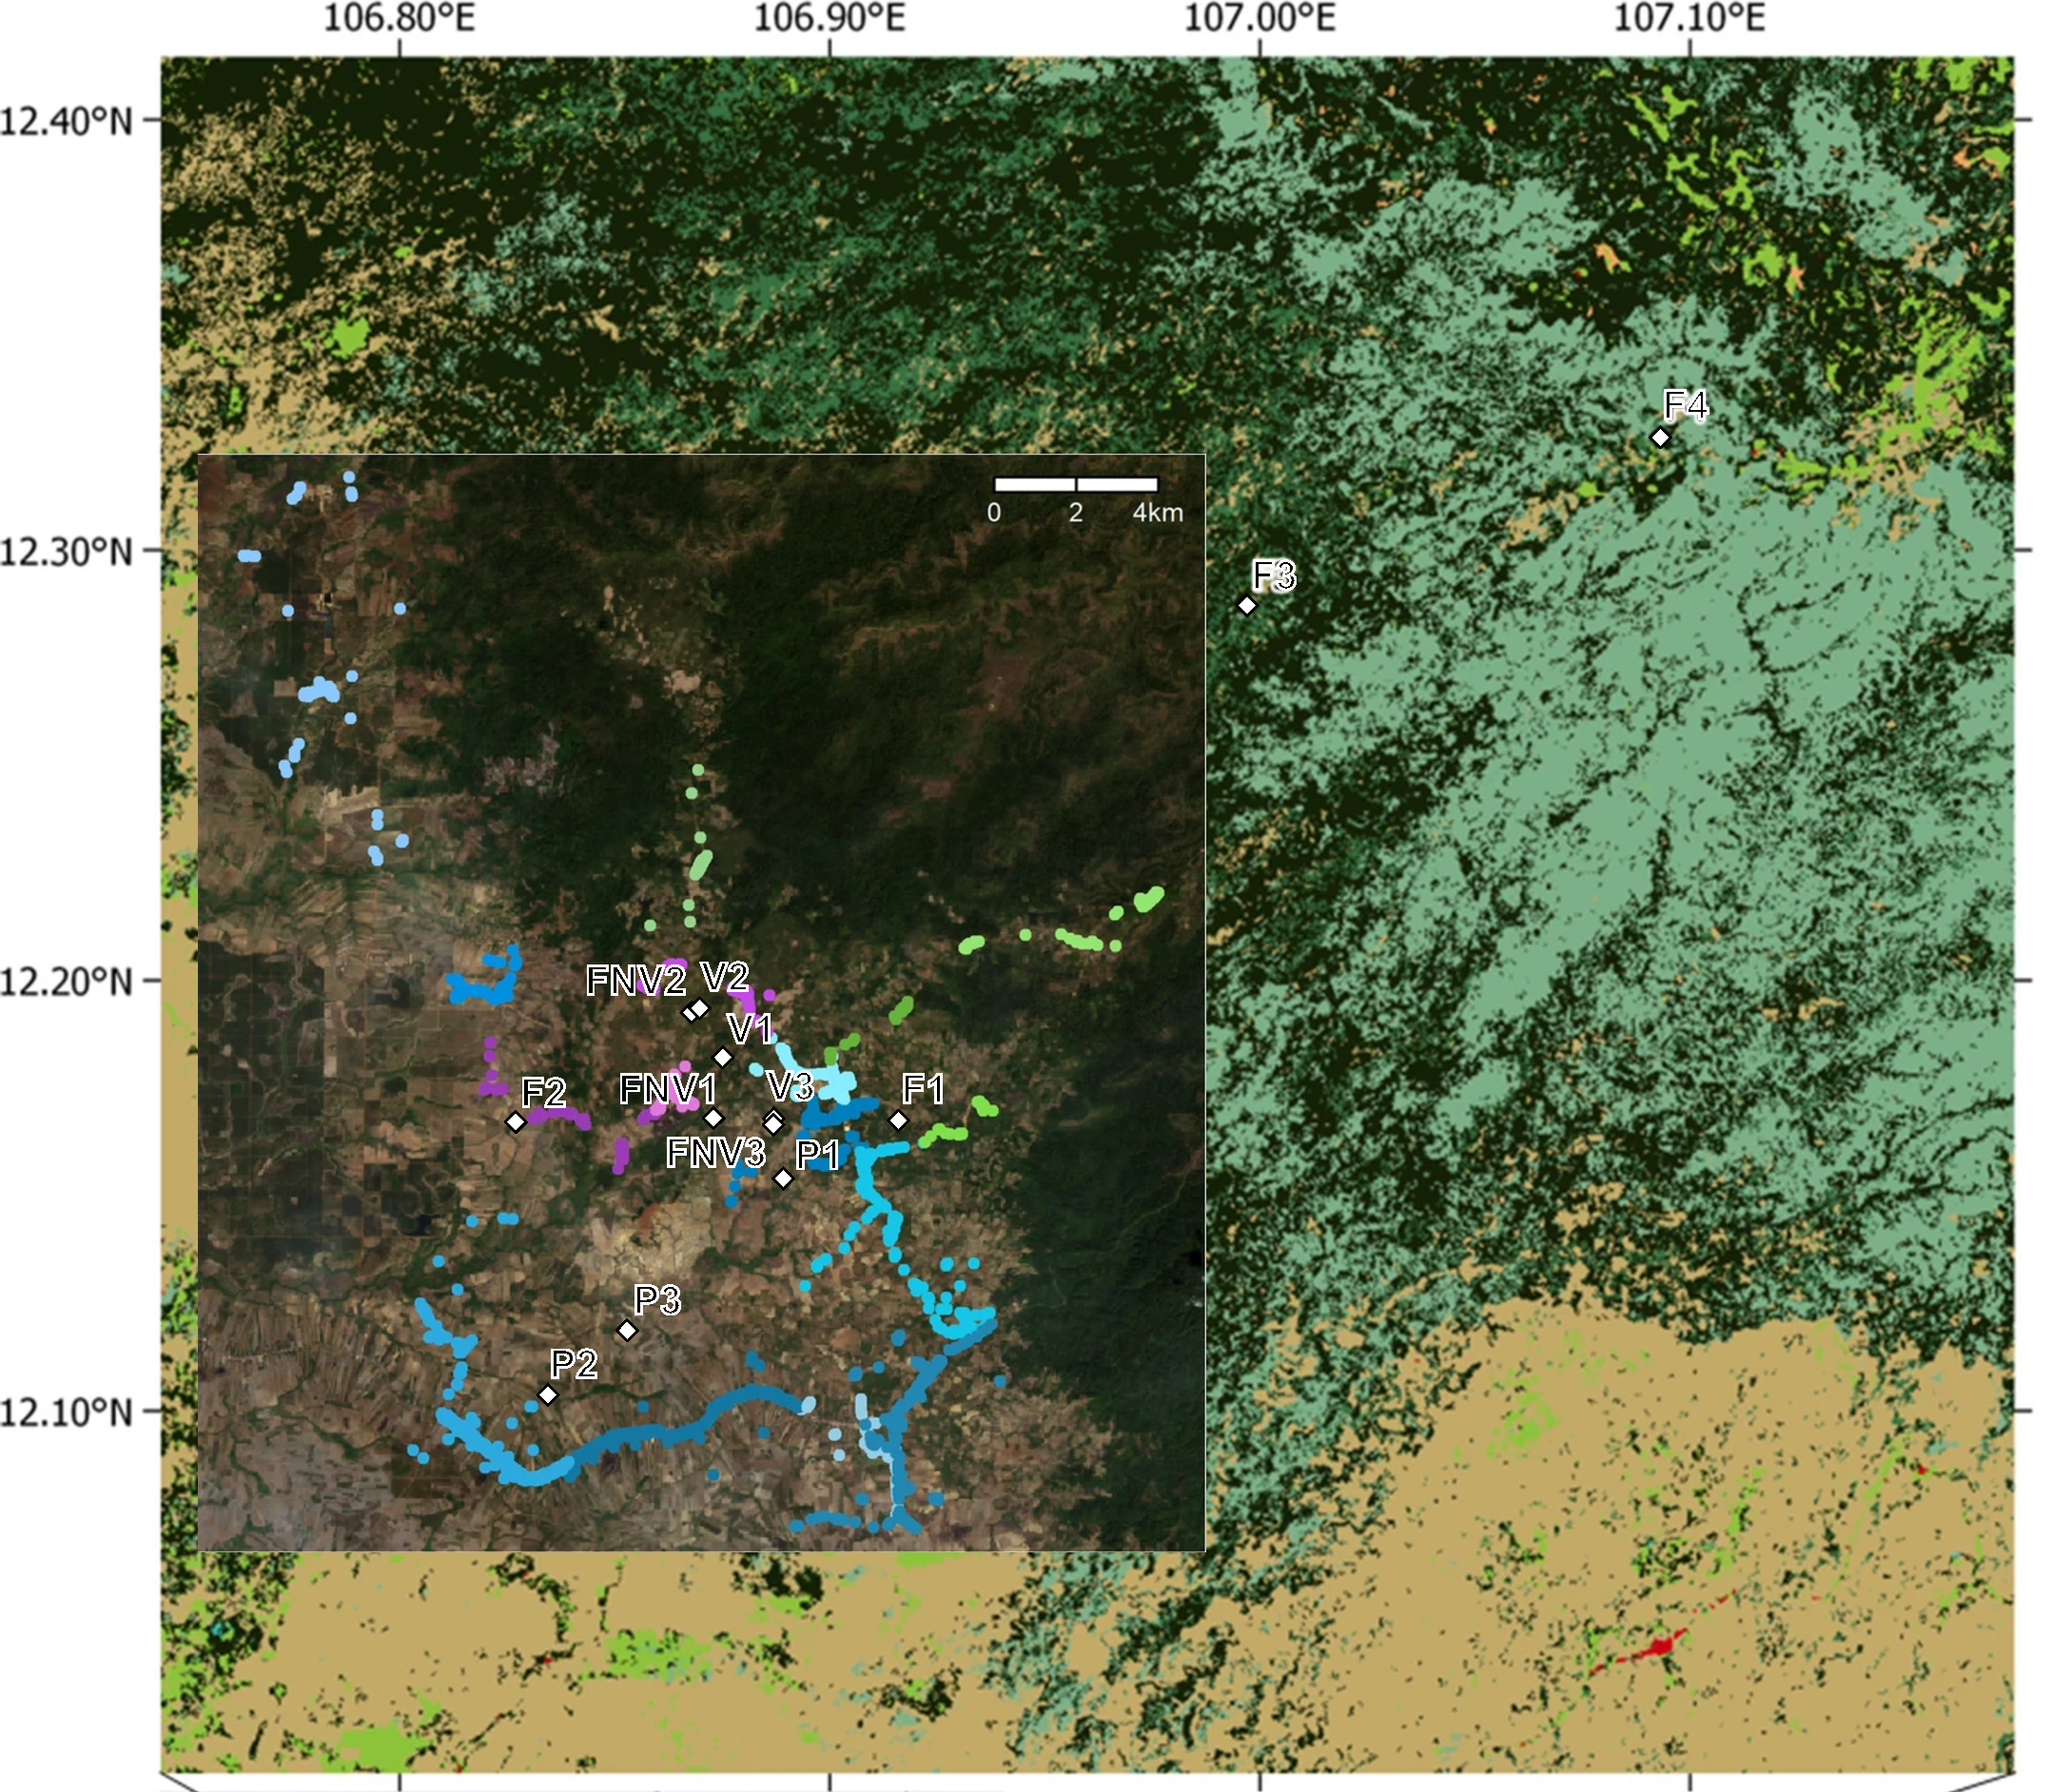
\includegraphics[width=\textwidth]{figures/ch4/collection-regions.pdf}
             \bcaption{Collection sites of mosquitoes overlayed on survey region.}{Coloured dots represent survey locations from \citet{vantaux_anopheles_2021}, whereas diamonds represent collection sites. Sites include forest locations (F1--4), forest-near-village locations (FNV1--3), villages (V1--3), and plantations (P1--3). Larger map taken from \citet{vantaux_anopheles_2021} and smaller overlaid map from \citet{sandfort_forest_2020}.}
        \label{fig:collection-sites}
    \end{figure}

    Village and plantation collection sites (V1–3, P1–3) lied in the outside forest region, whereas the forest-near-village collection sites (FNV1--3) were representative of the fringe forest region. The second forest collection site (F2) was re-classified to the fringe forest region due to its proximity to fringe forest households, and the other forest classification sites (F1, F3, F4) represented the inside forest region. Table~\ref{tab:mosquito-collection} shows the aggregation process to derive the density of mosquitoes per region.

    \begin{table}[hbt!]
        \centering
        \begin{adjustbox}{center}
            \begin{tabular}{ccccc} \toprule
                \multirow{2}{*}{Region} & \multirow{2}{*}{Site} & \multirow{2}{*}{\shortstack[c]{Mosquitoes\\collected}} & \multirow{2}{*}{\shortstack[c]{Average mosquitoes\\per site}} & \multirow{2}{*}{Density ratio} \\
                & & & & \\ \midrule
                \multirow{4}{*}{Inside forest} & F1 & 185 & \multirow{4}{*}{86.33} & \multirow{4}{*}{3.24} \\ 
                 & F3 & 53 & ~ & ~ \\ 
                 & F4 & 21 & ~ & ~ \\ 
                 & \textbf{Total} & 259 &  &  \\ \midrule
                \multirow{3}{*}{Fringe forest} & F2 & 231 & \multirow{3}{*}{78.50} & \multirow{3}{*}{2.94} \\
                 & FNV1–3 & 83 & ~ & ~ \\ 
                 & \textbf{Total} & 314 &  &  \\ \midrule
                \multirow{3}{*}{Outside forest} & V1–3 & 43 & \multirow{3}{*}{26.67} & \multirow{3}{*}{1} \\ 
                 & P1–3 & 117 & ~ & ~ \\ 
                 & \textbf{Total} & 160 &   &   \\ \bottomrule
            \end{tabular}
        \end{adjustbox}
        \bcaption{Mosquito collection site statistics and density derivation.}{Collection sites were mapped to regions and mosquito figures were aggregated. Then, densities were derived based on the average number of mosquitoes collected within the region. Data were sourced from supplementary data in \citet{vantaux_anopheles_2021}.}
        \label{tab:mosquito-collection}
    \end{table}

    The resulting ratio of mosquito densities across patches was $1 : 2.94 : 3.24$, which was rounded to $1 : 3 : 3.5$ to eliminate implausible precision. The corresponding patch carrying capacities were thus $K_v^{(1)}=3K_v^{(0)}$ and $K_v^{(2)}=3.5K_v^{(0)}$, where $k=0$ is the outside forest patch, $k=1$ is the fringe forest patch, and $k=2$ is the inside forest patch. I chose $K_v^{(0)}$ such that the extended model had the same approximate timing of peak epidemic activity as the high movement baseline scenario from \citet{manore_network-patch_2015} (approximately 100 days, as shown in Figure~\ref{fig:validation-2}). This alignment, shown in Figure~\ref{fig:k_v_candidates}, effectively calibrated the extended model to reproduce the infection dynamics of the baseline model. The resulting patch carrying capacities were $K_v^{(0)} = 2700, K_v^{(1)}= 8100, K_v^{(2)}=9450$.

    \begin{figure}[hbt!]
         \centering
         \includegraphics[width=\textwidth]{figures/ch4/k_v_candidates.pdf}
         \vspace{-1cm}
         \bcaption{Distribution of epidemic peak timings for different $K_v^{(0)}$ values.}{$K_v^{(0)}=2700$ was found to most closely align with the high movement scenario from \citet{manore_network-patch_2015} of approximately 100 days. Results from $K_v^{(0)}$ values 10\% below and above this value are shown on the left and right respectively. Median values for groups from left to right were: 102, 100, and 97 days.}
        \label{fig:k_v_candidates}
    \end{figure}
    
    \item[Heterogeneous location exposure parameters.] In the survey data, agents' exposure to mosquitoes in fields and forests was different compared to households. To capture this in the extended model, I adjusted the location exposure parameter $\alpha_j$. According to supplementary data from \citet{sandfort_forest_2020}, 57\% of participants live in households with windows, so I set $\alpha_{\text{household}}=0.43$ to capture this partial protection in most households. Field and forest work sites are entirely exposed to the outdoors, so I assumed $\alpha_{\text{field}}=\alpha_{\text{forest}}=1.0$ in the extended model.
\end{description}

\subsubsection{Indicators of model validity}\label{maiasec:questions}

To assess the validity of the extended model, I compared the observed trends in the Cambodia data to the behaviour of the extended model under similar conditions. This section in the MAIA framework proposes integrating validation into the qualitative data alignment process by identifying indicators of the extended model's usability and validity \cite{ghorbani_maia_2013}. To holistically validate the extended model's behaviour, I propose the following dynamics to be investigated later in this chapter during experimentation:

\begin{description}
    \item[Mosquito biting rates and exposure times.] Since mosquito activity is highest during the hours of dusk, nighttime, and dawn, most agents should be infected during these hours.
    \item[Heterogeneous infection risk across patches.] In \citet{vantaux_anopheles_2021}, the forest regions had six times more infectious mosquito bites compared to villages. Therefore, in the extended model, infections in the fringe and inside forest patches should be substantially higher than those in the outside forest patch.
    \item[ITNs decrease infections during the night.] Increasing $p_{\text{ITN}}$ should lead to higher ITN adoption across the province, and thus a decrease in overall transmission.
    \item[Heterogeneous occupation exposure rates.] \citet{sandfort_forest_2020} found that prevalence of malaria was highest in forest workers (25.5\%), lower in field workers (7.2\%), and lowest in non-workers (1.5\%). The risk profiles of occupations in the extended model should reflect this ordering.
\end{description}

\subsubsection{Experiments and sensitivity analysis}

I conducted various experiments and sensitivity analysis to address the validation criteria proposed in Section~\ref{maiasec:questions}. First, I ran the model 50 times with no agent ITN use ($p_{\text{ITN}}=0$) to investigate the dynamics of the parameterised extended model without interventions. Then, I visualised the behaviour of the model to investigate the validity considerations around mosquito biting rates, infection timings, infection risk, and varying risk profiles of occupational groups. Next, I varied ITN use to assess the impacts of different preventive measure compliance rates in the population. Specifically, I varied the probability an agent slept under an ITN ($p_{\text{ITN}}$) across three values: 0\%, 50\%, and 100\%. Finally, I conducted sensitivity analysis to quantify the effects of heterogeneous mosquito densities across patches by simulating three distinct scenarios:

\begin{description}
    \item[1. Derived patch carrying capacities.] I ran the model with the values for $K_v^{(0)}$, $K_v^{(1)}$, and $K_v^{(2)}$ derived using empirical data from \citet{vantaux_anopheles_2021} above.
    \item[2. Equal total volume, distributed uniformly.] Preserving the total number of mosquitoes from the derived $K_v^{(k)}$ values (i.e., $\sum_{k}{K_v^{(k)}}$), I distributed all mosquitoes over the three patches uniformly, i.e., $\forall k : K_v^{(k)}=\frac{1}{3}\sum_{k}{K_v^{(k)}}$.
    \item[3. Equal total volume, distributed with equal vector-to-host ratios.] Similar to the second scenario, using $\sum_{k}{K_v^{(k)}}$, I instead distributed mosquitoes according to the patch densities such that all patches had an equal vector-to-host ratio (i.e., $K_v^{(0)}/N^{(0)}_h=K_v^{(1)}/N^{(1)}_h=K_v^{(2)}/N^{(2)}_h$ (where $N^{(k)}_h$ denotes the number of agents belonging to the $k^{\text{th}}$ patch).
\end{description}

All other parameters used during experiments which were not derived in the previous sections remained the same as in the baseline model (see Appendix~\ref{appendix:manore-abm} for reference).

\subsection{Results}\label{sec:extended-model-results}

In this section, I present the results from the experiments described above. First, I describe the default behaviour of the model over 50 simulations without any variation in parameters. The purpose of this is to validate whether the expected dynamics described in Section~\ref{maiasec:questions} were observed when running the extended model. Next, I discuss the impacts of varying ITN adoption ($p_{\textsc{ITN}}$) of agents within the extended model. Finally, I investigate how heterogeneous mosquito densities across patches ($K_v$) affected disease spread.

\subsubsection{Validation of extended model}\label{sec:extended-model-validation}

\begin{figure}[htb!]
     \centering
     \includegraphics[width=.9\textwidth]{figures/ch4/no_itn_disease_dynamics.pdf}
     \bcaption{Agent disease dynamics over time.}{Solid lines represent results from the most representative model run\protect\footnotemark. Shaded bands around lines represent minimum and maximum values across all model runs\protect\footnotemark.}
    \label{fig:ch4res-overall}
\end{figure}

\newcounter{savefootnote}% Ensure the savefootnote counter exists

\setcounter{savefootnote}{\value{footnote}}% Store footnote counter
\addtocounter{footnote}{-1}% Decrease the footnote counter by 1
\footnotetext{I determine the most representative model run by choosing the result that minimises the sum of Euclidean distances across all other model runs.}

\setcounter{footnote}{\value{savefootnote}}% Restore the footnote counter
\footnotetext{Shaded bands around solid lines represent minimum and maximum values across all model runs in all other figures throughout this thesis, unless explicitly stated otherwise.}

Across the 50 model runs without any variation in parameters, $92.8\% \pm 0.5\%$ of agents were infected with disease, on average. Figure~\ref{fig:ch4res-overall} demonstrates the agent SIR dynamics across all model runs. Mosquito dynamics were heterogeneous across patches due to variable vector-to-host ratios, as shown in Figure~\ref{fig:ch4res-mosquito-dynamics}. Infection in the outside forest patch peaked the latest compared to the fringe and inside forest patch due to the low density of mosquitoes relative to a large (85\% of total) host population. Unlike the outside forest patch, the fringe and inside forest patches had steepened infection curves, and as a consequence, higher forces of infection on mosquitoes ($\lambda_v$) during the day and night. Unsurprisingly, nighttime $\lambda_v$ values were consistently higher than their daytime values due to heightened mosquito activity which caused higher biting rates, and thus a higher chance of mosquito infection during the hours of dusk, nighttime, and dawn.

\begin{figure}[hbtp!]
     \centering
     \adjustbox{width=1.1\textwidth,center}{%
        \includegraphics{figures/ch4/no_itn_mosquito_dynamics.pdf}
     }
     \bcaption{Mosquito disease dynamics across patches over time.}{SEI dynamics for mosquitoes are shown in the top row. Forces of infection on vectors ($\lambda_v$) are shown on the bottom row. Nighttime (when mosquito activity is heightened by 4x) forces of infection were always higher than daytime values. Because the outside forest patch did not quickly reach infection saturation, dynamics are spread out over the 200-day time frame.}
    \label{fig:ch4res-mosquito-dynamics}
\end{figure}

\begin{figure}[htb!]
     \centering
     \includegraphics[width=.9\textwidth]{figures/ch4/no_itn_cum_infected_agents.pdf}
     \bcaption{Cumulative infected agents across patches.}{Compared to the slower progression of the outside forest patch, the fringe and inside forest patches reached saturating levels of infection by day 60--65 due to their high vector-to-host density ratios.}
    \label{fig:ch4res-cum-infections}
\end{figure}

\begin{figure}[htb!]
     \centering
     \adjustbox{width=1.1\textwidth,center}{%
        \includegraphics{figures/ch4/no_itn_freq_infection.pdf}
    }
     \bcaption{Frequency of infection times and biting rates.}{Infection times (blue bars) were aggregated across all model runs and are shown in 24-hour format. Biting rates (black lines) are shown for one model run as the variation in biting rates was minimal. Values are highest when agents are exposed (at work) and mosquito activity is heightened by 4x during 6pm--10am.}
    \label{fig:ch4res-infection-day}
\end{figure}

\begin{figure}[hbt!]
     \centering
     \includegraphics[width=0.85\textwidth]{figures/ch4/no_itn_agent_infection_cum_occupation.pdf}
     \bcaption{Proportion of infected agents over time by occupation.}{\textbf{(i)} Infection proportions per risk group. \textbf{(ii)} Cumulative infection proportions per risk group. Forest workers reached saturating infection levels quickly due to their constant high exposure to mosquitoes. Field workers were more exposed to mosquitoes than non-workers, and thus experienced slightly higher rates of infection.}
    \label{fig:ch4res-risk-profiles}
\end{figure}

One interesting result was that the highest-risk inside forest patch had lower nighttime $\lambda_v$ values compared to the fringe forest patch. This was due to the patch's slightly smaller host population, a lower proportion of fully exposed workers, and the fact that forest workers tend to live in the outside or fringe forest patches, meaning they leave the inside forest patch to return home after work, reducing the concentration of infected agents in the patch, thus lowering $\lambda_v$. As shown in Figure~\ref{fig:ch4res-cum-infections}, infections across the fringe and inside forest patches typically saturated the host populations quickly in comparison to the slower rate of agent infection within the outside forest patch.

In the simulation, infection risk was also heterogeneous according to the time of day. Figure~\ref{fig:ch4res-infection-day} conveys how the 4x heightened mosquito activity during dusk, nighttime and dawn led to increased biting rates across all patches, disproportionately affecting the fringe and inside forest patches due to their high mosquito density. As a result of higher biting rates, agent infection mostly occurred in the late afternoon to early morning, and was most prevalent when mosquitoes were more active but agents were still at work (8--10am and 6--8pm). This high prevalence of infection during the nighttime despite protection from indoor household environments highlights the importance of vector control tools that limit contact rates during this time (such as ITNs).

\begin{figure}[hbt!]
     \centering
     \includegraphics[width=0.8\textwidth]{figures/ch4/no_itn_exposure_location.pdf}
     \bcaption{Frequency of agent infection locations by occupation.}{Infection counts in locations are aggregated across all model runs. Almost all forest workers were exposed at forest sites, compared to field workers who were mostly exposed at home. Non-workers were only ever exposed at home.}
    \label{fig:ch4res-inf-locations}
\end{figure}

Disease transmission was significantly different across agent occupations. Forest workers were consistently fully infected before halfway through the simulation, whereas infections for field and non-workers typically plateaued by the end of the simulation. As evidenced by Figure~\ref{fig:ch4res-risk-profiles}, the higher mosquito exposure of field workers led to a higher average infection count compared to the non-working population. Despite their frequent exposure to mosquitoes, most field workers (55.3\%) were infected while sleeping at home instead of within a field work site (38.1\%), as shown in Figure~\ref{fig:ch4res-inf-locations}. Forest workers, on the other hand, were overwhelmingly infected in their place of work (89.0\%) compared to their households (10.5\%)\footnote{These proportions suggest that across all model runs, only 0.5\% of forest workers remained uninfected by the end of the simulation.}.

\subsubsection{Impacts of preventive measure adoption}\label{sec:extended-model-p-itn-impacts}

\begin{figure}[htb!]
     \centering
     \includegraphics[width=0.85\textwidth]{figures/ch4/itn_agent_infection_p_use.pdf}
     \bcaption{Proportion of agents infected over time for different levels of ITN use.}{\textbf{(i)} Proportion of agents infected over time. \textbf{(ii)} Cumulative proportion of agents infected over time. Although no level of ITN adoption led to disease eradication, increasing ITN adoption from 0\% to 50\% led to a 15--20\% decrease in total infections on average, while 100\% adoption rates significantly reduced total infection counts to $<$40\% in all runs.}
    \label{fig:ch4res-itn-dynamics}
\end{figure}

\begin{figure}[htb!]
     \centering
     \adjustbox{width=1.2\textwidth,center}{%
        \includegraphics{figures/ch4/itn_risk_groups.pdf}
    }
     \bcaption{ITN use impacts on infected agents by occupation.}{The top row conveys infections over time, whereas the bottom row shows cumulative infections within each occupation. Forest workers were the least affected by ITN use due to their exposure, while field and non-workers greatly benefitted from adopting ITNs, approximately halving disease cases in both occupational groups.}
    \label{fig:ch4res-inf-occupations}
\end{figure}

As expected, ITN use drastically decreased disease spread. As shown in Figure~\ref{fig:ch4res-itn-dynamics}, increasing ITN use delayed the first peak of disease spread and flattened the second wave of disease. In the complete compliance case ($p_{\text{ITN}}=1.0$), ITNs reduced infection counts across simulations to under 40\% (from $>90\%$) and prevented the momentum of the first wave of disease from leading to a severe second wave, as in the 0\% and 50\% ITN adoption scenarios. That being said, all three scenarios of ITN use had an initial peak in infections between days 50--100.

\begin{figure}[htb!]
     \centering
     \adjustbox{width=1.2\textwidth,center}{%
        \includegraphics{figures/ch4/itn_freq_infection.pdf}
    }
     \bcaption{Frequency of infection times across ITN adoption rates.}{Infection times were aggregated across all model runs and are shown in 24-hour format. As ITN adoption increased, infections were concentrated during daytime hours of exposure.}
    \label{fig:ch4res-itn-infection-day}
\end{figure}

\begin{figure}[htb!]
     \centering
     \adjustbox{width=1.3\textwidth,center}{%
        \includegraphics{figures/ch4/itn_exposure_locations.pdf}
    }
     \bcaption{Agent exposure locations by risk group and ITN adoption.}{Infection counts in locations were aggregated across all model runs. As ITN adoption increased, field workers and non-workers experienced less infections at home, but forest workers remained relatively unaffected.}
    \label{fig:ch4res-itn-locations}
\end{figure}

The breakdown of infections by occupations in Figure~\ref{fig:ch4res-inf-occupations} demonstrates that these early peaks were due in part to the rapid infection of forest workers. When ITN use was increased, the rate of infection among field and non-workers was substantially lower, however the working population in the forest was relatively unaffected. This is not surprising given that forest workers were rarely infected in their households as shown in Figure~\ref{fig:ch4res-inf-locations}, so the impact of using ITNs was understandably diminished compared to field and non-workers.
% due to the single forest site location in the high-risk inside forest patch. 

Increasing ITN use led to higher daytime infection rates and more concentrated disease spread within work site locations. Figure~\ref{fig:ch4res-itn-infection-day} shows how increasing ITN use decreased infection during nighttime hours but concentrated disease spread during the daytime. Notably, infections grew most in the early morning and late afternoon hours compared to the relatively stable (but increasing) infections within mid-late daytime hours. Corresponding with the decrease in nighttime infections, agents were less likely to be infected in households as ITN use increased. As shown in Figure~\ref{fig:ch4res-itn-locations}, non-worker infections dropped from 89.0\% with no ITN use to 25.5\% in the total compliance scenario. Field workers similarly saw infections drop from 55.4\% without ITN use to 34.1\% in the half compliance scenario, and virtually no infections occurred within households in the full compliance case. As noted earlier, however, forest workers benefitted the least from ITNs, as only 10.5\% of forest worker infections originally occurred in households.


\subsubsection{Impacts of heterogeneous mosquito densities}

\begin{figure}[htb!]
     \centering
     \adjustbox{width=0.9\textwidth,center}{%
        \includegraphics{figures/ch4/k_v_distribution_epidemic_peak.pdf}
    }
     \bcaption{Distribution of epidemic peak timings across patch carrying capacity scenarios.}{\q{Derived} indicates the empirically derived carrying capacity values, whereas the two \q{equal} experiments are more homogeneous across patches. As mosquito distribution was more equal across patches, so were epidemic dynamics.}
    \label{fig:ch4-k-v-timings}
\end{figure}

\begin{table}[htb!]
    \centering
    \begin{adjustbox}{center}
        \begin{tabular}{ccccccc} \toprule
            \multirow{2}{*}{Scenario} & \multirow{2}{*}{$K_v^{(0)}$} & \multirow{2}{*}{$K_v^{(1)}$} & \multirow{2}{*}{$K_v^{(2)}$} & \multirow{2}{*}{$\sum_k{K_v^{(k)}}$} & \multirow{2}{*}{\shortstack[c]{Arithmetic mean of total agents\\infected by simulation end (/10,053)}} & \multirow{2}{*}{\shortstack[c]{Standard\\deviation}} \\
            {} & {} & {} & {} & {} & {} & {} \\ \midrule
            Derived values & 2,700 & 8,100 & 9,450 & 20,250 & 9,324.7 & 47.5 \\[.25cm]
            Equal (volume) & 6,750 & 6,750 & 6,750 & 20,250 & 9,998.5 & 7.4 \\[.25cm]
            Equal (ratio) & 17,212.5 & 1,620 & 1,417.5 & 20,250 & 10,051.05 & 1.3 \\ \bottomrule
        \end{tabular}
    \end{adjustbox}
    \bcaption{Impacts of heterogeneity in mosquito patch carrying capacities.}{Results were aggregated over 20 model runs per scenario. Derived values used carrying capacities calculated from empirical data in Section~\ref{ch4:parameterisation}. Equal (volume) values were computed by uniformly distributing the sum of derived values over three patches. Equal (ratio) values were spread according to values that led to an equal vector-to-host ratio in all patches ($\approx2$).}
    \label{tab:ch4-k_v}
\end{table}

As was the case in the baseline model, heterogeneous mosquito densities across patches substantially impacted disease spread among agents. Table~\ref{tab:ch4-k_v} lists the scenarios simulated to assess the impacts of patch heterogeneity on the extended model and the resulting average number of agents infected by the end of the simulation. As carrying capacities across patches became more \q{equal} (first in terms of volume, then vector-to-host ratios), infection in agents increased and became less variable. This was expected since both alternative parameterisations increased the outside patch carrying capacity ($K_v^{(0)}$), leading to a larger force of infection on agents in the most populous patch, thereby accelerating disease spread.

As patches became homogeneous in mosquito density, so did their infection risk profiles. As shown in Figure~\ref{fig:ch4-k-v-timings}, while the timing of epidemic peaks for the outside forest patch were initially distinct from the fringe and inside forest patches, increasing homogeneity in mosquito densities across patches centred the distributions of epidemic peak timings. This was replicated for infection dynamics, where infections peaked early on in the equal scenarios, rather than twice over the course of the simulation (as shown in Supplementary Figure~\ref{fig:ch4-k-v-infs}). Overall, as expected, cumulative infections across the three patches homogenised as mosquito densities became equal (shown explicitly in Supplementary Figure~\ref{fig:ch4-k-v-patch-infs}).


\subsection{Discussion}\label{sec:extended-model-discussion}

By using survey data collected in the Mondulkiri province, the parameterisation and extensions to the baseline model served to represent a real-world setting and empirically ground the dynamics of the extended model. In this chapter, I investigated the research aims established earlier---to align the extended model to a realistic setting, and to assess impacts of preventive measures---by simulating hypothetical scenarios within the extended model and quantifying the effects of preventive measure use. Below, I discuss the progress made towards these aims and conclude with the limitations of the extended model.

\subsubsection{Extended model validation and evaluation}\label{sec:extended-model-validation-results}

Overall, the results conveyed above demonstrate an alignment of the extended model with the observations in \citet{sandfort_forest_2020, pepey_mobility_2022, vantaux_anopheles_2021}. First, mosquito biting rates and exposure times were heterogeneous over time due to the mechanism of increasing $\sigma_v$ outside of daytime hours. As expected, this led to higher infection rates for agents during the night despite protection from household dwellings. Second, infection risk across patches was heterogeneous in the model, as in the survey data. Disease was more prevalent in the fringe and inside forest patches due to higher mosquito densities compared to the village (outside forest patch), which aligned with findings from \citet{sandfort_forest_2020, vantaux_anopheles_2021}. 

Interestingly, nighttime forces of infection on vectors were lower in the inside forest patch than the fringe forest patch, despite the former patch having a higher mosquito density. As explained, this was due to a smaller working population within the patch and the regular outbound travel of infectious forest workers from the patch at the end of the workday. Although no data exist to confirm this finding with empirical observations from the province, this emergent dynamic in the model highlights the importance of understanding occupational mobility across regions.

Agent occupations were also heterogeneously exposed to disease, with the expected ordering observed in the data (forest workers were at highest risk of infection, then field workers, and finally non-workers). Since forest workers do not necessarily live in the inside forest patch, the workers that travel home to other patches after work carry the disease with them, spreading infection through regular mobility patterns. This is consistent with findings from \citet{sandfort_forest_2020} in which travel and work trips into the forest were \q{particularly strong risk factors} for malaria, alongside proximity to the forest. As \citet{sandfort_forest_2020} additionally noted, \q{infection risk is less confined to forest-goers in sub-populations that already live in forested areas and suggests within-village transmission.}

Forest workers reacted distinctly when ITN use was varied within the population. When ITN adoption was increased, infection within field and non-workers dropped substantially. However, the reduction in disease spread for forest workers was minimal, suggesting ITNs are not an effective preventive measure for reducing disease spread in the sub-population. \citet{sandfort_forest_2020} echoed this sentiment in the context of the Cambodian region, stating that \q{a focus of interventions solely on forest-goers could ... be insufficient to reach the goal of nation-wide malaria elimination.}

Overall, these results indicate that the extended model can reproduce the core dynamics observed within the real-world data, and the impacts of preventive measure use on disease spread are thus aligned to a realistic setting. As the model incorporates a validated dimension of realism, the overarching research question of this thesis can subsequently be investigated by extending this model with behaviour change theories in the following chapter.


\subsubsection{Limitations and assumptions}

Despite the alignment of the extended model to the survey data, there are a number of limitations to the model. One major limitation is that agent mobility is crudely simplified: Movement between locations does not take into account exposure during travel, which was a significant factor for malaria risk in the survey data, with examples of high-risk travel including overnight trips to the forest \cite{sandfort_forest_2020}. These overnight trips to the forest would likely be catalysts for disease spread as they take place during peak mosquito activity hours, but because the extended model assumes work only occurs in the daytime, this risk is not represented in the model. Additionally, the choice of three occupations in the extended model means risk groups other than forest workers are not regularly exposed to the forest. This is contrary to findings from \citet{sandfort_forest_2020}, in which travels into the forest \q{actually extend[ed] to a much broader range of the population} (e.g., non-working women and children).

Furthermore, the model architecture adopted from \citet{manore_network-patch_2015} also imposes additional limitations on the extended model. For example, the groupings of households into patches conducted in Section~\ref{sec:ch4-extensions} excludes the possibility of household-household disease spread in the model, which was an observed form of local heterogeneity \cite{pepey_mobility_2022}. Furthermore, all agents are assumed to have unimpeded access to ITNs with a consistently high efficacy, which is an unrealistic assumption since ITN quality typically degrades over time \cite{manuv_investigating_2023}. While these drawbacks of the model are not insignificant, they are arguably necessary limitations to accept in order to make simplifying assumptions of the complexities of the Mondulkiri province. While I purposefully simplify these mechanisms in the extended model, in later chapters I suggest directions for future work that may be able to incorporate these additional relationships.
\clearpage

\section{Implementing behaviour change theories}\label{sec:bcts}

In this chapter, I design, implement, and parameterise two behaviour change theories (BCTs) within the extended model from the previous chapter. Specifically, I address how integrating theories from psychology into computational models can affect dynamics of disease spread and preventive behaviours. To do so, I adapt and propose methodologies for integrating two distinct BCTs within an agent-based model (ABM), and I investigate the similarities and differences of these implementations. This chapter therefore completes Objectives~\ref{ro3}--\ref{ro5} set out in Section~\ref{sec:research-aims}, laying the foundation for the following chapter which synthesises results from the baseline model, the extended model, and the integration of BCTs.

The structure of this chapter is as follows: First, I explain the importance of psychological BCTs in the context of vector-borne disease (VBD) spread and discuss prior attempts to integrate BCTs within ABMs. Then, I detail my computational implementations of the two BCTs in the extended model. Finally, I assess the impacts of integrating BCTs through two hypothetical scenarios and sensitivity analysis, and I conclude by discussing the implications of my findings within epidemiological and computational modelling contexts.

\subsection{Psychological behaviour change theories}

Psychological BCTs propose mechanisms for why individuals change their behaviour, and as a result, can explain the preventive behaviours of populations. As outlined in greater detail in Section~\ref{sec:lit-review-bcts}, BCTs draw on socio-psychological phenomena to define \textit{constructs}---contextual and personal factors of individuals that combine to explain individual behaviours. In VBD contexts, self-protection is typically a voluntary action involving the use of preventive measures, such as sleeping under insecticide-treated bed nets (ITNs) or applying mosquito repellent. Therefore, understanding the individual factors that drive preventive behaviours within at-risk populations is crucial not only for forecasting disease spread, but also for designing effective health interventions to motivate preventive measure use \cite{vande_velde_integrated_2024}. For these reasons, integrating theories of behaviour change into computational models of disease spread presents an opportunity to explore how preventive behaviours may evolve when grounded in socio-psychological frameworks.

Integrating BCTs into ABMs can create nuanced representations of behaviour and enrich models with emergent, evolving patterns of preventive behaviours. Previous studies have formalised and incorporated BCTs into ABMs to examine how dynamic agent decision-making influences disease spread \cite{durham_incorporating_2012, abdulkareem_risk_2020, weston_infection_2018, bedson_review_2021}. Successful efforts, such as those by \citet{durham_incorporating_2012} and \citet{kurchyna_seeing_2024}, have demonstrated the utility of integrating BCTs for providing mechanistic explanations of preventive behaviour dynamics. Because BCTs are formulated from the perspective of individuals, they are inherently aligned with the agent-based approach. The main challenge, however, lies in translating these theoretical frameworks into computational ones \cite{durham_incorporating_2012}. Despite this, prior research provides a strong foundation for adapting and integrating the two BCTs examined in this thesis into the extended model of VBD spread presented in Chapter~\ref{sec:extended_model}.

\begin{figure}[htbp]
     \centering
     \vspace{.5cm}
     \begin{subfigure}[b]{\textwidth}
         \centering
         \begin{adjustbox}{center}
              \includegraphics[width=1\textwidth]{figures/ch5/hbm-conceptual-diagram.pdf}
         \end{adjustbox}
         \caption{\textbf{Health Belief Model}}
         \label{fig:hbm-conceptual-comparison}
     \end{subfigure}%
     \\ \vspace{1cm}
     \begin{subfigure}[b]{\textwidth}
         \centering
         \begin{adjustbox}{center}
            \includegraphics[width=1.2\textwidth]{figures/ch5/pmt-conceptual-diagram.pdf}
         \end{adjustbox}
         \caption{\textbf{Protection Motivation Theory}}
         \label{fig:pmt-conceptual-comparison}
     \end{subfigure}
    \bcaption{Conceptual formulations of chosen behaviour change theories.}{\textbf{(i)} HBM, adapted from \citet{champion_health_2015}. \textbf{(ii)} PMT, adapted from \citet{norman_protection_2015}. Re-displayed here from Figures~\ref{fig:lit-review-hbm} and \ref{fig:lit-review-pmt} for convenience.}
    \label{fig:bct-conceptual-comparison}
\end{figure}

I adapt the extended model to include computational formulations of the Health Belief Model (HBM) and Protection Motivation Theory (PMT). These two BCTs are particularly suited for this research for the following reasons: First, while many BCTs can be applied to protective health behaviours \cite{vande_velde_integrated_2024}, both the HBM and PMT have frequently been used in studies relating to VBD spread (e.g., \cite{watanabe_determinants_2014, yirsaw_insecticide-treated_2021, donohoe_tick-borne_2018} for the HBM; \cite{ghahremani_effect_2014} for PMT). Second, as shown in Figure~\ref{fig:bct-conceptual-comparison}, both BCTs share relatively simple and comparable structures, with overlapping constructs related to the perceived severity and susceptibility to a disease, and the perceived benefits of---and barriers to---adopting a preventive measure \cite{marikyan_protection_2023, weinstein_testing_1993, champion_health_2015}. Lastly, mathematical formulations for both theories already exist, and have been specifically designed for integration within ABMs \cite{durham_incorporating_2012,kurchyna_seeing_2024}.

In the next section, I draw on work from \citet{durham_incorporating_2012} and \citet{kurchyna_seeing_2024} to integrate the HBM and PMT into the extended model presented in Chapter~\ref{sec:extended_model}. Instead of assuming fixed proportions of ITN adoption, as in the previous chapter, I use the integrated BCTs to dynamically determine whether agents sleep under ITNs. I then create three experiments to explore how this dynamic decision-making process impacts preventive behaviours and disease spread under each BCT.

\subsection{Methods}

In this section, I describe the integration of the two chosen BCTs---the HBM and PMT---into the extended model. First, I outline the computational formulations of each theory and explain how they are parameterised to the context of ITN use using VBD survey data. Then, I describe the experiments to investigate seasonal VBD risk before comparing the impacts of the two BCTs on the dynamics of preventive behaviours and disease spread.

\subsubsection{Health Belief Model implementation}

\begin{figure}[hbt!]
     \centering
     \begin{adjustbox}{center}
         % \includegraphics[width=1.2\textwidth]{figures/ch5/hbm-conceptual-diagram.pdf}
         % \includegraphics[width=1\textwidth]{figures/ch5/pmt-conceptual-diagram.pdf}
         \resizebox{1\textwidth}{!}{
            %% Creator: Inkscape 1.3.2 (091e20e, 2023-11-25), www.inkscape.org
%% PDF/EPS/PS + LaTeX output extension by Johan Engelen, 2010
%% Accompanies image file 'figures/ch5/hbm-math-diagram.pdf' (pdf, eps, ps)
%%
%% To include the image in your LaTeX document, write
%%   \input{<filename>.pdf_tex}
%%  instead of
%%   \includegraphics{<filename>.pdf}
%% To scale the image, write
%%   \def\svgwidth{<desired width>}
%%   \input{<filename>.pdf_tex}
%%  instead of
%%   \includegraphics[width=<desired width>]{<filename>.pdf}
%%
%% Images with a different path to the parent latex file can
%% be accessed with the `import' package (which may need to be
%% installed) using
%%   \usepackage{import}
%% in the preamble, and then including the image with
%%   \import{<path to file>}{<filename>.pdf_tex}
%% Alternatively, one can specify
%%   \graphicspath{{<path to file>/}}
%% 
%% For more information, please see info/svg-inkscape on CTAN:
%%   http://tug.ctan.org/tex-archive/info/svg-inkscape
%%
\begingroup%
  \makeatletter%
  \providecommand\color[2][]{%
    \errmessage{(Inkscape) Color is used for the text in Inkscape, but the package 'color.sty' is not loaded}%
    \renewcommand\color[2][]{}%
  }%
  \providecommand\transparent[1]{%
    \errmessage{(Inkscape) Transparency is used (non-zero) for the text in Inkscape, but the package 'transparent.sty' is not loaded}%
    \renewcommand\transparent[1]{}%
  }%
  \providecommand\rotatebox[2]{#2}%
  \newcommand*\fsize{8 pt\relax}%
  \newcommand*\lineheight[1]{\fontsize{\fsize}{#1\fsize}\selectfont}%
  \ifx\svgwidth\undefined%
    \setlength{\unitlength}{263.77443695bp}%
    \ifx\svgscale\undefined%
      \relax%
    \else%
      \setlength{\unitlength}{\unitlength * \real{\svgscale}}%
    \fi%
  \else%
    \setlength{\unitlength}{\svgwidth}%
  \fi%
  \global\let\svgwidth\undefined%
  \global\let\svgscale\undefined%
  \makeatother%
  \begin{picture}(1,0.56827175)%
    \lineheight{1}%
    \setlength\tabcolsep{0pt}%
    \put(0,0){\includegraphics[width=\unitlength,page=1]{figures/ch5/hbm-math-diagram.pdf}}%
    \put(-0.00172156,0.5140235){\color{black}\makebox(0,0)[lt]{\lineheight{1.25}\smash{\begin{tabular}[t]{l}$i=1$\end{tabular}}}}%
    \put(-0.00172156,0.40289279){\color[rgb]{0,0,0}\makebox(0,0)[lt]{\lineheight{1.25}\smash{\begin{tabular}[t]{l}$i=2$\end{tabular}}}}%
    \put(-0.00172156,0.30206003){\color[rgb]{0,0,0}\makebox(0,0)[lt]{\lineheight{1.25}\smash{\begin{tabular}[t]{l}$i=3$\end{tabular}}}}%
    \put(0.5337258,0.30917476){\color[rgb]{0,0,0}\makebox(0,0)[lt]{\lineheight{1.25}\smash{\begin{tabular}[t]{l}$\frac{\text{OR}_0\cdot\text{OR}_2\cdot\text{OR}_4\cdot\text{OR}_5}{1+\text{OR}_0\cdot\text{OR}_2\cdot\text{OR}_4\cdot\text{OR}_5}$\end{tabular}}}}%
    \put(0.33796707,0.5315256){\color{gray}\makebox(0,0)[lt]{\lineheight{1.25}\smash{\begin{tabular}[t]{l}$\text{OR}_1$\end{tabular}}}}%
    \put(0.33796707,0.41880345){\color[rgb]{0,0,0}\makebox(0,0)[lt]{\lineheight{1.25}\smash{\begin{tabular}[t]{l}$\text{OR}_2$\end{tabular}}}}%
    \put(0.33796707,0.22866551){\color[rgb]{0,0,0}\makebox(0,0)[lt]{\lineheight{1.25}\smash{\begin{tabular}[t]{l}$\text{OR}_4$\end{tabular}}}}%
    \put(0.33796707,0.13841411){\color[rgb]{0,0,0}\makebox(0,0)[lt]{\lineheight{1.25}\smash{\begin{tabular}[t]{l}$\text{OR}_5$\end{tabular}}}}%
    \put(0.33796707,0.04634328){\color{gray}\makebox(0,0)[lt]{\lineheight{1.25}\smash{\begin{tabular}[t]{l}$\text{OR}_6$\end{tabular}}}}%
    \put(0.65282162,0.12058035){\color[rgb]{0,0,0}\makebox(0,0)[lt]{\lineheight{1.25}\smash{\begin{tabular}[t]{l}$\text{OR}_0$\end{tabular}}}}%
    \put(-0.00172156,0.21152521){\color[rgb]{0,0,0}\makebox(0,0)[lt]{\lineheight{1.25}\smash{\begin{tabular}[t]{l}$i=4$\end{tabular}}}}%
    \put(-0.00172156,0.12099039){\color[rgb]{0,0,0}\makebox(0,0)[lt]{\lineheight{1.25}\smash{\begin{tabular}[t]{l}$i=5$\end{tabular}}}}%
    \put(0,0){\includegraphics[width=\unitlength,page=2]{figures/ch5/hbm-math-diagram.pdf}}%
    \put(-0.00147328,0.03045556){\color[rgb]{0,0,0}\makebox(0,0)[lt]{\lineheight{1.25}\smash{\begin{tabular}[t]{l}$i=6$\end{tabular}}}}%
    \put(0.33796707,0.31878911){\color{gray}\makebox(0,0)[lt]{\lineheight{1.25}\smash{\begin{tabular}[t]{l}$\text{OR}_3$\end{tabular}}}}%
    \put(0.92511069,0.30484217){\color[rgb]{0,0,0}\makebox(0,0)[lt]{\lineheight{1.25}\smash{\begin{tabular}[t]{l}$p_{\text{ITN}}$\end{tabular}}}}%
  \end{picture}%
\endgroup%

         }
     \end{adjustbox}
         \bcaption{HBM implementation.}{Odds ratios for constructs in a \q{high} state undergo a logistic transformation to calculate the probability of ITN use, $p_{\text{ITN}}$. Constructs in \q{low} states are greyed out (in this case, $i=1,3,6$) and their odds ratios do not contribute to the derivation of $p_{\text{ITN}}$.}
    \label{fig:hbm-implementation}
\end{figure}

I build on work by \citet{durham_incorporating_2012} to integrate the HBM into the extended model using a mathematical representation of the HBM. As shown in Figure~\ref{fig:hbm-implementation}, this formulation calculates the probability of an agent performing the preventive behaviour by combining odds ratios that map to HBM constructs. In my case, the probability that an agent uses an ITN, $p_{\text{ITN}}$, is calculated as:

\begin{equation}\label{eq:prob-hbm}
    p_{\text{ITN}} = \frac{\text{OR}_0\cdot\prod_i{\text{OR}_i^{x_i}}}{1+\text{OR}_0\cdot\prod_i{\text{OR}_i^{x_i}}},
\end{equation}
where each HBM construct is denoted by an index $i\in1,\dots,6$ (or construct names are equivalently used), where $x_i$ is the corresponding indicator variable representing the state of the construct---a \q{high} construct state is defined as $x_i=1$, whereas \q{low} is $x_i=0$. Each term $\text{OR}_{i}$ denotes the odds ratio\footnote{The odds ratio (OR) here is the odds that an agent performs the preventive health behaviour conditional on the construct having a \q{high} state. Equivalently, it is a transformation of the probability the agent adopts the preventive measure. For the $i^{\text{th}}$ construct, $\text{OR}_i=\frac{p({\text{use ITN}}\mid x_i=1)}{1-p({\text{use ITN}}\mid x_i=1)}$.} of an agent performing the preventive behaviour given the $i^{\text{th}}$ construct is in a \q{high} state, or equivalently when $x_i=1$. $\text{OR}_0$ calibrates the value of $p_{\text{ITN}}$ when all HBM constructs are in a \q{low} state. Therefore, this formulation combines the HBM constructs shown in Figure~\ref{fig:hbm-conceptual-comparison} through a transformation of the odds ratios of constructs in \q{high} states to derive a probability of ITN use $p_{\text{ITN}}\in[0,1]$. As the original authors point out, this approach is suited to BCTs since in public health literature (and VBD studies) it is standard convention to \q{describe relationships between belief constructs and behaviour with logistic models} \cite{durham_incorporating_2012}.

I modify this mathematical expression of the HBM to adapt the formulation to the extended model. First, while \citet{durham_incorporating_2012} originally omitted the constructs of self-efficacy and cues to action from their model, I include these in my implementation by adding two more terms to the HBM expression, as shown in Figure~\ref{fig:hbm-implementation}. Second, the original HBM implementation includes a \q{behaviour decision} process in which agents adopt a health behaviour strictly when the probability determined in \eqref{eq:prob-hbm} is at least $0.5$. To better simulate the heterogeneous nature of human decision making, I incorporate random variation in agent decision-making and directly set $p_{\text{ITN}}$ to equal the value in \eqref{eq:prob-hbm}, meaning agents may not use an ITN even if $p_{\text{ITN}}\ge0.5$. Lastly, \citet{durham_incorporating_2012} modelled most values for $x_i$ as dynamic, meaning they were dependent on temporal model and agent attributes. In order to preserve model tractability and low-dimensional realism discussed in Chapter~\ref{sec:extended_model}, I instead hold some constructs fixed---that is, I simply set $x_i=0$ or $x_i=1$ throughout the entire simulation.

Below, for each HBM construct, I first describe how the construct is computationally implemented, and then explain the value chosen for its odds ratio. All parameters for the HBM implementation are provided in Table~\ref{tab:hbm-params}.

\begin{table}[htp!]
    \centering
    \footnotesize
    \begin{adjustbox}{center}
        % \begin{tabular}{p{3cm}p{2cm}p{6cm}p{2cm}p{3cm}} \toprule
        \begin{tabular}{m{3cm} >{\centering\arraybackslash}m{2cm} m{6cm} >{\centering\arraybackslash}m{2cm} m{3cm}} \toprule
        
        Construct & \centering Parameter & Description & \centering Value & Reference \\ \midrule
        & \centering $\text{OR}_0$ & Odds ratio for ITN use when all constructs are in a low state & \centering $1.0$ &  \\ \midrule
        
        Perceived susceptibility ($i=1$) 
        &  & Beliefs regarding risk of becoming infected with disease &  & \citet{champion_health_2015} \\
        & & & & \\
        & \centering $\delta$ & Time discounting rate of disease cases & \centering $0.99$ &  \\
        & \centering $d_c$ & Threshold for high perceived susceptibility & \centering $0.02\times N_h^{(k)}$ & \citet{durham_incorporating_2012} \\
        & \centering $\text{OR}_1$ & Odds ratio for ITN use with high perceived susceptibility & \centering $1.82$ & \citet{mensah_individual_2020} \\ \midrule
        
        Perceived severity ($i=2$) 
        &  & Beliefs regarding the seriousness of disease &  & \citet{champion_health_2015} \\
        & & & & \\
        & \centering $\text{OR}_2$ & Odds ratio for ITN use with high perceived severity & \centering $2.78$ & \citet{kakaire_role_2023} \\ \midrule
        
        Perceived benefits ($i=3$) 
        &  & Beliefs regarding positive outcomes that arise from adopting ITNs &  & \citet{champion_health_2015} \\
        & & & & \\
        & \centering $\text{OR}_3$ & Odds ratio for ITN use with high perceived benefits & \centering $1.47$ & \citet{babalola_factors_2018} \\ \midrule
        
        Perceived barriers ($i=4$) 
        &  & Beliefs about tangible and psychological costs of using ITNs &  & \citet{champion_health_2015} \\
        & & & & \\
        & \centering $\text{OR}_4$ & Odds ratio for ITN use with high perceived barriers & \centering $0.53$ & \citet{yirsaw_insecticide-treated_2021} \\ \midrule
        
        Self-efficacy ($i=5$) 
        &  & Confidence and ability to successfully use ITNs &  & \citet{champion_health_2015} \\
        & & & & \\
        & \centering $itn_{t=0}$ & Initial ITN consistency score & \centering $5$ &  \\
        & \centering $itn_{\max}$ & Maximum ITN consistency score & \centering $10$ &  \\
        & \centering $\text{OR}_5$ & Odds ratio for ITN use with high perceived self-efficacy & \centering $1.3$ & \citet{storey_associations_2018, babalola_factors_2018} \\ \midrule
        
        Cues to action ($i=6$) 
        &  & External stimuli that instigate ITN use &  & \citet{champion_health_2015} \\
        & & & & \\
        & \centering $\omega_c$ & Proportion of ITN adoption in agent's social circle to instigate ITN use & \centering $0.5$ &  \\
        & \centering $\text{OR}_6$ & Odds ratio for ITN use with sufficient cues to action & \centering $2.69$ & \citet{phok_behavioural_2022} \\ \bottomrule
    \end{tabular}
    \end{adjustbox}
    \bcaption{Parameters used in the HBM implementation within the extended model.}{Each row lists the construct, its definition, and any parameters and odds ratios defined with corresponding references.}
    \label{tab:hbm-params}
\end{table}

\paragraph{Perceived susceptibility.}Perceived susceptibility is defined as an individual's beliefs regarding their risk of contracting disease \cite{champion_health_2015}. As \citet{durham_incorporating_2012} point out, the prevalence of disease within an individual's area is often correlated with their perceived risk of infection, and there is a cognitive weighting toward more recent disease cases \cite{funk_modelling_2010}. To capture this phenomenon, \citet{durham_incorporating_2012} determine each agent's perceived susceptibility based on the number of time-discounted cumulative cases of disease in the population $d_t$:

\begin{equation}\label{eq:susceptibility}
    d_t=\sum_{i=0}^{t-2}\delta^i c_{t-i-1},
\end{equation}
which is then compared to a critical threshold value $d_c$ to derive the state of the construct:

\begin{equation*}
    \text{perceived susceptibility}=\begin{cases}
        \text{high} & \text{if } d_t\ge d_c \\
        \text{low} & \text{otherwise.}
    \end{cases}
\end{equation*}

In the above, $c_t$ is the number of new cases at time step $t$, and $\delta\in[0,1]$ is the time discounting rate of cases, where values closer to 1 imply a long cognitive retention of previous cases, whereas values closer to 0 imply attention is only paid to disease cases within the past few days. Similar formulations of susceptibility have appeared in other mathematical infectious disease models \cite{chen_public_2011, poletti_effect_2011}. In the context of VBDs, however, perceived susceptibility of individuals has been shown to be heterogeneous across regions \cite{raude_public_2012}. To adapt this formulation to the extended model, I stratify values for $d_t$ and $d_c$ to create distinct values across the three patches $d_c^{\text{outside}}$, $d_c^{\text{fringe}}$, and $d_c^{\text{inside}}$. By doing so, perceived susceptibility levels differ across the three patches and depend on the new cases within each patch $c_{t}^{\text{outside}}$, $c_{t}^{\text{fringe}}$, and $c_{t}^{\text{inside}}$.

Since the simulation time frame in the extended model is quite short (200 days), I set $\delta=0.99$ to provide agents with a memory of disease cases within preceding days. In \citet{durham_incorporating_2012}, the optimal value for $d_c$ that reproduced the observed real-world disease dynamics was 220 out of 10,000 agents, or roughly 2\% of the population. To proportionally adapt this $d_c$ value across patches, I set $d_c^{(k)}=0.02\times N_h^{(k)}$, where $d_c^{(k)}$ is the threshold for high perceived susceptibility in the $k^{\text{th}}$ patch and $N_h^{(k)}$ is the number of hosts in that patch.

The odds ratio for using ITNs given high perceived susceptibility, $\text{OR}_{\text{susc}}$, varies in the literature. In a survey across Madagascar, Mali, and Nigeria, \citet{storey_associations_2018} found that a higher perceived susceptibility led to a slight \textit{decrease} in observed bed net use, with odds ratios ranging from 0.927--0.998. While this counterintuitive negative correlation between perceived risk of infection and ITN use was also observed by \citet{babalola_factors_2018} ($\text{OR}=0.936$), the authors noted that their results were \q{inconsistent with what some studies have found.} Therefore, I draw on a survey by \citet{mensah_individual_2020} who measured participants' perceived \textit{insusceptibility} to malaria and found a correlation with ITN use. Since the adjusted OR for high perceived insusceptibility was $0.55$, I assume an inverse relationship with susceptibility and take the reciprocal of the OR to derive $\text{OR}_{\text{susc}}=1/0.55\approx1.82$.


\paragraph{Perceived severity.}Perceived severity is the belief about how serious a disease and its consequences are \cite{champion_health_2015}. In \citet{durham_incorporating_2012}, this is encoded by representing how fatal the disease is (or appears to be, through media coverage), where a (reported) high fatality rate leads to high perceived severity. In the extended VBD model, however, the disease is not fatal (agents either recover or remain infected by the end of the simulation), meaning there is no comparable notion of severity. Furthermore, VBD literature suggests little to no temporal variation in individuals' perceived severity to VBDs: While perceived mosquito prevalence and exposure to outdoors are linked to the perceived threat of disease \cite{raude_public_2012}, most VBD studies that measure perceived severity do not elaborate on whether such factors vary over time, and to what degree \cite{kakaire_role_2023, watanabe_determinants_2014, storey_associations_2018, babalola_factors_2018}. For these reasons, perceived severity is fixed in the HBM implementation and does not vary with time---instead, I set the construct to high or low depending on the experiment set-up.% Unlike perceived susceptibility, \textit{severity} concerns not just the likelihood of infection, but also the direct health repercussions that an individual must bear if they become ill. 

Similar to perceived susceptibility, some studies have suggested that high perceived severity is associated with lower rates of bed net use \cite{storey_associations_2018, babalola_factors_2018}. However, the majority of VBD literature suggests perceived severity is positively correlated with protective behaviours \cite{kakaire_role_2023, raude_public_2012, watanabe_determinants_2014, naserrudin_role_2022}. In a study of malaria within Uganda, the odds ratio of ITN use with high levels of perceived threat was $2.78$, so I accordingly set $\text{OR}_{\text{severity}}=2.78$ in the extended model.

\paragraph{Perceived benefits.}The perceived benefits of a health behaviour are an individual's beliefs about the positive outcomes that arise from adopting a preventive measure \cite{champion_health_2015}. In \citet{durham_incorporating_2012}, this was omitted from the HBM implementation in their model because it was unclear how perceived benefits evolved over the course of the epidemic. In VBD contexts, survey data indicate that most individuals perceive ITNs as beneficial tools: One malaria study in north-west Ethiopia found that 53\% of the population perceived ITNs as highly beneficial for malaria prevention \cite{yirsaw_insecticide-treated_2021}. Similarly, 79.4\% of participants in a Vanuatu study believed ITNs prevented malaria \cite{watanabe_determinants_2014}. However, similar to \citet{durham_incorporating_2012}, it is not clear why individuals perceive ITNs as beneficial, or how opinions about the benefits of ITN would evolve over time. Therefore, I fix perceived benefits as high or low in the extended VBD model.

High perceived benefits have been shown to drive ITN adoption in VBD settings \cite{babalola_factors_2018, storey_associations_2018, kakaire_role_2023}. In \citet{kakaire_role_2023}, the adjusted OR of ITN use with a high perceived effectiveness was $1.95$. Similarly, in \citet{babalola_factors_2018}, the adjusted OR was $1.47$. Since the latter study group (caregivers) are more closely aligned to the risk profiles of the extended VBD model than the former study group (pregnant women), I set $\text{OR}_{\text{benefits}}=1.47$.

\paragraph{Perceived barriers.}The perceived barriers of a health behaviour are the tangible (e.g., physical strain or financial hardship) and psychological (e.g., social exclusion or lack of incentives) costs to adopting a preventive measure \cite{champion_health_2015}. In VBD contexts, individuals become averse to ITNs for various reasons, including discomfort due to foul odours, heat, burning or chemical sensations, cleanliness, and misconceptions that ITNs attract bed bugs, are toxic to newborns, are taboo to use, or even cause suffocation \cite{mensah_individual_2020, manuv_investigating_2023, watanabe_determinants_2014, yirsaw_insecticide-treated_2021, naserrudin_role_2022}. In areas with a lack of funding for ITN distribution, cost and availability are also major barriers to adoption \cite{welch_barriers_2012}. However, arguably the most common reason is temperature: In \citet{kakaire_role_2023}, almost a quarter (23.9\%) of participants who reported not sleeping under a bed net claimed it was because the net was \q{too hot.} Likewise in \citet{yirsaw_insecticide-treated_2021}, the most frequent explanation for not sleeping under an ITN was that it was \q{not convenient as it created warm[th].} Since the extended model does not include temperature, this mechanism is implemented by fixing perceived barriers according to the climate of the simulated scenario.

%As listed in the experiments later on in Section~\ref{sec:bct-experiments}, the perceived barriers construct is set to high ($x_{\text{barriers}}=1$) when simulating the hot season, and low ($x_{\text{barriers}}=0$) for the cooler season.
The study from \citet{yirsaw_insecticide-treated_2021} provided an adjusted odds ratio for high perceived barriers of $0.53$. Therefore, in the extended model, I set $\text{OR}_{\text{barriers}}=0.53$.

\paragraph{Self-efficacy.}Self-efficacy is an individual's personal confidence to successfully perform a protective health behaviour \cite{bandura_self-efficacy_1997, champion_health_2015}. This construct was not originally included in the first formulation of the HBM \cite{hochbaum_public_1958}, though when the HBM was later revised by \citet{becker_health_1974}, self-efficacy was included for two reasons: First, to account for individuals' self-assessed levels of competency to perform the health behaviour \cite{bandura_self-efficacy_1997}. Second, to include the expected outcomes of the preventive measure, which are similar---but distinct from---the perceived benefits of the behaviour. While this construct is omitted in \citet{durham_incorporating_2012} due to its recency, I extend the HBM formulation with a term for self-efficacy ($\text{OR}_{\text{self-eff}}$) and I create a mechanism to measure agent self-efficacy levels.

In VBD settings, self-efficacy can play a major role in determining whether individuals exhibit preventive behaviours. As \citet{watanabe_determinants_2014} noted, self-efficacy for ITNs is not only the ability but also the willingness of individuals to properly use ITNs. Because ITN distribution is not an issue in the setting of the extended model (i.e., the Mondulkiri province) \cite{sandfort_forest_2020}, the main factor to determine self-efficacy in the extended model is whether agents possess the sufficient knowledge and confidence to employ ITNs. Consistent ITN use has been found to be positively correlated with self-efficacy \cite{kakaire_role_2023}, and thus in the extended model, I use a similar mechanism to determine self-efficacy. Each agent keeps a record of their ITN use at time step $t$ through the attribute $itn_t$. At each opportunity to sleep under an ITN, agents update their $itn_t$ attributes:

\begin{equation}\label{eq:itn-score}
    itn_{t+1}=\begin{cases}
        \min(itn_t+1,itn_{\max}) & \text{if ITN used} \\
        \max(itn_t-0.25,0) & \text{otherwise.}
    \end{cases}
\end{equation}

That is, agents increase their self-efficacy levels if they sleep under an ITN, and decrease them otherwise. Here, $itn_{\max}$ is the maximum value for $itn_t$ that agents can accrue. The state of the self-efficacy construct is then set:

\begin{equation}\label{eq:hbm-self-efficacy}
    \text{self-efficacy}=\begin{cases}
        \text{high} & \text{if }itn_t\ge\frac{itn_{\max}}{2} \\
        \text{low} & \text{otherwise.}
    \end{cases}
\end{equation}

This mechanism of self-efficacy is formulated such that sleeping under an ITN increases an agent's experience, knowledge, and comfort with ITNs more so than neglecting to sleep under an ITN for one night. The threshold for high self-efficacy depends on $itn_{\max}$, requiring at least $\frac{itn_{\max}}{2}$ days of consistent ITN use in order for the agent to have high self-efficacy. In the extended model, I set $itn_{\max}=10$, meaning agents base their self-efficacy state on the previous $\approx10$--40 days of ITN use, which is aligned with the extensive memory time frame as in perceived susceptibility. I initialise agents with $itn_{t=0}=5$, meaning agents begin with attitudes that border on high self-efficacy.

In \citet{kakaire_role_2023}, the adjusted OR for pregnant women with high levels of self-efficacy was $9.48$, although this was substantially higher compared to other studies. For example, \citet{storey_associations_2018} reported an adjusted OR of $1.34$ in one survey region and $1.20$ in another. Similarly, the adjusted OR for caregivers in \citet{babalola_factors_2018} was $1.238$. Due to these results, I estimate $\text{OR}_{\text{self-eff}}=1.3$ in the extended model.

% \odd{Cues to action}

\paragraph{Cues to action.}Cues to action are prompts or signals that instigate the act of performing a preventive behaviour \cite{champion_health_2015}. Compared to the other constructs in the HBM, cues to action are less well understood, partly because these cues can be anything from physical disease symptoms to subtle mental reminders to exercise self-protective behaviours. Akin to self-efficacy, the cues to action construct is a recent addition to the HBM---although it is mentioned in the original formulation by \citet{hochbaum_public_1958}---and it is similarly excluded from the mathematical HBM formulation by \citet{durham_incorporating_2012}. However, VBD literature suggests cues to action can be a driving force for ITN adoption due to many external stimuli, such as observed media coverage \cite{storey_associations_2018}, messages from health professionals \cite{yirsaw_insecticide-treated_2021}, the distribution of ITNs, and noticeable health campaigns \cite{watanabe_determinants_2014}.

Perhaps the largest external influence on preventive behaviours for individuals in the context of VBDs is the perception of ITNs as a normative social behaviour. This is a common phenomenon for other infectious diseases, where an individual performs a preventive health behaviour not because the individual inherently wants to, but because there is a tacit social pressure or expectation to do so \cite{perkins_agent-based_2019}. Across four VBD-infected regions of Guyana, \citet{lopes-rafegas_contribution_2023} found that risk perception and preventive behaviours were substantially influenced by social norms. Similarly, in their cross-sectional malaria survey in rural Uganda, \citet{perkins_agent-based_2019} found that participants were 2.94 times more likely to sleep under an ITN when they perceived the behaviour as normative in their community. Similar results were observed in \citet{storey_associations_2018, phok_behavioural_2022}.

In the extended HBM formulation, I model ITN use as a social normative behaviour where the amount of social pressure on the $j^{\text{th}}$ agent to sleep under an ITN $\omega_j$ depends on the number of ITNs adopters among the agent's immediate contacts:

\begin{equation}\label{eq:cues-to-action}
    \omega_j=\frac{\text{no. of contacts who used ITNs last night}}{\text{no. of contacts for $j$\textsuperscript{th} agent}},
\end{equation}
where the numerator represents the immediate contacts for the $j^{\text{th}}$ agent who used ITNs the previous night, and the denominator represents the number of immediate contacts for the $j^{\text{th}}$ agent according to the underlying Erdős–Rényi network. If the agent has no contacts, I set $\omega_j=0.5$. The state of the $j^{\text{th}}$ agent's cues to action construct is set as:

\begin{equation}
    \text{cues to action}=\begin{cases}
        \text{high} & \text{if }\omega_j\ge\omega_c \\
        \text{low} & \text{otherwise.}
    \end{cases}
\end{equation}

In the above equation, $\omega_c$ determines the critical threshold for sufficient cues to action to heighten $p_{\text{ITN}}$. This formulation is similar to other infectious disease models that incorporate the diffusion and propagation of preventive behaviours within communities \cite{mao_evaluating_2011, mao_coupling_2012}. In the extended model, I set this threshold to $\omega_c=0.5$ such that the majority of an agent's social circle must adopt ITNs in order for cues to action to be sufficiently present.

The value for $\text{OR}_{\text{cues}}$ chosen to parameterise the construct is from \citet{phok_behavioural_2022}, who studied perceived community social norms toward ITN use for forest-goers, which is aligned with the context of the extended model. I use the adjusted OR determined in the study and set $\text{OR}_{\text{cues}}=2.69$.

\paragraph{$\text{OR}_0$.}I set the calibrating constant $\text{OR}_0=1$, which represents the likelihood of ITN use when all constructs are in a low state. While there are no data available to empirically derive this parameter, this interpretation implies that in the default case, agents adopt ITNs randomly with $p_{\text{ITN}}=0.5$.


\subsubsection{Protection Motivation Theory implementation}

\begin{figure}[hbt!]
     \centering
     \begin{adjustbox}{center}
         \resizebox{1.3\textwidth}{!}{
            %% Creator: Inkscape 1.3.2 (091e20e, 2023-11-25), www.inkscape.org
%% PDF/EPS/PS + LaTeX output extension by Johan Engelen, 2010
%% Accompanies image file 'figures/ch5/pmt-math-diagram.pdf' (pdf, eps, ps)
%%
%% To include the image in your LaTeX document, write
%%   \input{<filename>.pdf_tex}
%%  instead of
%%   \includegraphics{<filename>.pdf}
%% To scale the image, write
%%   \def\svgwidth{<desired width>}
%%   \input{<filename>.pdf_tex}
%%  instead of
%%   \includegraphics[width=<desired width>]{<filename>.pdf}
%%
%% Images with a different path to the parent latex file can
%% be accessed with the `import' package (which may need to be
%% installed) using
%%   \usepackage{import}
%% in the preamble, and then including the image with
%%   \import{<path to file>}{<filename>.pdf_tex}
%% Alternatively, one can specify
%%   \graphicspath{{<path to file>/}}
%% 
%% For more information, please see info/svg-inkscape on CTAN:
%%   http://tug.ctan.org/tex-archive/info/svg-inkscape
%%
\begingroup%
  \makeatletter%
  \providecommand\color[2][]{%
    \errmessage{(Inkscape) Color is used for the text in Inkscape, but the package 'color.sty' is not loaded}%
    \renewcommand\color[2][]{}%
  }%
  \providecommand\transparent[1]{%
    \errmessage{(Inkscape) Transparency is used (non-zero) for the text in Inkscape, but the package 'transparent.sty' is not loaded}%
    \renewcommand\transparent[1]{}%
  }%
  \providecommand\rotatebox[2]{#2}%
  \newcommand*\fsize{8 pt\relax}%
  \newcommand*\lineheight[1]{\fontsize{\fsize}{#1\fsize}\selectfont}%
  \ifx\svgwidth\undefined%
    \setlength{\unitlength}{302.99583435bp}%
    \ifx\svgscale\undefined%
      \relax%
    \else%
      \setlength{\unitlength}{\unitlength * \real{\svgscale}}%
    \fi%
  \else%
    \setlength{\unitlength}{\svgwidth}%
  \fi%
  \global\let\svgwidth\undefined%
  \global\let\svgscale\undefined%
  \makeatother%
  \begin{picture}(1,0.35965502)%
    \lineheight{1}%
    \setlength\tabcolsep{0pt}%
    \put(0,0){\includegraphics[width=\unitlength,page=1]{figures/ch5/pmt-math-diagram.pdf}}%
    \put(0.17427071,0.26821526){\color[rgb]{0,0,0}\makebox(0,0)[lt]{\lineheight{1.25}\smash{\begin{tabular}[t]{l}$r_i+r_e$\end{tabular}}}}%
    \put(0.36639754,0.26754798){\color[rgb]{0,0,0}\makebox(0,0)[lt]{\lineheight{1.25}\smash{\begin{tabular}[t]{l}$d_s+d_v$\end{tabular}}}}%
    \put(0.54596007,0.27038148){\color[rgb]{0,0,0}\makebox(0,0)[lt]{\lineheight{1.25}\smash{\begin{tabular}[t]{l}$\alpha_t$\end{tabular}}}}%
    \put(0.93480474,0.17493379){\color[rgb]{0,0,0}\makebox(0,0)[lt]{\lineheight{1.25}\smash{\begin{tabular}[t]{l}$p_{\text{ITN}}$\end{tabular}}}}%
    \put(0,0){\includegraphics[width=\unitlength,page=2]{figures/ch5/pmt-math-diagram.pdf}}%
    \put(0.17322204,0.0715618){\color[rgb]{0,0,0}\makebox(0,0)[lt]{\lineheight{1.25}\smash{\begin{tabular}[t]{l}$e_r+e_s$\end{tabular}}}}%
    \put(0.39543995,0.0715618){\color[rgb]{0,0,0}\makebox(0,0)[lt]{\lineheight{1.25}\smash{\begin{tabular}[t]{l}$c_r$\end{tabular}}}}%
    \put(0.54585828,0.07239345){\color[rgb]{0,0,0}\makebox(0,0)[lt]{\lineheight{1.25}\smash{\begin{tabular}[t]{l}$\alpha_c$\end{tabular}}}}%
    \put(0,0){\includegraphics[width=\unitlength,page=3]{figures/ch5/pmt-math-diagram.pdf}}%
  \end{picture}%
\endgroup%

         }
     \end{adjustbox}
         \bcaption{PMT implementation.}{Agents assess the threat $\alpha_t$ by weighing the intrinsic and extrinsic rewards $r_i,r_e$ against their perceived severity $d_s$ and vulnerability $d_v$ of disease. The coping appraisal $\alpha_c$ compares the efficacy of the individual $e_s$ and the response $e_r$ against the preventive measure's cost $c_r$. The difference in these appraisals $\alpha_c-\alpha_t$ is transformed via a sigmoid function to derive the probability of protection $p_{\text{ITN}}$. This transformation has the correct directional properties such that higher values of $\alpha_c$ above $\alpha_t$ imply higher probabilities of ITN adoption.}
    \label{fig:pmt-implementation}
\end{figure}

In this section, I outline my implementation of Protection Motivation Theory (PMT) in the extended model. As evident from Figure~\ref{fig:pmt-conceptual-comparison}, PMT shares multiple constructs with the HBM, although the structure of the BCT is different: Unlike the HBM, PMT hypothesises that individuals undergo a cognitive cost-benefit analysis that informs preventive behaviours \cite{rogers_cognitive_1983, norman_protection_2015}. In the terminology of PMT, individuals either exhibit \textit{adaptive} behaviour (in this case, using ITNs) or \textit{maladaptive} behaviour (not using ITNs). To determine the exhibited behaviour, individuals conduct two \textit{appraisals}---the first is the threat appraisal, in which individuals assess what the rewards, risk, and consequences are for maladaptive behaviour. In the coping appraisal, individuals weigh the costs of the adaptive behaviour against its potential health benefits and their confidence and ability to properly use the preventive measure \cite{marikyan_protection_2023}. Below, I first describe how this theoretical framework is computationally implemented in the extended model and I then outline how each PMT construct is represented.

I adapt work from \citet{kurchyna_seeing_2024} to computationally embed PMT as an agent decision-making process. Versions of PMT have previously been implemented in ABMs by \citet{tan_unveiling_2024,ghoreishi_unlocking_2024}. Most notably, \citet{kurchyna_seeing_2024} proposed a formulation of PMT in the context of health behaviours towards smoking. This formulation is general enough to be adapted to other public health contexts, such as for VBDs. Figure~\ref{fig:pmt-implementation} represents the computational implementation of PMT in the extended model. In the representation, PMT constructs ($r_e$, $d_s$, $d_v$, etc.) are numerical inputs over $[0,1]$ that derive the threat appraisal $\alpha_t$ and coping appraisal $\alpha_c$ terms, which ultimately determine whether an agent performs the preventive behaviour.

An agent's threat appraisal is calculated as:

\begin{equation}\label{eq:alpha-t}
    \alpha_t=\frac{1}{2}\left((r_i+r_e)-(d_s+d_v)\right),
\end{equation}
where $r_i$, $r_e$ are the perceived intrinsic and extrinsic rewards for sleeping under an ITN, respectively. $d_s$ is the perceived severity of the VBD, and $d_v$ is the perceived vulnerability of the disease. An agent's coping appraisal is:

\begin{equation}\label{eq:alpha-c}
    \alpha_c=\frac{1}{2}(e_r+e_s)-c_r,
\end{equation}
where $e_r$ is the response efficacy (how effective an agent perceives ITNs to be), $e_s$ is self-efficacy, and $c_r$ is the cost of performing the preventive behaviour. The appraisal terms $\alpha_t,\alpha_c$ are formulated such that $\alpha_t,\alpha_c\in[-1,1]$. In \citet{kurchyna_seeing_2024}, adaptive behaviour was exhibited in agents when $\alpha_c>\alpha_t$ (i.e., when the agent derived more utility from performing the health behaviour than not).

In the PMT formulation used in the extended model, I adapt the original implementation by adding stochasticity to the decision threshold. I apply a sigmoidal transformation as shown in Figure~\ref{fig:pmt-implementation} to the difference between $\alpha_c$ and $\alpha_t$ to capture random variation in agent decision-making:

\begin{equation}
    p_{\text{ITN}}=\sigma\left(\kappa(\alpha_c-\alpha_t)\right)=\frac{1}{1+e^{-\kappa(\alpha_c-\alpha_t)}},
\end{equation}
where $\sigma(\cdot)$ is the sigmoid function and $\kappa$ is a slope parameter controlling the steepness of the logistic curve. This transformation preserves the proportionality between the two appraisals and an agent's likelihood of performing the health behaviour: When $\alpha_c=\alpha_t$ (i.e., the agent has no incentive to use an ITN), $p_{\text{ITN}}=0.5$. When $\alpha_c>\alpha_t$ (i.e., the agent has an incentive to use an ITN), $p_{\text{ITN}}>0.5$, and conversely, when $\alpha_c<\alpha_t$ (the agent has an incentive to \textit{not} use an ITN), $p_{\text{ITN}}<0.5$. I chose $\kappa=3$ as the first whole number such that when $\alpha_c-\alpha_t=1$, $p_{\text{ITN}}>0.95$. This formulation captures random variation in agent behavioural patterns compared to the original deterministic formulation from \citet{kurchyna_seeing_2024}.

In the remainder of this section, I detail each construct of the PMT implementation. Table~\ref{tab:pmt-params} lists all parameters used in the PMT implementation.

\begin{table}[htp!]
    \centering
    \footnotesize
    \begin{adjustbox}{center}
    \begin{tabular}{m{3cm} >{\centering\arraybackslash}m{2cm} m{5cm} m{5cm}} \toprule
        Construct & Parameter & Description & Value/Derivation \\ \midrule
        
        Intrinsic rewards & $r_i$ & Expected inherent benefits for not using ITNs & Fixed (0.5) \\[.5cm]

        Extrinsic rewards & $r_e$ & Expected external benefits for not using ITNs & Dynamic (depends on ITN adoption rate in agent's social circle) \\[.5cm]

        Perceived severity & $d_s$ & Beliefs regarding the seriousness of disease & Fixed (0 or 1) \\[.5cm]

        Perceived vulnerability & $d_v$ & Beliefs regarding risk of becoming infected with disease & Dynamic (depends on prevalence of VBD in patch) \\[.5cm]

        Response efficacy & $e_r$ & Beliefs regarding effectiveness of ITN to reduce disease & Dynamic (depends on ITN adoption rate within an agent's infected contacts) \\[.5cm]

        Self-efficacy & $e_s$ & Confidence in ability to successfully use ITNs & Dynamic (depends on history of ITN use) \\[.5cm]

        Response costs & $c_r$ & Beliefs about tangible and psychological costs of using ITNs & Fixed (0 or 1) \\ \bottomrule
    \end{tabular}
    \end{adjustbox}
    \bcaption{Parameters used in the PMT implementation within the extended model.}{}
    \label{tab:pmt-params}
\end{table}

\paragraph{Intrinsic rewards ($r_i$).}In PMT, intrinsic rewards refer to the expected inherent benefits from maladaptive behaviour \cite{marikyan_protection_2023}---in other words, the utility the agent inherently derives from not sleeping under ITNs. For example, \citet{kurchyna_seeing_2024} included intrinsic rewards as the pleasure an individual experienced from smoking cigarettes. In the context of ITN use, however, there is little evidence of intrinsic non-health benefits for not sleeping under ITNs: Across all ITN surveys, the vast majority of participants were willing to sleep under ITNs \cite{watanabe_determinants_2014, yirsaw_insecticide-treated_2021, manuv_investigating_2023}. Therefore, in the extended model, I set $r_i=0.5$ to create a neutral intrinsic reward in all simulations.

\paragraph{Extrinsic rewards ($r_e$).}In PMT, the extrinsic rewards of a health behaviour are the external benefits an individual derives from not performing the health behaviour \cite{marikyan_protection_2023}. This construct encapsulates social norms: In \citet{kurchyna_seeing_2024}, social pressure to smoke was modelled as an extrinsic reward for agents. Similarly, the perception of ITN use as a normative behaviour can be represented as an extrinsic reward: When ITN use is low in an agent's social circle, there is an extrinsic reward for the agent to copy the majority behaviour and not sleep under an ITN. Conversely, when ITN use is high among an agent's contacts, this reward is diminished. Therefore, the extrinsic reward $r_e$ for an agent is the complement of the cues to action construct $\omega_j$ from the HBM:

\begin{equation}\label{eq:pmt-r-e}
    r_e=1-w_j=1-\frac{\text{no. of contacts who used ITNs last night}}{\text{no. of contacts for $j$\textsuperscript{th} agent}},
\end{equation}
where the subscript $j$ refers to the $j$\textsuperscript{th} agent, as in \eqref{eq:cues-to-action}. Extrinsic rewards are agent-specific, although the notation is omitted for readability. Unlike the HBM, however, there is no threshold value, since construct values in the PMT implementation are continuous rather than indicator variables.

\paragraph{Perceived severity ($d_s$).}The perceived severity construct in PMT is the same as the HBM---how serious agents perceive the risks and consequences of infection to be. For this reason, perceived severity is similarly fixed in the PMT representation as 0 or 1 to maintain consistency across the two BCTs.

\paragraph{Perceived vulnerability ($d_v$).}Perceived vulnerability in PMT is the same construct as perceived susceptibility in the HBM---an individual's beliefs about the likelihood of infection. The PMT implementation therefore uses the same mechanism to derive this construct for agents, but with a continuous formulation instead of a binary representation (as in $x_{\text{susc}}$). First, the time-discounted new disease cases $d_t^{(k)}$ are calculated for an agent's patch $k$ at the current time step $t$. Then, perceived vulnerability is defined as the proportion of the patch threshold value $d_c^{(k)}$ constrained over $[0,1]$:

\begin{equation}
    d_v^{(k)}=\min\left(\frac{d^{(k)}_t}{d^{(k)}_c},1\right)
\end{equation}

\paragraph{Response efficacy ($e_r$).}Response efficacy is the belief that the preventive behaviour will be effective in protecting oneself and others \cite{marikyan_protection_2023}. It is distinct from perceived benefits in the HBM in that response efficacy is concerned solely with the effectiveness of the response (ITNs) rather than all potential positive side effects. To incorporate this construct in the PMT implementation, I modify the extrinsic rewards construct in \eqref{eq:pmt-r-e} to derive an agent's perceived response efficacy:

\begin{equation}\label{eq:response-efficacy}
    e_r=1-\frac{\text{no. of infected contacts who used ITNs last night}}{\text{no. of infected contacts}}.
\end{equation}

By this formulation, agents cognitively associate disease with a lack of ITN use: When an agent's contacts are infected despite using ITNs, the agent perceives ITNs to be low in effectiveness. However, if the infected contacts are not using the preventive measure, the agent estimates response efficacy to be high. This mechanism draws on the phenomenon of individuals to attribute a lack of preventive measure use as a causal explanation for high rates of disease. While this formulation is not meant to resemble realistic human behaviour, it is one hypothesis for how individuals may estimate the effectiveness of a response using observations within their social network.

\paragraph{Self-efficacy ($e_s$).}Self-efficacy is another shared construct with the HBM---it is an individual's confidence in their ability to properly perform the preventive behaviour. Therefore, the construct in the PMT implementation has a similar form as in \eqref{eq:hbm-self-efficacy}. As was the case for perceived vulnerability, however, the PMT construct is continuous and derived as a proportion of $itn_{\max}$:

\begin{equation}
    e_s=\frac{itn_t}{itn_{\max}}.
\end{equation}

\paragraph{Response costs ($c_r$).}The costs of the response (using an ITN) are semantically equivalent to perceived barriers in the HBM implementation. Since perceived barriers are fixed in the HBM, response costs are similarly set to 0 or 1 based on the simulated scenario.


\subsubsection{Experiments}\label{sec:bcts-experiments}

In this section, I present the experiments to assess the impacts of both BCTs on preventive behaviours and disease spread in the extended model. First, I simulate two scenarios representative of the rainy and dry seasons in the Mondulkiri province which are parameterised with qualitative and quantitative survey data. Then, I assess the sensitivity of the integrated BCTs by varying construct values across the scenarios to observe how changes in behavioural attitudes affect ITN use and disease spread.

\paragraph{Seasonal VBD risk.}The climate of the Mondulkiri province is divided into two seasons---the rainy season (June--October) and the dry season (November--May) \cite{pepey_mobility_2022}. In the mosquito abundance survey from \citet{vantaux_anopheles_2021}, the authors found a statistically significant difference in malaria infection risk between the rainy and dry seasons. To assess how seasonal VBD risk influences dynamics of preventive behaviours and disease spread, I simulated 60 model runs in total across two parameter sets that represented the rainy and dry seasons, shown in Table~\ref{tab:bct-experiment-seasons}.

\begin{table}[htp!]
    \centering
    \begin{adjustbox}{center}
    \begin{tabular}{m{4cm} >{\centering\arraybackslash}m{2.5cm} >{\centering\arraybackslash}m{2.5cm} m{8cm}} \toprule
        Parameter & Rainy season & Dry season & Justification/Hypothesis \\ \midrule

        Perceived severity & High & Low & Higher prevalence of mosquitoes in the rainy season increases agents' risk perception \\[.5cm]
        Perceived benefits\textsuperscript{\textdagger} & High & Low & ITNs reduce the nuisance of biting and noise in the rainy season \\[.5cm]
        Perceived barriers (response cost) & Low & High & Higher temperatures in the dry season lead to higher barriers to ITN use \\[.5cm]
        $K_v^{(2)}$& 9,450 & 9,450 & Mosquito densities in the forest region were reported to be similar across seasons \\[.5cm]
        $K_v^{(1)}$ & 8,100 & 3,375 & \multirow{3}{*}{\shortstack[l]{Mosquito densities in the fringe and outside\\forest areas were 2.4x lower in the dry season}} \\[.5cm]
        $K_v^{(0)}$& 2,700 & 1,125 & \\        \bottomrule
        
    \end{tabular}
    \end{adjustbox}
    \bcaption{Experiment set-up for seasonal VBD infection risk.}{Each row denotes a BCT construct and lists its value across seasons with an explanation. $K_v^{(k)}$ parameters are mosquito carrying capacities for the $k$\textsuperscript{th} patch. {}\textsuperscript{\textdagger} indicates HBM-specific parameters.}
    \label{tab:bct-experiment-seasons}
\end{table}

Higher average temperatures in the dry season \cite{rawson_socio-ecology_2009} cause discomfort during ITN use: In \citet{phok_behavioural_2022}, the authors noted that \q{during the dry season, ... [ITN] use often decreased because the weather was hot.} A similar effect was observed in \citet{watanabe_determinants_2014}, where participants \q{slept without ITNs during the dry season when temperatures are very hot and winds quite weak.} Therefore, perceived barriers (or the PMT equivalent, response costs) were set to high in the dry season, and low in the rainy season. Across the 12 mosquito collection sites in \citet{vantaux_anopheles_2021}, mosquito densities during the dry season were $\approx2.4$ times lower compared to the rainy season. However, this was only observed in the fringe and outside forest regions, with the inside forest area retaining the same approximate mosquito density. Therefore, I reduced mosquito densities across the fringe and outside forest patches by this factor for this experiment, but maintained a consistent mosquito density in the inside forest patch.

Higher mosquito density in the dry season was also noticeable by inhabitants of the Mondulkiri province: \citet{phok_behavioural_2022} reported a decrease in ITN use during the dry season with inhabitants citing less mosquitoes as a primary reason. Other studies have also suggested that observable mosquito density can impact perceptions about infection risk \cite{raude_public_2012}. Overall, inhabitants perceive VBDs as less serious issues during the dry season, so I accordingly set perceived severity to low in the dry season, and high in the rainy season. When mosquito density is higher in the rainy season, qualitative survey data suggest inhabitants use ITNs more frequently because of ITNs' ability to reduce the nuisance of mosquito noise and bites \cite{roosa_general_2022}. Therefore, I set agents' perceived benefits of ITNs to high in the rainy season, and low in the dry season.

\paragraph{Varied perceived severity}To assess each BCT's sensitivity to changes in a single construct, I simulated each season with its opposite perceived severity setting: High perceived disease severity in the dry season, and low perceived severity in the rainy season, totalling 30 additional model runs.

\paragraph{Varied initial self-efficacy.}To determine the effects of varying the initial self-efficacy levels within the population, I initialised agents with different self-efficacy values $e_s=\frac{itn_{t=0}}{itn_{\max}}\in\{0\%,50\%,100\%\}$, totalling 45 additional model runs.

\clearpage
\subsection{Results}

Here, I present the results from the experiments in the order they are described above: First, I examine the behaviour of the extended model with integrated BCTs under the simulated rainy and dry seasons. Then, I assess the impacts of varying perceived severity and I investigate how different initial self-efficacy levels can lead to differences in preventive measure adoption and infection dynamics.

\subsubsection{Seasonal infection risk}

\begin{figure}[hbt!]
     \centering
     \adjustbox{width=1\textwidth,center}{%
        \includegraphics{figures/ch5/1-p-behaviour.pdf}
    }
     \bcaption{Average agent probability of ITN adoption per season and BCT.}{\textbf{(i)} Average probability an agent adopted an ITN per day (note that $y$-axes are different scales). Each line represents one simulation run, and the most representative run (determined using the same methodology as in Section~\ref{sec:extended-model-validation}) is drawn with the highest opacity. \textbf{(ii)} Cumulative infection proportions under both BCTs and seasons. As in Section~\ref{sec:extended-model-results}, shaded bands represent minimum and maximum values across simulation runs. Results for the rainy season were similar in both BCTs, while the PMT implementation led to lower average $p_{\text{ITN}}$ values, and thus higher cumulative infections.}
    \label{fig:ch5-p-behaviour}
\end{figure}

The average probability an agent used an ITN, $p_{\text{ITN}}$, in the rainy scenario was similar in both BCT implementations, as shown in Figure~\ref{fig:ch5-p-behaviour}i. The largest difference was instead observed during the dry season between the HBM and PMT: Agents under the HBM implementation had an average 35--50\% daily chance of adopting ITNs over the course of the simulation, whereas daily values for $p_{\text{ITN}}$ under the PMT implementation were at most 15\%. Supplementary Figure~\ref{fig:ch5-cum-patch} demonstrates how this difference between the BCTs affects infection dynamics across the three patches.

\begin{figure}[hp!]
    \vspace{-1cm}
     \centering
     \adjustbox{width=1.1\textwidth,center}{%
        \includegraphics{figures/ch5/5-pmt-determinants.pdf}
    }
     \bcaption{Determinants of ITN adoption probability under the PMT implementation across seasons.}{\textbf{(i)} Average $p_{\text{ITN}}$ values for agents (note that $y$-axes are not shared). \textbf{(ii)} Appraisal values $\alpha_c,\alpha_t$, where higher $\alpha_c$ leads to a higher probability of an agent adopting an ITN. \textbf{(iii)} Time-discounted disease cases per patch $d_t$. Dashed lines represent critical thresholds $d_c$ that saturate an agent's perceived susceptibility. \textbf{(iv)} Average extrinsic rewards $r_e$. \textbf{(v)} Average self-efficacy ($e_s$) and response efficacy ($e_r$) levels.}
    \label{fig:ch5-pmt-determinants}
\end{figure}

Cumulative infections across patches were similar under both BCTs for the rainy scenario, yet varied substantially in the dry season. In the rainy scenario, 95\% infection saturation of the inside and fringe forest patch populations typically occurred by day 85--95 in the HBM and PMT implementations. Interestingly, this period was similar for the HBM during the dry season (80 days on average), but much shorter for PMT (60 days on average). Final cumulative infections for the outside forest patch were also higher under the PMT implementation in the dry season, with an average of 37\% of the population infected compared to 23\% under the HBM.

% \begin{figure}[hbt!]
%      \centering
%      \adjustbox{width=1.2\textwidth,center}{%
%         \includegraphics{figures/ch5/3-s-t-dry.pdf}
%     }
%      \bcaption{Disease cases used to derive perceived susceptibility in the dry season.}{Time-discounted new disease cases $d_t$ as defined in \eqref{eq:susceptibility} are shown for each patch. Dashed lines with corresponding colours represent the critical threshold values $d_c$ of each patch that trigger high perceived susceptibility once crossed.}
%     \label{fig:ch5-s-t-dry}
% \end{figure}

% \begin{figure}[hbt!]
%      \centering
%      \adjustbox{width=1.2\textwidth,center}{%
%         \includegraphics{figures/ch5/4-s-t-rainy.pdf}
%     }
%      \bcaption{Disease cases used to derive perceived susceptibility in the rainy season.}{As in the previous figure, dashed lines represent threshold values for triggering high perceived susceptibility across corresponding colour-coded patches.}
%     \label{fig:ch5-s-t-rainy}
% \end{figure}

Figure~\ref{fig:ch5-pmt-determinants}iii shows the influence of this expedited outbreak under the PMT implementation on agents' perceived susceptibility. Under the PMT implementation, disease cases in the fringe and inside forest patches during the dry season reached higher peaks in less time, and infections in the outside forest patch consistently reached threshold levels for high susceptibility, unlike in the HBM. Contrasted with the rainy season, this phenomenon was somewhat reversed: HBM infections seen in Figure~\ref{fig:ch5-hbm-determinants}ii in the outside forest patch were higher and crossed the high susceptibility threshold more often. That being said, the general downward trend of disease cases across all patches was observed in both BCTs.

\begin{figure}[hp!]
     \centering
     \adjustbox{width=1.1\textwidth,center}{%
        \includegraphics{figures/ch5/6-hbm-determinants.pdf}
    }
     \bcaption{Determinants of ITN adoption probability for the HBM implementation across seasons.}{\textbf{(i)} Average $p_{\text{ITN}}$ values for agents (note that $y$-axes are not shared). \textbf{(ii)} Time-discounted disease cases per patch $d_t$. Dashed lines with corresponding colours represent the critical threshold values $d_c$ of each patch that trigger high perceived susceptibility once crossed. \textbf{(iii)} Average self-efficacy levels. \textbf{(iv)} Average cues to action construct levels. Dashed lines in all plots represent thresholds for high construct states when crossed.}
    \label{fig:ch5-hbm-determinants}
\end{figure}

The influence of perceived susceptibility and other BCT determinants on agents' propensity to use ITNs is conveyed in Figure~\ref{fig:ch5-pmt-determinants} for the PMT implementation. In the rainy season, sleeping under ITNs quickly became a normative behaviour: High perceived severity and low response costs created an initial incentive for agents ($\alpha_c>\alpha_t$) to adopt ITNs, further propelled by the rapid onset of infections in the fringe and inside forest patches, increasing perceived susceptibility. This initial high level of ITN adoption drove an increase in self-efficacy levels, in turn reinforcing the incentive to use ITNs. As self-efficacy increased with adoption, social rewards for rejecting ITNs decreased rapidly.

One surprising result from the rainy season under PMT, however, was low levels of perceived response efficacy. Contrasted with the dry season, response efficacy was high since ITN adoption rates were already low, so the value derived in \eqref{eq:response-efficacy} was naturally close to one. Accordingly, extrinsic rewards to shun ITNs were high since ITN use was not a normative behaviour. This low initial adoption also explains why self-efficacy levels in the dry season were much lower than in the rainy season. The main drivers behind ITN adoption were instead changes in disease cases: Similar to the rainy scenario, infections in the fringe and inside forest patches initially increased ITN adoption. Subsequent variations in ITN adoption were cyclical: Once the temporary push to adopt ITNs wore off, disease cases climbed, and agents were once again incentivised to sleep under ITNs.

Comparing determinants of $p_{\text{ITN}}$ between the PMT and HBM implementations demonstrates the influence of the HBM's threshold formulation. As shown in Figure~\ref{fig:ch5-hbm-determinants}, variations in $p_{\text{ITN}}$ were step-like, initially increasing substantially in the rainy scenario due to a combination of high perceived severity, low perceived barriers, high perceived benefits, and subsequently, sufficient cues to action. Self-efficacy also subsequently rose, similar to the rainy scenario under the PMT implementation. Fluctuating dynamics were observed between preventive measure use and increased disease cases, leading to regular patterns of ITN adoption in the rainy season: When disease cases in the outside forest patch exceeded the critical threshold value, this triggered an increase in $p_{\text{ITN}}$, temporarily increasing ITN adoption, leading to similar cyclical dynamics as in the PMT implementation.

ITN adoption in the dry scenario for the HBM increased rapidly but then decreased and stabilised. Unlike in the rainy scenario, agents' self-efficacy initially dropped, but then increased rapidly alongside disease outbreaks in the fringe and inside forest patches. These two factors drove an increase in average $p_{\text{ITN}}$ to slightly above 46\%. However, once disease cases in the two patches decreased, so did $p_{\text{ITN}}$, to a stable 44\%. The cues to action mechanism was not triggered in the dry season as the probability of ITN adoption across the population was less than the critical threshold of 50\% on average. Additionally, disease cases in the outside forest patch never reached the threshold value for high perceived susceptibility, and infections generally decreased over all simulation runs.

Across the two seasons, there was consistent infection saturation of forest workers due to their high exposure to similar mosquito densities across rainy and dry seasons. Field workers were more likely to be infected in the rainy season compared to the dry season, where higher mosquito densities led to increased infections. This separation was less evident for non-workers, who had comparable final proportions of infections across seasons despite being exposed to 2.4 times less mosquitoes in the dry season. Supplementary Figure~\ref{fig:ch5-hbm-risk-groups} demonstrates these dynamics of disease spread across risk groups in the HBM implementation. 

Disease spread dynamics for the PMT implementation (shown in Supplementary Figure~\ref{fig:ch5-pmt-risk-groups}) were markedly different to those of the HBM implementation. First, forest workers reached saturating infection levels in the dry season before the rainy season, compared to the homogeneous disease spread across seasons under the HBM. Second, cumulative infections for both field and non-workers were higher in the dry season, with the largest difference in non-workers, unlike in the HBM implementation. Lastly, peak epidemic timings occurred sooner in the dry season across all occupations, demonstrating the impact of the lower average $p_{\text{ITN}}$ values compared to the HBM.


\subsubsection{Varied perceptions of disease severity}

\begin{figure}[hbt!]
     \centering
     \adjustbox{width=1\textwidth,center}{%
        \includegraphics{figures/ch5/ex2-p-beh.pdf}
    }
     \bcaption{Impacts of varying perceived severity on ITN adoption probability across seasons and BCTs.}{\textbf{(i)} Average probability of agents adopting ITNs across BCTs. \textbf{(ii)} Cumulative infection proportions over time. Decreasing perceived severity in the rainy season (light blue) had a marginal impact when compared to increasing perceived severity in the dry season (pink).}
    \label{fig:ex2-p-beh}
\end{figure}

As shown in Figure~\ref{fig:ex2-p-beh}i, decreasing perceived severity in the rainy season had a marginal affect under both BCTs compared to the large increases in $p_{\text{ITN}}$ when perceived severity in the dry season was increased. Under the HBM, increasing agents' perceptions of disease severity during the dry season led to an increased average ITN adoption probability that was just 10\% lower than the average value during the rainy season. Although increasing perceived severity did not lead to $p_{\text{ITN}}$ values as high as the HBM in the PMT implementation, the dynamics of ITN adoption substantially changed: Instead of stagnant adoption as in the low severity scenario, high perceived severity in the dry season led to dramatic increases in ITN adoption, peaking around day 60--70 before gradually declining.

The dramatic increase in average $p_{\text{ITN}}$ values during the dry season with high perceived severity led to the lowest infections across all scenarios. As shown in Figure~\ref{fig:ex2-p-beh}ii, the difference in average total infections between low and high perceived severity for the dry season was higher than in the rainy season under both BCTs. When infections in the dry scenario are examined by occupation (as in Supplementary Figure~\ref{fig:ex2-occupations}) it is clear that increasing perceptions of disease severity lowered the initial and subsequent infections among field and non-workers. This phenomenon was not observed for forest workers, although this is not surprising since infections in forest workers are typically robust to increased ITN adoption rates, as noted in Section~\ref{sec:extended-model-p-itn-impacts}.

\begin{figure}[hbt!]
     \centering
     \adjustbox{width=.8\textwidth,center}{%
        \includegraphics{figures/ch5/ex3-p-itn.pdf}
    }
     \bcaption{Impacts of varying initial self-efficacy levels on ITN adoption and infection dynamics under PMT in dry season with low perceived severity.}{\textbf{(i)} Average probability of agents adopting ITNs. \textbf{(ii)} Cumulative infection proportions on entire population over time. \textbf{(iii)} Average self-efficacy ($e_s$) levels over time. Increasing initial self-efficacy levels from 50\% to 100\% had minimal impact on infection dynamics and ITN adoption. Increasing self-efficacy from 0\% to 50\% did not lead to higher sustained levels of self-efficacy, but prevented a saturating disease outbreak.}
    \label{fig:ex3-p-itn}
\end{figure}

\subsubsection{Increased initial self-efficacy}

When simulated for the dry scenario, increasing initial self-efficacy levels had minimal long-term impacts on agents' probability of adopting ITNs. As shown in Figure~\ref{fig:ex3-p-itn}i and \ref{fig:ex3-p-itn}iii, while higher initial values of self-efficacy led to temporarily increased values for $p_{\text{ITN}}$, self-efficacy levels across all simulations regressed to a similar value of 10\%. Despite this, the impact on disease spread was substantial: Figure~\ref{fig:ex3-p-itn}ii demonstrates how increasing initial self-efficacy levels from 0\% to 50\% prevented a population-wide saturating outbreak of disease by day 75, decreasing infections by an average 85\% at the same point in time across simulations. The impacts of increasing initial self-efficacy levels from 50\% to 100\% were less noteworthy: When agents began with 50\% self-efficacy, 45\% of agents were infected by the end of the simulation compared to 37\% of agents that began with 100\% self-efficacy.

\subsection{Discussion}\label{sec:bcts-discussion}

The results above indicate that integrating BCTs into the extended model of vector-borne disease (VBD) spread from Chapter~\ref{sec:extended_model} altered preventive behaviours of agents, and as a result, influenced dynamics of disease spread. By drawing on mathematical formulations of conceptual theories from psychology, computationally integrating these theories in the extended model allowed for mechanistic explanations of preventive measure adoption. Below, I conclude this chapter by discussing the main similarities and differences between the two implemented BCTs, and discuss the value of my approach and its limitations.

\subsubsection{Similarities and differences of integrated theories}

Despite their differences in formulation, both BCT implementations shared similarities in model output across the experiments. As expected, ITN adoption was heavily reliant on the season in the extended model, with both integrated BCTs exhibiting lower rates of ITN use in the dry season compared to the rainy season. This aligns with trends from the survey data used to parameterise the model \cite{sandfort_forest_2020, vantaux_anopheles_2021}, along with other VBD literature that suggests preventive behaviours are seasonal \cite{phok_behavioural_2022, watanabe_determinants_2014}. Regular oscillations in preventive measure use were observed under both BCTs, both when disease cases were sufficiently prevalent in the rainy season under the HBM, and throughout the PMT implementation. These patterns of cyclical variation in preventive measure adoption alongside disease presence are commonly observed in infectious disease literature \cite{anderson_oscillatory_1984}. 

Increasing agents' perceived disease severity led to increased ITN adoption under both BCTs. This was expected as preventive measure use is typically correlated with perceived disease severity in VBD literature \cite{watanabe_determinants_2014,kakaire_role_2023,raude_public_2012,naserrudin_role_2022}. ITN use as a normative social behaviour was also reflected in both the HBM and PMT implementations: In the HBM, consistent cues to action drove ITN adoption in the rainy season, but adoption was not widespread enough in the dry season to become a social norm. The PMT's unique extrinsic rewards construct meant rewards for not adopting ITNs were lowest during widespread adoption in the rainy season, but high when most agents were not using ITNs. This phrasing of social rewards in PMT as an \textit{alleviating} factor for an agent's threat appraisal, rather than a \textit{driving} force for ITN adoption as in the HBM, highlights a major conceptual difference between the two theories.

One key difference observed between the BCTs was that cumulative infections were higher in the dry season than the rainy season under the PMT implementation, compared to the reverse case in the HBM. Although no data from the Mondulkiri province exist to validate this discrepancy, studies of malaria in similar climates suggest disease transmission during the dry season is greatly reduced \cite{stadler_evidence_2023}, implying the HBM implementation reproduces this trend more faithfully. This increase in infections under the PMT for the dry season compared to the HBM was due to vastly lower average ITN adoption than in the HBM. Re-examining equations \eqref{eq:alpha-t} and \eqref{eq:alpha-c}, this was because fixing perceived severity as low ($d_s=0$) and response costs as high ($c_r=1$) biased the threat appraisal to be consistently larger than the coping appraisal, leading to low initial values for $p_{\text{ITN}}$. In the second experiment, increasing perceived severity in the dry season ($d_s=1$) mitigated this bias, which explains why the PMT implementation exhibited a drastic increase in $p_{\text{ITN}}$ compared to the HBM.

Another difference observed between the two BCTs was self-efficacy during the dry season. While high self-efficacy levels were observed under both BCTs in the rainy season, self-efficacy levels were low in the dry season under PMT when compared to the HBM. This was due to higher average $p_{\text{ITN}}$ values, with almost half of agents adopting ITNs, creating a positive feedback loop for self-efficacy and ITN adoption through the HBM's threshold mechanism. When initial self-efficacy levels were increased under PMT in the final experiment, long-term preventive behaviours were not exhibited, yet disease spread was drastically reduced with the prevention of a saturating outbreak. Not only does this suggest the importance of increasing self-efficacy within at-risk populations, but it also corroborates the idea that health interventions that encourage preventive behaviours should aim to have lasting effects rather than short-term impacts \cite{tapia-conyer_community_2012}.

%Forest workers were impacted the least by changes in perceived disease severity and seasonal variation across both BCTs. As mentioned in Section~\ref{sec:extended-model-validation-results}, this phenomenon is consistent with findings from \citet{sandfort_forest_2020}, who note that while forest workers are a high-risk sub-population, preventing infections in forest workers is challenging due to their constant exposure to VBD-infected areas.

\subsubsection{Strengths and limitations of implementation}\label{sec:bcts-strengths-and-limitations}

The work in this chapter demonstrates how BCTs can be computationally encoded within agents to enrich behavioural decision-making processes and influence dynamics of disease spread. This can allow representations of behaviour that are compartmental, offering insight into the main drivers of preventive behaviours that evolve alongside disease spread. One advantage of this approach in epidemiological contexts is for health officials and policymakers to use such models as test beds for health interventions: Such integrated models of behaviour could be used to determine the most effective behavioural constructs to target with health or communal campaigns as discussed in Section~\ref{sec:lit-review-vec-control} in order to promote preventive behaviours \cite{mateus_c_modeling_2021, linard_multi-agent_2009, scheidegger_agent-based_2017}. For the modelling community, this extended model not only serves as an example of how BCTs can be integrated into ABMs of VBDs, but also demonstrates how different BCTs may considerably influence predictions of disease spread.

However, there are various limitations with integrating BCTs into ABMs that are evident from the work presented here. First, the response efficacy mechanism in the PMT implementation is neither empirically nor qualitatively grounded due to a lack of data available, yet remains a salient factor in determining an agent's behaviour. The low response efficacy exhibited in the rainy season under the PMT implementation suggests that agents are willing to use ITNs but do not believe that ITNs prevent disease, which is contradictory. Because response efficacy is not a construct in the HBM, the HBM implementation does not face the same issue. This highlights how subtle changes in the conceptual formulations of BCTs can impact model dynamics, and also motivates the need for further research into how individuals estimate the efficacy of health interventions.

Another limitation is that the results from the HBM implementation are greatly dependent on defined threshold values. These thresholds determine when agents have \q{high} construct states, triggering large increases in the probability of agents adopting preventive measures. The low adoption of ITNs in the dry season, for example, can be mostly attributed to the threshold value of $\omega_c=0.5$ for the cues to action construct---because average values were slightly below this threshold, a slight decrease in $\omega_c$ would yield higher rates of adoption across the population. This limitation is also acknowledged by \citet{durham_incorporating_2012}, who noted a high dependence on the parameters they used in their HBM implementation. Additionally, holding certain constructs fixed in the PMT formulation from \citet{kurchyna_seeing_2024} can inherently bias the threat and coping appraisals, although this was somewhat mitigated in my implementation by introducing stochasticity. Overall, these drawbacks emphasise the importance of empirically grounded threshold values in the HBM, and well-informed mechanisms of deriving construct values in the PMT implementation.

To conclude, integrating BCTs within the extended model in this chapter demonstrated the possibility of modelling complex dynamics of preventive behaviours and disease spread. However, further work remains necessary to address the drawbacks and limitations of the BCT formulations detailed above. In the next chapter, I discuss avenues for future research in greater detail and aggregate results from Chapters~\ref{sec:baseline_model} and \ref{sec:extended_model}.

\clearpage

\section{Discussion}\label{sec:discussion}

In this chapter, I discuss the implications of my findings by synthesising the results from the baseline model replication in Chapter~\ref{sec:baseline_model}, the extensions made to the model in Chapter~\ref{sec:extended_model}, and the integration of behaviour change theories (BCTs) in Chapter~\ref{sec:bcts}. First, I explain how the research objectives set out in Chapter~\ref{sec:introduction} were achieved and how the findings in this thesis answer the research question. Then, I situate these results within the broader research landscape, and I cover the strengths and limitations of my approach. Finally, I provide suggestions for future work based on the outcomes of this thesis.

\subsection{Summary of findings}

The aim of this thesis was to investigate how incorporating representations of human behaviour within computational models of vector-borne diseases (VBD) could affect the dynamics of preventive measure adoption and impact disease spread. To address my research question, I extended an existing agent-based model (ABM) with preventive measures and BCTs, and I simulated hypothetical disease scenarios to assess how BCTs impact preventive behaviours and disease spread. Overall, my results indicate that while integrating BCTs into models of VBDs can lead to complex patterns of preventive measure efficacy that subsequently alter infection dynamics, the subjective representations of BCTs in such models are significant determinants of these dynamics.

Chapter~\ref{sec:baseline_model} provided the necessary modelling foundations by successfully replicating an existing agent-based model (ABM) of VBD spread. By repeating the same experiments as the original authors and achieving the expected results, I confirmed the correctness of the baseline model prior to its extension. This reproduction of a computational model of VBD spread accepted within the literature ensured the conceptual validity of the following work in Chapter~\ref{sec:extended_model}, where I extended and parameterised the baseline ABM to ground the model in a real-world setting using survey data. The purpose of this was twofold: First, to implement a mechanism for the chosen preventive measure, insecticide-treated bed nets (ITNs); and second, to contextualise the model and create \q{low-dimensional realism} by using survey data from the Mondulkiri province. This completed Objectives~\ref{ro1} and \ref{ro2}, and was a pre-requisite for integrating psychological BCTs into the model due to their basis in reality.

Through my experiments, I concluded that the extended model was able to reproduce the salient patterns observed in the relevant VBD literature: Agents were more likely to be infected during the hours of dusk, nighttime, and dawn, and disease dynamics were heterogeneous across the three provincial regions with varying forest cover. I simulated various ITN adoption levels: High levels of ITN adoption led to substantial decreases in disease transmission, although a key finding was that the impacts of ITNs depended on occupation, notably having less of an effect for forest workers. Further analysis of the impacts of ITN use on disease spread is provided in Section~\ref{sec:extended-model-discussion}.

To relax the assumption of fixed ITN use and enrich the extended model with dynamic patterns of preventive behaviours, I integrated two computational formulations of BCTs in Chapter~\ref{sec:bcts}. This satisfied Objective~\ref{ro3} of incorporating psychological theories of decision-making in the ABM, where I detailed how existing mathematical formulations of BCTs informed my implementations. Then, I simulated seasonal VBD infection risk and varied parameters across both BCTs to assess their sensitivity to changes in behavioural attitudes (Objectives~\ref{ro4}--\ref{ro5}). When comparing model output between the two BCTs, I concluded that while both implementations had similar responses to variation in behavioural attitudes, the dynamics of preventive behaviours and disease spread ultimately depended on the specific BCT employed. Finally, as discussed in Section~\ref{sec:bcts-discussion}, I observed that not only did differences in the conceptual formulation between BCTs influence model dynamics, but even small changes in the computational implementation of both BCTs could lead to large changes in model output.

\subsection{Strengths, contributions, and implications}

The first core contribution of this work is a methodological example of how BCTs can be computationally integrated into ABMs. There are still relatively few instances of ABMs that employ psychological theories of behaviour change \cite{weston_infection_2018}. Yet, the results presented in Chapter~\ref{sec:bcts} indicate that the integration of BCTs can have drastic impacts on preventive behaviours and disease spread. To the best of my knowledge, this work is not only the first to attempt to integrate BCTs into an ABM of VBD spread, but also to analyse the impacts of employing different BCTs. My findings suggest how different BCTs---in this case, the Health Belief Model (HBM) and Protection Motivation Theory (PMT)---can lead to distinct dynamics of preventive behaviours. Therefore, if modellers wish to incorporate BCTs into models of disease spread to create nuanced representations of behaviour, one crucial consideration is which BCT should be chosen for the model.

In my findings, not only was the choice of BCT important, but also its underlying formulation. As discussed above, when integrating BCTs into the extended model in Chapter~\ref{sec:bcts}, I observed how small changes in conceptual and technical BCT formulations could lead to large changes in preventive behaviour and disease dynamics. This is aligned with findings from \citet{durham_incorporating_2012}, who noted the sensitivity of the HBM formulation to changes in parameters, and also echoed by \citet{scheidegger_agent-based_2017}, who suggested that different behavioural formulations in ABMs of disease spread can lead to vastly different dynamics within the same base model. As noted by \citet{kurchyna_seeing_2024}, this sensitivity of the BCT formulations suggests the need for thorough empirical validation of the mechanisms used to derive the construct values within BCT implementations.

The second main contribution of this work is a general framework for modelling VBDs within an ABM that includes BCTs as decision-making processes for agents. While the extended model presented in Chapter~\ref{sec:extended_model} was parameterised specifically to the Mondulkiri province, the general process I follow to draw on qualitative and empirical VBD survey data could be repeated to contextualise the model to any area. Furthermore, the model presented here could be used as a test bed for health interventions: The third experiment in Section~\ref{sec:bcts-experiments} demonstrates how interventions or public health campaigns that target specific constructs in BCTs could be naturally tested for their efficacy in promoting preventive behaviours by directly varying agents' construct values at model runtime. Despite these strengths, however, there are a number of limitations to the extended model and the BCTs discussed above, with opportunities for future work which I discuss below.

\subsection{Limitations and future work}

First, I inherit the limitations from the ABM which I base my work on: As mentioned in Chapter~\ref{sec:baseline_model}, the patch model used in the baseline model from \citet{manore_network-patch_2015} assumes that heterogeneous household-household disease spread does not exist. However, as \citet{pepey_mobility_2022} noted, \q{malaria risk exposure can vary from one village to another,} meaning this assumption is not true. Another substantial limitation is that all models developed in this project simulate the disease as an outbreak, where in reality, VBDs are typically endemic diseases that fluctuate in prevalence over time \cite{bhatia_vector-borne_2014}. Future work could modify the model presented here with a re-infection mechanism that would allow recovered agents to become susceptible again at a defined rate, with a \q{burn-in} period of initial disease spread to recreate an endemic setting.

There are also conceptual limitations and barriers to integrating BCTs into ABMs. First, as \citet{durham_incorporating_2012} noted, research into how psychological BCT constructs \q{respond to external influences during an epidemic} is still sparse. This means it is not fully understood whether belief constructs have constant influences on health behaviours over an epidemic, or if they vary over time according to contextual and internal processes. Second, parameterisation remains a key barrier to integrating BCTs in ABMs, as it is not always possible to find sufficient data to empirically ground all components of behavioural mechanisms \cite{durham_incorporating_2012, scheidegger_agent-based_2017}. Lastly, encoding BCT constructs is a subjective process, as noted in Section~\ref{sec:bcts-strengths-and-limitations}, which may lead to an over-specified model or arbitrary threshold values and mechanisms. As \citet{durham_incorporating_2012} observed, this practice requires a \q{compromise between psychological realism and model tractability.}

There are also limitations specific to the extended model presented in this thesis. First, the simplified movement model assumes identical daily agent movement patterns, meaning agents repeat their typical routines even when infected (and symptomatic). Second, the distribution, cost, and quality of ITNs are not factors considered in the model, despite being important for widespread adoption \cite{manuv_investigating_2023}. Lastly, ITNs are the only preventive measure included in the model, despite the prevalence of other preventive measures such as mosquito repellent and coils \cite{phok_behavioural_2022}. Future work could incorporate the wear and tear of ITNs over time, additional preventive measures, and extend the movement model to limit agent travel in outdoor areas when perceptions of disease are high, since spending less time outdoors has been shown to be a preventive behaviour for VBD epidemics \cite{duval_how_2022}.

Future work could also extend the BCT implementations, or conduct further analysis to investigate their dynamics. First, additional mechanisms could be added to formulate VBD-specific constructs: One example of this could be agents' responsiveness to mosquito density to inform perceived susceptibility, as this is a known indicator of infection risk perceptions \cite{raude_public_2012}. Second, additional agent attributes could be added to act as inputs to BCT constructs, such as cultural practices, education levels, and financial resources \cite{watanabe_determinants_2014, naserrudin_role_2022}. Lastly, the reliance of the HBM on threshold values to trigger indicator constructs could be quantified by conducting sensitivity analysis across these thresholds.

Finally, there were challenges to computationally representing the chosen BCTs in the extended model. First, modelling social norms as cues to action in the HBM was a subjective choice, as it is unclear where the influence of social normative behaviours best fits within the HBM's constructs. Similarly in the PMT, the framing of ITN use as socially \textit{unacceptable} behaviour was counterintuitive as it meant that social pressure was not represented a driving force of adoption within the BCT. Second, in many VBD studies, perceived susceptibility and severity were categorised under the same construct \cite{kakaire_role_2023, watanabe_determinants_2014, yirsaw_insecticide-treated_2021, fonzo_we_2024, raude_public_2012}, blurring the line between these two constructs in the HBM. These two issues are indicative of the greater challenge of computationally translating conceptual theories of behaviour: Formulations of BCTs are non-rigorously defined and can evolve over time \cite{norman_protection_2015, champion_health_2015}, so any implementation in a computational model should take this into consideration.
\clearpage

\section{Conclusion}\label{sec:conclusion}

Preventive behaviours are profoundly important for understanding the spread of vector-borne diseases (VBDs) within at-risk populations, yet representations of human behaviour in computational models of VBDs are often greatly simplified. In this thesis, I demonstrated how integrating behaviour change theories (BCTs) from psychology into agent-based models (ABMs) of VBD spread can lead to more nuanced representations of behaviour, and as a result, produce complex patterns of preventive behaviours and disease spread. I showed how integrating BCTs into these models enables mechanistic explanations for preventive behaviour dynamics, and could allow policymakers to better understand the potential impacts and efficacy of health interventions. However, I also concluded that the additional complexity of BCTs can make their formulations sensitive to small changes in behavioural attitudes, and that different BCTs can lead to distinct predictions of preventive measure adoption.

This work is significant for two main reasons: First, to the best of my knowledge, it is the earliest example of how BCTs can be integrated into a parameterised ABM of VBD spread. My results using this ABM are relevant to the broader research landscape as they demonstrate the potential methodological impacts of using different BCTs, and the consequences of uninformed formulations of BCT constructs. Second, this thesis presents a general framework for VBD spread that can be adapted to other geographical and disease contexts. While I base my model on a specific region and single preventive measure, modellers can reproduce the general approach I take in extending and parameterising an ABM prior to encoding BCTs within agents as decision-making processes.

This thesis lays a foundation for future work to extend the model presented here with more realistic endemic disease patterns, additional mechanisms that inform behavioural attitudes, alternative derivations of BCT constructs that are thoroughly grounded in empirical data, and BCTs other than the two investigated.
\clearpage

%TC:ignore
\begin{singlespace}
\printbibliography[heading=bibintoc]
\end{singlespace}
\clearpage


% ------------------------------------------------------------
% BACK MATTER
% ------------------------------------------------------------
\appendix
\appendixpage
\section{Baseline model description}\label{appendix:manore-abm}

In this appendix, I provide a brief description of the hybrid ABM for VBD spread from \citet{manore_network-patch_2015} for completeness. 


As described in Section~\ref{sec:baseline-model}, the dynamics for vector populations in the compartmental SEI model are given by the system of ODEs in \eqref{eq:mosquito}, where these equations represent a single population of vectors in patch $k$. It should be noted that each model of vector dynamics is patch-specific, though this is not denoted by any notation unless specified for emphasis. In the vector model, the rate of per-capita emergence, $h(N_v,t)$, the force of infection on vectors, $\lambda_v(t)$, and the force of infection on hosts, $\lambda_{h,j}(t)$, are comprised of various underlying parameters, which are described below.

The rate of per-capita vector emergence is defined as:

\begin{equation}
h(N_v,t)=N_v\left(\psi_v - \frac{r_v N_v}{K_v}\right)
\end{equation}

where $\psi_v$ is the natural per-capita emergence rate of vectors, $r_v=\psi_v-\mu_v$ is the intrinsic growth rate of vectors, and $K_v$ is the carrying capacity of vectors for the patch in question.

The force of infection on vectors is dependent on the rate of contact (biting) between hosts and vectors. This is an interaction that couples the ABM and EBM components of the hybrid model from \citet{manore_network-patch_2015}. To derive a force of infection on vectors, the number of bites between vectors and hosts is first calculated as:

\begin{equation}\label{eq:bites}
    b^{(k)}=\frac{\sigma_v N_v \sigma_h \hat{N}_h}{\sigma_v N_v + \sigma_h \hat{N}_h}
\end{equation}

where the superscript $(k)$ denotes the $k^{\text{th}}$ patch, $\sigma_v$ is the total number of bites a vector would yield if hosts were freely available, and $\sigma_h$ is the number of bites a host can sustain in a given time. Here, $\hat{N}_h=\sum_j{\alpha_j N^{(k)}_{h,j}}$ is the number of agents in the patch scaled by their exposure amount $\alpha_j$ according to their current activity $j$.

Naturally, the biting rates for hosts and vectors are derived from \eqref{eq:bites}. The number of bites per vector is given by $b^{(k)}_v=b^{(k)}/N_v$, and the average number of bites per host is given by $b_{h,j}^{(k)}=b^{(k)}/\hat{N}_h$. These biting rates are used to derive the force of infection on vectors and hosts based on the probability of disease transmission. The force of infection on vectors is given by:

\begin{equation}
    \lambda_v=b^{(k)}_v\cdot \beta_{vh}\cdot \left( \frac{\hat{I}_h}{\hat{N}_h} \right)
\end{equation}
where $\beta_{vh}$ is the probability of disease transmission from an infectious host to a vector, and $\hat{I}_h=\sum_j{\alpha_j I^{(k)}_{h,j}}$ is the scaled number of infectious hosts in the patch according to activity vector exposure. This value is used in the patch model \eqref{eq:mosquito}, coupling the patch and agent network models. The other direction of infection, from vector to host, is described by:

\begin{equation}
    \lambda_{h,j}=\alpha_jb^{(k)}_h\cdot \beta_{hv} \cdot \left(\frac{I_v}{N_v}\right)
\end{equation}
where $\beta_{hv}$ is the probability of disease transmission from an infectious vector to a host. Due to different exposure levels to vectors, the force of infection on hosts is specific to activities of agents, whereas the patch models of vectors encompass multiple activities.


As detailed in Section~\ref{sec:baseline-model}, the probabilities for progression through the agent SEIR disease states are transformations of agent-specific parameters, including $\lambda_{h,j}$. During each time step, agents progress from some disease state (S, E, or I) to another (E, I, or R) with some probability $p_j$. This is implemented in the ABM by the generation of a uniform random number $\theta\sim U[0,1]$, and the agent is progressed to the next disease state if $\theta < p_j$.

Table~\ref{table:manore-params} details the list of parameters used in the baseline model, and their interpretations.

\begin{table}[h]
    \centering
    \begin{adjustbox}{center}
        \footnotesize
        \begin{tabular}{cll} \toprule
            {Parameter} & {Description} & {Units} \\ \midrule
            $\psi_v$  & Per-capita emergence rate of vectors & vectors$/$time \\
            $\mu_v$  & Per-capita death rate of vectors  & vectors$/$time \\
            $K_v$  & Carrying capacity of vectors in the patch  & vectors \\
            $\sigma_v$  & Ideal number of bites a vector can carry out, if hosts were freely available  & bites$/$time \\
            $\sigma_h$  & Maximum number of bites a host can sustain in a given time period & bites$/$time \\
            $\beta_{vh}$  & Probability of disease transmission from an infectious host to a susceptible vector  & dimensionless \\
            $\beta_{hv}$  & Probability of disease transmission from an infectious vector to a susceptible host  & dimensionless \\
            $\nu_v$  & Rate of progression of vectors from the exposed (E) state to the infectious (I) state  & time$^{-1}$ \\
            $\nu_h$  & Rate of progression of hosts from the exposed (E) state to the infectious (I) state  & time$^{-1}$ \\
            $\gamma$ & Rate of recovery for hosts   & time$^{-1}$ \\ \bottomrule
        \end{tabular}
    \end{adjustbox}
    \bcaption{Parameters for the vector model.}{Adapted and expanded from \citet{manore_network-patch_2015}.}
    \label{table:manore-params}
\end{table}


\clearpage
\renewcommand{\figurename}{Supplementary Figure}
\setcounter{figure}{0}

\section{Supplementary figures}\label{appendix:suppl-figures}

\begin{figure}[htb!]
     \centering
     \adjustbox{width=0.85\textwidth,center}{%
        \includegraphics{figures/ch4/k_v_agent_infection.pdf}
    }
    \captionsetup{list=false}
     \bcaption{Proportion of infected agents across varied patch mosquito densities.}{\textbf{(i)} Infection proportions per patch carrying capacity ($K_v$) scenario. \textbf{(ii)} Cumulative infection proportions per patch carrying capacity scenario. Homogeneous mosquito distributions across patches in the extended model led to distinct initial epidemic waves not seen in the derived case.}
    \label{fig:ch4-k-v-infs}
\end{figure}

\begin{figure}[htb!]
     \centering
     \adjustbox{width=0.85\textwidth,center}{%
        \includegraphics{figures/ch4/k_v_cum_infected_agents.pdf}
    }
    \captionsetup{list=false}
     \bcaption{Cumulative proportions of agents infected across varied patch mosquito densities.}{As patches became more equal in terms of mosquito density, infections in the outside forest patch approximated that of the fringe and inside forest patches.}
    \label{fig:ch4-k-v-patch-infs}
\end{figure}

\begin{figure}[h]
     \centering
     \adjustbox{width=1.1\textwidth,center}{%
        \includegraphics{figures/ch5/2-cum-patch.pdf}
    }
    \captionsetup{list=false}
     \bcaption{Cumulative infections across patches for BCTs and simulated seasons.}{\textbf{(i)} Cumulative infections under the Health Belief Model (HBM) implementation. \textbf{(ii)} Cumulative infections under the Protection Motivation Theory (PMT) implementation. Rainy season infections under both behaviour change theories (BCTs) are similar, while the dry scenario under the PMT reaches higher infection levels faster than under the HBM.}
    \label{fig:ch5-cum-patch}
\end{figure}

\begin{figure}[h]
     \centering
     \adjustbox{width=1.1\textwidth,center}{%
        \includegraphics{figures/ch5/7-hbm-risk-groups.pdf}
    }
    \captionsetup{list=false}
     \bcaption{Seasonal infection dynamics across occupational risk groups under the HBM implementation.}{\textbf{(i)} Historical infection counts over time. \textbf{(ii)} Cumulative infection proportions over time. Infection dynamics are similar for forest workers and non-workers across seasons, but field workers have reduced exposure to disease in the dry season. Note that $y$-axes are not shared between plots.}
    \label{fig:ch5-hbm-risk-groups}
\end{figure}

\begin{figure}[h]
     \centering
     \adjustbox{width=1.1\textwidth,center}{%
        \includegraphics{figures/ch5/8-pmt-risk-groups.pdf}
    }
    \captionsetup{list=false}
     \bcaption{Seasonal infection dynamics across occupational risk groups under the PMT implementation.}{\textbf{(i)} Historical infection counts over time. \textbf{(ii)} Cumulative infection proportions over time. Across all occupational risk groups, the dry season leads to more severe infection dynamics compared to the rainy season, unlike the HBM. Note that $y$-axes are not shared between plots.}
    \label{fig:ch5-pmt-risk-groups}
\end{figure}

\begin{figure}[h]
     \centering
     \adjustbox{width=1.2\textwidth,center}{%
        \includegraphics{figures/ch5/ex2-occupations.pdf}
    }
    \captionsetup{list=false}
     \bcaption{Infection dynamics across low and high perceived severity during the dry season under PMT.}{\textbf{(i)} Historical infection counts over time. \textbf{(ii)} Cumulative infection proportions over time. When perceived severity is low in the dry season, infection dynamics are more severe compared to high perceived severity, although this effect is weaker for forest workers. Note that $y$-axes are not shared between plots.}
    \label{fig:ex2-occupations}
\end{figure}





%TC:endignore

\end{document}